\documentclass[a4paper,11pt,oneside]{book}
\usepackage{ucs}
\usepackage[utf8x]{inputenc}
\usepackage{t1enc}
\usepackage{lmodern}
\usepackage[magyar]{babel}
\usepackage{array}
\usepackage{anysize}
\marginsize{2.5cm}{2cm}{1.5cm}{2cm}
\usepackage{amssymb}
\usepackage[unicode]{hyperref}
\hypersetup{pdftex, colorlinks=true, linkcolor=blue, citecolor=blue, filecolor=blue, pagecolor=blue, urlcolor=blue, pdftitle={Az OpenOffice.org Calc haszn\'alata}, pdfauthor={FSF.hu Alap\'itv\'any} , pdfsubject={T\'abl\'azatkezel\'es az alapokt\'ol}, pdfkeywords={t\'abl\'azatkezel\'es, sz\'amol\'ot\'abla, munkaf\"uzet, munkalap, t\'abl\'azatkezel\H{o}, szabad szoftver, tank\"onyv, ECDL, \'eretts\'egi, OpenOffice.org, Calc, FSF.hu Alap\'itv\'any}}
\usepackage[pdftex]{graphicx}
\usepackage{subfig}

\author{Pallay Ferenc}
\title{\textbf{Az OpenOffice.org Calc használata}\\
    Táblázatkezelés az alapoktól}
\date{}

\begin{document}

\shipout\vbox{\parindent0pt\kern-1in\moveleft1in\vbox{

\includegraphics[width=\paperwidth,height=\paperheight]{borito.jpg}}}

\thispagestyle{empty}
\maketitle

\thispagestyle{empty}

\begin{center}
Szerző: Pallay Ferenc\\
CC -- Néhány jog fenntartva
\vfill
2010. július
\vfill
\vfill
\vfill
A kiadvány létrejöttét az 


\includegraphics[width=4.851cm]{oocalcv2-img1.png}

támogatta.
\vfill
\vfill
\vfill

Lektorálták: \\
Dr. Blahota István\\
Gibizer Tibor\\
Zahemszky Gábor\\
az FSF.hu Alapítvány aktivistái

\vfill
\vfill
\LaTeX-re átültette:\\
Papp István

Borító:\\
Baráth Gábor

Fotó:\\
ansik

A 2. kiadást szerkesztette:\\
Tímár András

\vfill
ISBN 978-963-06-9218-2



\end{center}

\vfill
\vfill
\noindent{\small{\it 
Ez a Mű a Creative Commons Nevezd meg!-Így add tovább! 2.5
Magyarország Licenc feltételeinek megfelelően szabadon
felhasználható. További információk:
\mbox{http://creativecommons.org/licenses/by-sa/2.5/hu/}}}

\clearpage
\pagenumbering{roman}
\section*{Előszó a 2. kiadáshoz}
\thispagestyle{empty}
\small
Ebből a könyvből az OpenOffice.org táblázatkezelőjének, a Calcnak a használatát lehet elsajátítani. Az anyag teljes mértékben lefedi mind az érettségi, mind az ECDL táblázatkezelő moduljának a témaköreit. A tanulást több, mint 150 szemléletes kép könnyíti meg, illetve 35 gyakorló feladat segít az ismeretek elmélyítésében. A 2. kiadásra azért került sor, mert a Calc munkalapfüggvényeinek nevei az OpenOffice.org újabb verzióiban már magyarul vannak, ugyanúgy, ahogy az oktatásban és a munkahelyeken elterjedt magyar nyelvű Microsoft Excelben, ezért a függvényneveket magyarra kellett fordítani a könyv szövegében és ábráiban is. Egyúttal jónéhány sajtóhibát is sikerült javítani.

\smallskip

Az OpenOffice.org egy teljes körű irodai alkalmazáscsomag szövegszerkesztéshez, táblázatkezeléshez, bemutatók és illusztrációk készítéséhez, adatbázisok használatához és egyéb feladatokhoz. Előnyei között említhetjük, hogy több nyelven (kb. 70) és több platformon (Windows, Linux, Mac OS X stb.) elérhető, nemzetközileg szabványosított formátumban tárolja az adatokat, valamint írja és olvassa a Microsoft Office állományait. Letöltése és használata bármilyen célra – beleértve az üzleti alkalmazást is – teljesen ingyenes. Ennek köszönhetően az egész világon és Magyarországon is számos állami szervezet, vállalkozás és magánszemély tért át vagy tér át a használatára, illetve tervezi az áttérést a közeljövőben.

\smallskip

Az OpenOffice.org története 1986-ban kezdődött, ekkor kezdte el fejleszteni egy német cég, a Star Division a StarWriter nevű szövegszerkesztőt az akkoriban elterjedt DOS platformra. 1993-ban megszületett a termék windowsos verziója, melyet egy évvel később az OS/2-es és a macintoshos verzió követett. 1995-ben a StarOffice nevet vette fel a termék, ekkor már több jelentős komponenst tartalmazott: szövegszerkesztőt (StarWriter), egyszerű rajzprogramot (StarImage), táblázatkezelőt (StarCalc), grafikonkészítőt (StarChart) és egy vektoros rajzolóprogramot (StarDraw). A későbbi változatok már böngészőt és HTML-szerkesztőt, bemutatókészítőt (StarImpress) és adatbázis-kezelőt (StarBase) is tartalmaztak.

\smallskip

A StarDivision története 1999-ben ért véget, amikor a Sun felvásárolta a céget. Simon Phipps, volt Sun-alkalmazott szerint „{\em a StarDivision felvásárlásának legfontosabb oka az volt, hogy abban az időben a Sun alkalmazottainak száma elérte a 42 ezret és minden munkatárs rendelkezett egy Unix-munkaállomással és egy windowsos laptoppal. Olcsóbb volt megvenni egy céget, amely irodai alkalmazást fejlesztett Solaris és Linux operációs rendszerre, mint 42 ezer Microsoft Office licencet venni a Microsofttól.}” A StarOffice 5.2-es verzióját a Sun ingyenesen letölthetővé tette, hogy így próbálja meg növelni a termék piaci részesedését. A későbbi változatok már fizetős, kereskedelmi termékekként kerültek a felhasználókhoz.

\smallskip

A szabad szoftveres közösség számára a „nagy nap” 2000. október 13-án jött el, amikor a Sun OpenOffice.org néven szabaddá tette az irodai csomag forráskódját. Több, harmadik fél által készített, licencelt komponenst ki kellett venni, illetve szükség volt több átalakításra is, mielőtt megszülethetett volna az OpenOffice.org kiindulási forrása. Az OpenOffice.org körülbelül másfél év alatt érte el az első nagy mérföldkövet: az 1.0-s verzió 2002. május elsején jelent meg.

\smallskip

A közelmúltig a Sun volt az OpenOffice.org legnagyobb támogatója és a fejlesztés vezetője. 2010-ben zárult le a Sun felvásárlása az Oracle által, de ez nem okoz változást. Az Oracle átvette a fejlesztőket, továbbra is fejleszti és támogatja a nyílt forrású OpenOffice.org-ot, mint a közösség legjelentősebb tagja. A StarOffice Oracle Open Office néven él tovább.

\smallskip


2002. február 1-től 4-ig, egy maratoni „fordítóbuli” keretén belül készült el az OpenOffice.org irodai programcsomag magyarul beszélő változata. A hivatalos bemutatóra 2002. február 23-án került sor. A munkában mintegy 150 ember vett részt. Ez a munka teremtette meg a lehetőségét minden további fejlesztésnek, és ez az esemény vezetett el az \href{http://www.fsf.hu}{FSF.hu Alapítvány} megalapításához is. A magyar OpenOffice.org elkészítését azóta is az FSF.hu Alapítvány koordinálja. 2003 során tovább folyt a közösségi fordítói munka, februárban a súgóból készültek el részek, novemberben pedig a részletes tippek lettek lefordítva. A súgó fordítása 2005-re lett kész. Azóta csak az új verziókban megjelenő módosítások és újdonságok lefordítása, valamint a fordítás folyamatos javítgatása ad feladatot.

\smallskip

A magyar OpenOffice.org-gal kapcsolatos aktuális hírek és információk a \url{http://hu.openoffice.org/} honlapon olvashatók.
\vfill
\begin{flushright}
Tímár András\\
szoftverhonosító\\
OpenOffice.org
\end{flushright}
\normalsize




\tableofcontents

\chapter{Bevezetés}
\pagenumbering{arabic}
\thispagestyle{empty}

A OpenOffice.org egy teljes körű irodai programcsomag.  Ennek a
programcsomagnak része az OpenOffice.org Calc (továbbiakban
\textbf{\textit{Calc}}), ami egy kiváló táblázatkezelő
program. Segítségével számításokat, matematikai,
pénzügyi elemzéseket végezhetünk, grafikusan
ábrázolhatjuk számadatainkat.

A jelenleg legelterjedtebb táblázatkezelő programmal --  a
Microsoft Excellel --  szemben ez ingyenes, tetszőleges célra
felhasználható szabad szoftver.


\section{A Calc program ablaka}

\begin{figure}[!h]
\begin{center}
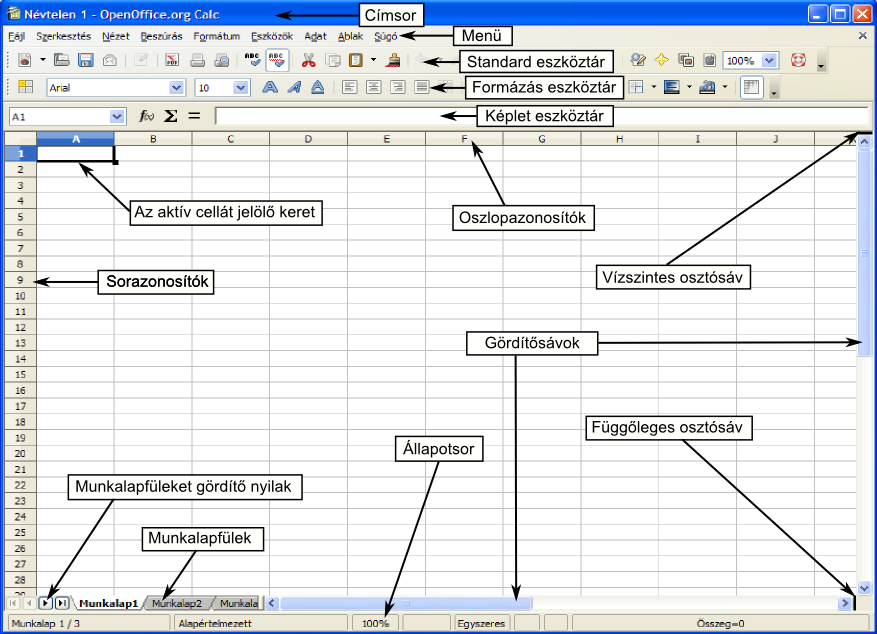
\includegraphics[width=13.999cm]{oocalcv2-img2.png}
\caption{OpenOffice.org Calc ablak}\label{Ablak}
\end{center}
\end{figure}

A \textbf{\textit{Calc}} programot elindítva figyeljük meg
ablakának részeit (\ref{Ablak} ábra). A \textbf{Címsor}ban látjuk a
 dokumentum és a program nevét. Nem mentett dokumentum esetén a
,,Névtelen'' nevet látjuk.  A
címsor alatt a \textbf{Menü} található. Ezekre a menüpontokra
kattintva kategóriákba rendezetten elérhető a program
összes funkciója. A  leggyakrabban használt parancsokat
kiadhatjuk az eszköztárak ikonjai segítségével is.
Alapértelmezés szerint három eszköztárat látunk:
\textbf{Standard}, \textbf{Formázás} és \textbf{Képlet}
eszköztár. A \textbf{Nézet} menüpont \textbf{Eszköztárak}
parancsával több eszköztár is bekapcsolható. Az
 eszköztárak pozíciója megváltoztatható az egér
,,fogd és vidd'' funkciójával, a
bal szélükön látható pontozott oszlopnál megfogva.

Az eszköztárak alatt a táblázatkezelő dokumentumablakát
láthatjuk. Egy 1024 oszlopból és 1048576 sorból álló
táblázatot, ahol az oszlopokat betűkkel (A, B, C, {\dots}, AA,
{\dots}, AMJ), míg a sorokat egész számokkal (1, 2, 3, {\dots},
1048576) jelölik. Ezt a táblázatot Munkalapnak nevezzük. A Calc
induláskor három munkalapot hoz létre automatikusan. Ezek
között a munkalapfülek segítségével válthatunk. A
munkalapfüleken a munkalapok neveit láthatjuk. A fülek
bármelyikén jobb egérgombbal kattintva, a megjelenő
gyorsmenü segítségével átnevezhetjük a munkalapokat,
illetve további munkalapokat hozhatunk létre.

A munkalapfülektől balra a lapfüleket gördítő nyilakat
találjuk. Több munkalap esetén előfordulhat, hogy nem
látjuk mindegyik munkalapfület. Ilyenkor ezekkel a nyilakkal
görgethetjük a munkalapfülek sorát.

A munkalap legkisebb elemét cellának nevezzük. Minden cellának
címe van, ami az oszlop és a sorazonosítóból tevődik
össze. Tehát a munkalap bal felső sarkában az A1-es cella
található, mellette közvetlenül a B1-es.

Az éppen használt munkalapnak mindig van aktív cellája. Ezt a
cellát keret jelöli, és a sor- és az oszlopazonosító,
amelyek metszéspontján az aktív cella található, ki van
emelve.

Az \textbf{Állapotsor} az ablak legalján található. Rajta az
aktuális munkalapra vonatkozó különböző információkat
láthatunk.

Nagyobb táblázatoknál hasznos lehet, hogy a vízszintes és a
függőleges osztósáv segítségével feloszthatjuk a
munkalapot több részre. Így megoldható, hogy egyszerre lássuk
a képernyőn a táblázat két, egymástól sok cellányi
távolságra lévő sorát vagy oszlopát.  


\section{A Súgó használata}

\begin{figure}[!h]
\begin{center}
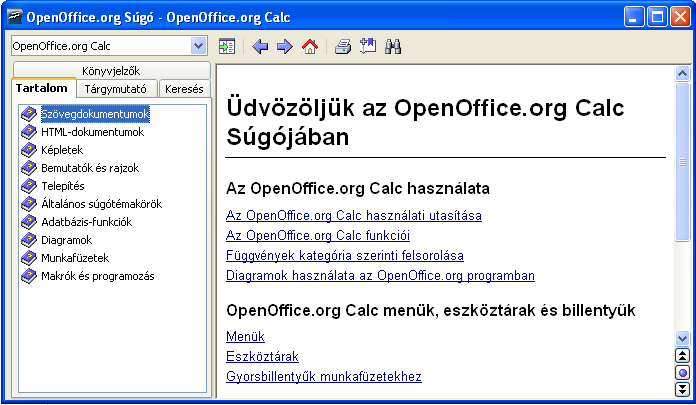
\includegraphics[width=15.999cm]{oocalcv2-img3.png}
\caption{OpenOffice.org Súgó}\label{Súgó}
\end{center}
\end{figure}

A \textit{Calc} programban igen részletes, magyar nyelvű
segítséget jeleníthetünk meg a \textbf{Súgó} menü
\textbf{OpenOffice.org Súgó} parancsával, vagy az F1
funkcióbillentyű lenyomásával. A megjelenő ablakban (\ref{Súgó}
ábra) megtaláljuk a menük, eszköztárak elemeinek
magyarázatát, a függvények kategória szerinti
felsorolását és példákat a használatukhoz, de kereshetünk
a Súgó teljes szövegében is.
A Súgó általunk hasznosnak ítélt oldalait ki is nyomtathatjuk
a \textbf{Nyomtatás\dots} paranccsal,  vagy könyvjelzőt
rendelhetünk az adott súgóoldalhoz.

A Calckal való ismerkedés során nagyon hasznos lehet, hogy a
\textbf{Súgó} menü \textbf{Mi ez?} parancsával a program
ablakának több eleméről tippet kaphatunk. Ilyenkor az egér
mutatója alakot vált, és amire mutatunk vele, arról rövid
magyarázatot olvashatunk a megjelenő szövegdobozban. \Aref{Miez}
ábrán a \textbf{Standard} eszköztár \textbf{Kivágás}
parancsáról megjelenő tippet láthatjuk.
\begin{figure}[!h]
\begin{center}
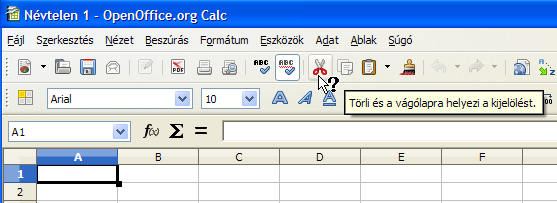
\includegraphics[width=14.736cm]{oocalcv2-img4.png}
\caption{OpenOffice.org Mi ez?}\label{Miez}
\end{center}
\end{figure}

\chapter{Első lépések a Calckal}
\thispagestyle{empty}

\section{Adatok bevitele és módosítása}

A Calc program elindítása után az A1 cella az aktív. A
billentyűzeten begépelt karakterek ebbe a cellába kerülnek. A
beírt adatot az Enterrel vagy az iránybillentyűkkel
nyugtázhatjuk. A cella tartalmát módosíthatjuk az F2
funkcióbillentyűvel, vagy kettős kattintással az adott
cellán. 

\begin{figure}[!h]
\begin{center}
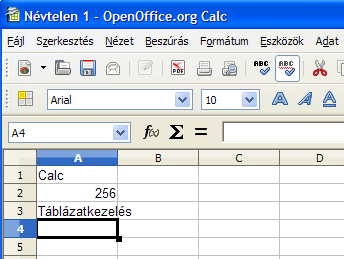
\includegraphics[width=8.102cm]{oocalcv2-img5.png}
\caption{Adatok bevitele}\label{Adatbevitel}
\end{center}
\end{figure}

\Aref{Adatbevitel} ábrán látjuk, hogy szám beírása esetén a Calc
automatikusan jobbra igazítja a tartalmat,  szöveg esetén
viszont balra. Amennyiben a beírt szöveg nem fér el a cellában,
és a tőle jobbra lévő cella üres, a cella tartalma
átcsúszik ebbe a cellába.

Adatot írva a cellába, esetünkben a B3-ba, az A3-as tartalmának
csak egy részét látjuk és a Calc erre a cella jobb szélén
megjelenő nyíllal figyelmeztet (\ref{AdatcellaTúl} ábra).

\begin{figure}[!h]
\begin{center}
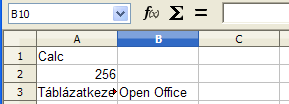
\includegraphics[width=7.645cm]{oocalcv2-img6.png}
\caption{Adatcella határán túlérő tartalom}\label{AdatcellaTúl}
\end{center}
\end{figure}

Az A oszlop szélességét módosíthatjuk, ha az
egér mutatóját az A és a B oszlopazonosító elválasztó
vonalára vezetjük és bal gombját lenyomva tartva elmozdítjuk
az egeret. Ilyenkor a leendő oszlopszélességet a Calc
megjeleníti cm-ben (\ref{Oszlopszélesség} ábra). Az oszlopazonosítók
 elválasztó vonalára kettőt kattintva a Calc automatikusan a
legtöbb karaktert tartalmazó cellához igazítja az
oszlopszélességet.

\begin{figure}[!h]
\begin{center}
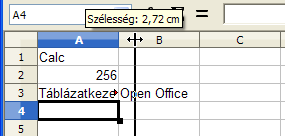
\includegraphics[width=7.539cm]{oocalcv2-img7.png}
\caption{Oszlopszélesség}\label{Oszlopszélesség}
\end{center}
\end{figure}

Számadattal nem fordulhat elő, hogy csak egy részét látjuk a
cellában. Amennyiben a számjegyek nem férnek el, a Calc mindig
kettős keresztekkel figyelmeztet erre (\ref{KeskenyOszlop}).

\begin{figure}[!h]
\begin{center}
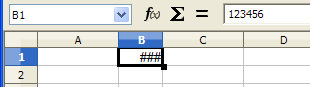
\includegraphics[width=8.2cm]{oocalcv2-img8.png}
\caption{Kicsi oszlopszélesség \#\#\#}\label{KeskenyOszlop}
\end{center}
\end{figure}

Többsoros szöveget is írhatunk a cellába, amennyiben a
Ctrl+Enter billentyűkkel zárjuk a sort. Hatására
lehetőség nyílik az új sor kezdéséhez. Ilyenkor a Calc
automatikusan megnöveli a sormagasságot.


\section{Kijelölés}

Az aktív cellán különböző formázásokat,
beállításokat végezhetünk. Több cella formátumának
 módosításához kijelöléssel meghatározhatunk cellákat,
téglalap alakú cellatartományokat. A Calcban egyszerűen
kijelölhetünk cellatartományokat: a tartomány egyik
sarokcellájára kattintva, az egér bal gombját lenyomva tartva
átlósan húzva. Egy ilyen tartományt bal felső és a jobb
alsó cellák címeivel, és közöttük kettősponttal
határozunk meg. Pl. A1:B5.

Billentyűzet segítségével, a Shift billentyűt lenyomva
tartva az iránybillentyűkkel jelölhetünk ki.

Több különálló cellát vagy cellatartományt is
kijelölhetünk. Ehhez az első kijelölése után a többit,
a Ctrl billentyűt lenyomva tartva kell kijelölnünk.

Egy oszlop vagy sor minden celláját kijelölhetjük az oszlop-,
illetve a sorazonosítóra kattintva. A munkalap bal felső
sarkában lévő üres téglalapra kattintva a munkalap minden
celláját kijelöljük (\ref{MunkalapKijelölés} ábra)

\begin{figure}[!h]
\begin{center}
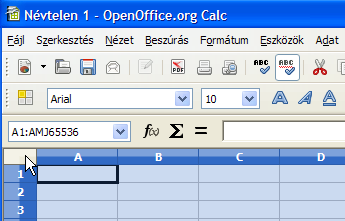
\includegraphics[width=9.126cm]{oocalcv2-img9.png}
\caption{Munkalap kijelölése}\label{MunkalapKijelölés}
\end{center}
\end{figure}

Két vagy több kijelölt cellát egyesíthetünk egy cellába a
\textbf{Formázás} eszköztár \textbf{Cellák egyesítése}
parancsával. Az így kialakult terület elfoglalja a kijelölt
cellákat, és erre a tartományra a bal cella címével
hivatkozhatunk. \Aref{CellákEgyesítése} ábrán az A3:C3 tartományt
egyesítettük egy cellává. Ennek a cellacíme A3. 

\begin{figure}[!h]
\begin{center}
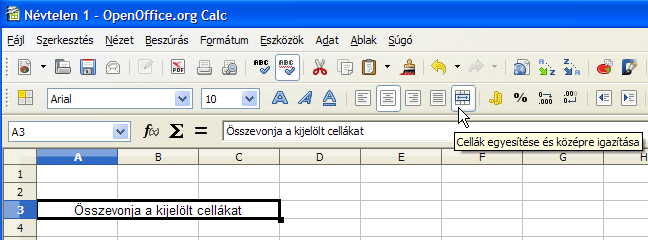
\includegraphics[width=15.999cm]{oocalcv2-img10.png}
\caption{Cellák összevonása}\label{CellákEgyesítése}
\end{center}
\end{figure}


\section{Cellák formázása}

A gyakran használt cellákra vonatkozó formátumokat
legegyszerűbben a \textbf{Formátum} eszköztáron érhetjük
el. A \textbf{Calc} képes a karakterek beírása közben
módosítani a formátumot. \Aref{CellákFormázása} ábrán látható
karakterformátumok a szöveg begépelése közben a
\textbf{Formátum} eszköztár parancsaival lettek kialakítva.

\begin{figure}[!h]
\begin{center}
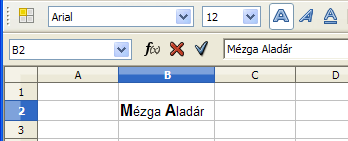
\includegraphics[width=9.206cm]{oocalcv2-img11.png}
\caption{Cellák formázása}\label{CellákFormázása}
\end{center}
\end{figure}

További, az eszköztáron nem elérhető formátumokat a
\textbf{Formátum} menü \textbf{Cellák...}, vagy a helyi menü
\textbf{Cellák formázása} paranccsal állíthatunk be. A
megjelenő párbeszédablakban a \textbf{Betűkészlet} és a
\textbf{Betűhatások} füleken a cellára vonatkozó
karakterformátumokat módosíthatjuk. 

Az \textbf{Igazítás} fülön (\ref{CellákIgazítása} ábra) beállíthatjuk az
aktuális vagy a kijelölt cellák tartalmának igazítását. A
vízszintes szövegigazítások közül az
\textbf{Alapértelmezett} a számokat jobbra, a szöveget balra
igazítja. A következő négy (balra, jobbra, középre és
sorkizárt) elérhető a Formázás eszköztáron is. A
\textbf{Kitöltött} szövegigazítás megismétli a
cellatartalmakat (számokat és szövegeket), amíg a cella
látható területét ki nem tölti.

\begin{figure}[!h]
\begin{center}
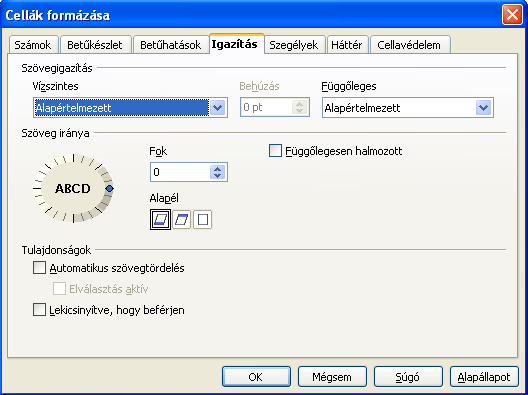
\includegraphics[width=12.97cm]{oocalcv2-img12.png}
\caption{Cellák formázása --  Igazítás}\label{CellákIgazítása}
\end{center}
\end{figure}

A \textbf{Szöveg iránya} részben megadhatjuk a kijelölt cellák
elforgatásának szögét fokokban, de megadhatjuk a
szövegirányt az ABCD feliratú körlapra kattintva is.

Figyeljük meg \aref{Cellaformátumok} ábrán látható cellaformátumokat.
A C2 cellában a vízszintes és a függőleges szövegigazítás
beállítása: \textbf{Középre.} Az \textbf{Automatikus
szövegtördelés} és az \textbf{Elválasztás} is be van
kapcsolva.

A D2 cella mind függőlegesen, mind vízszintesen középre
igazított, és a \textbf{Függőlegesen halmozott} formátum is
be van kapcsolva. 

A C1 cella balra igazított, a behúzás mértéke 10 pt.

\begin{figure}[!h]
\begin{center}
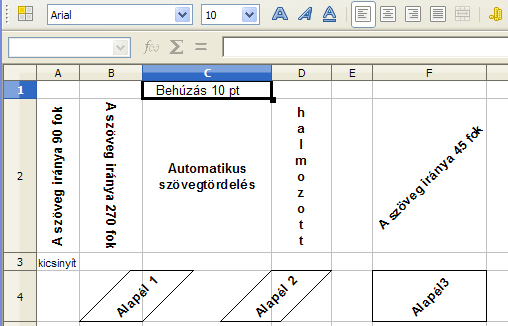
\includegraphics[width=12.439cm]{oocalcv2-img13.png}
\caption{Cellaformátumok}\label{Cellaformátumok}
\end{center}
\end{figure}

Az A3 cella betűmérete és formátuma nem különbözik a C1
celláénál, de a \textbf{Lekicsinyítve, }\textbf{hogy
beférjen} kapcsoló be van kapcsolva.

A B4, D4 és az F4 szegéllyel ellátott cellákon az Alapél
három beállítását figyelhetjük meg. Mindhárom cellában
a szöveg iránya 45 fokkal el van forgatva. A B4 cellában az
elforgatott szöveg a cella alsó szélétől kifelé jelenik
meg. A D4 esetében a felső szélétől kifelé, az F4-ben
pedig az elforgatott szöveg csak a cellába kerül.


\section{Karakterformázás}

A cella tartalmának módosításakor a kijelölt karakteren
különleges formázásokat is végrehajthatunk. Ezek
elérhetőek a \textbf{Formátum} menü \textbf{Karakter}
párbeszédablakban a  \textbf{Betűkészlet},
\textbf{Betűhatások} és \textbf{Betűhelyzet} fülekre
kattintva. Gyorsmenü segítségével szintén elérhetők
ezek a beállítások, ha a kijelölt szövegrészen az egér
jobb gombjával kattintunk (\ref{KarakterStílus} ábra).

\begin{figure}[!h]
\begin{center}
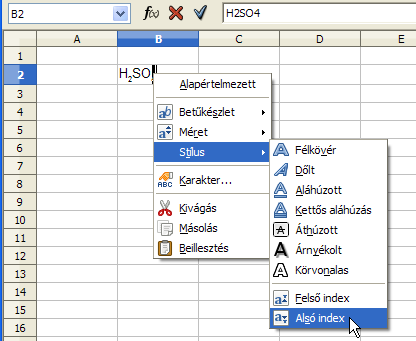
\includegraphics[width=10.005cm]{oocalcv2-img14.png}
\caption{Karakterformázás --  Stílus}\label{KarakterStílus}
\end{center}
\end{figure}

\section{Szegélyek és háttér}

A Calc alapbeállítása szerint a képernyőn látható
szürke színű rácsvonalak nyomtatásban nem jelennek meg.
Nyomtatásban is látható rácsvonalakat legegyszerűbben a
\textbf{Formátum} eszköztár \textbf{Szegélyek} ikonjára kattintva
hozhatunk létre (\ref{SzegélyekIkon} ábra).  Ilyenkor az aktív
cella, vagy a kijelölt cellatartomány az általunk választott
szegélytípust kapja.

\begin{figure}[!h]
\begin{center}
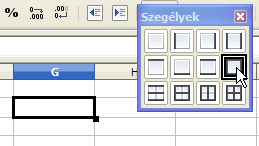
\includegraphics[width=7.351cm]{oocalcv2-img15.png}
\caption{Szegélyek ikon, menü}\label{SzegélyekIkon}
\end{center}
\end{figure}

Egyéni szegélybeállításokat a \textbf{Formátum} menü
\textbf{Cellák} parancsát választva, a párbeszédablak
\textbf{Szegélyek} lapján állíthatunk be (\ref{CellaSzegélyek} ábra).
Választhatunk vonalvastagságot, stílust, színt és akár
árnyékolást is. A \textbf{Szegély elrendezése} terület
másképp jelenik meg attól függően, hogy cellát,
cellákat egy oszlopban, cellákat egy sorban vagy nagyobb
cellatartományt jelölünk ki. Ezek a lehetőségek a
cellatartományok belső, átlós és cellákon belüli
átlós szegélyeire vonatkoznak.

\begin{figure}[!h]
\begin{center}
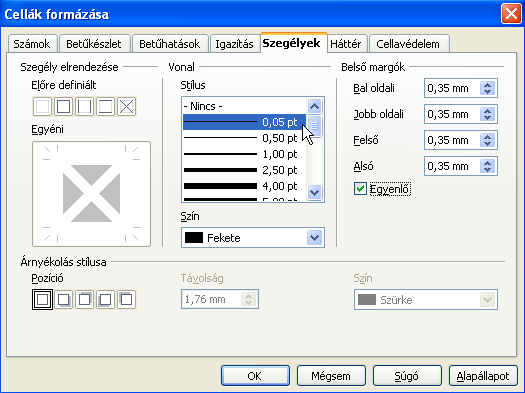
\includegraphics[width=13.891cm]{oocalcv2-img16.png}
\caption{Cellák formázása --  Szegélyek}\label{CellaSzegélyek}
\end{center}
\end{figure}

Az \textbf{Egyéni} területen kattintásokkal állíthatunk be
vonalakat. Ezek jelentése a következő:
\begin{description}
\item [Fekete vonal] -- beállítja a kijelölt cellákra a
kiválasztott stílusú vonalat. Szaggatott vonal akkor jelenik meg,
ha 0,05 pontos vonalstílus van kiválasztva.
\item [Szürke vonal] -- a kijelölt cellák megfelelő vonala
nem fog változni
\item [Fehér vonal] -- a kijelölt cellák megfelelő vonalai
törölve lesznek. 
\end{description}

Az aktív cella, vagy a kijelölt cellatartomány
háttérszínét a \textbf{Formátum} menü \textbf{Cellák}
parancsát választva, a párbeszédablak \textbf{Szegélyek}
lapján állíthatjuk be. 


\section{Munkafüzet mentése}

Munkafüzetünket a \textbf{Fájl} menü vagy a \textbf{Standard}
eszköztár \textbf{Mentés} parancsával menthetjük el. A Calc
alapértelmezett formátuma az OpenDocument, amely az irodai
dokumentumok új, nemzetközi szabványa. Az OpenDocument
munkafüzet állományának kiterjesztése .ods. A Calc képes
Microsoft Excel formátumba is menteni munkafüzetünket, amennyiben
a Fájl típusánál ezt választjuk (\ref{FájlFormátumok} ábra).

\begin{figure}[!h]
\begin{center}
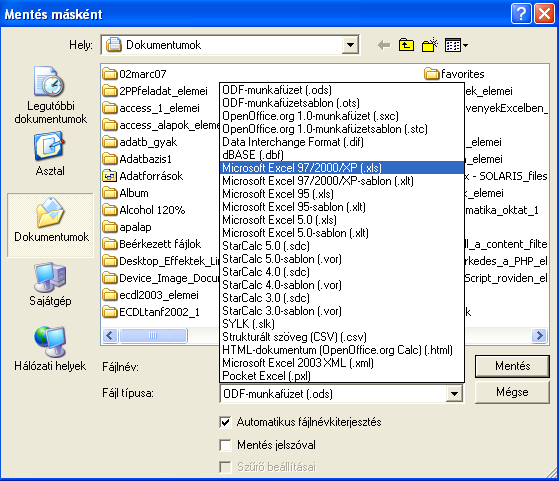
\includegraphics[width=13.79cm]{oocalcv2-img17.png}
\caption{Fájl mentése --  fájlformátumok}\label{FájlFormátumok} 
\end{center}
\end{figure}

A \textbf{Mentés} ablak, attól függően, hogy milyen
operációs rendszeren használjuk a Calcot, formailag
különbözhet. \Aref{FájlFormátumok} ábrán a Microsoft Windows XP-re
telepített Calc \textbf{Mentés} ablakát látjuk.

Az alapértelmezett mentési formátum és mentési hely
módosítható az \textbf{Eszközök} menüpont
\textbf{Beállítások} parancs kiadásakor megjelenő
párbeszédablakban (\ref{MegnyitásMentés} ábra).
A mentési helyet az \textbf{OpenOffice.org} --
\textbf{Útvonalak} --  \textbf{Dokumentumok} lehetőséget
választva módosíthatjuk. Az alapértelmezett  fájlformátum
 a \textbf{Megnyitás és mentés} -- \textbf{Általános}
ablakban állítható be, a dokumentum típusánál a
munkafüzetet választva.

\begin{figure}[!h]
\begin{center}
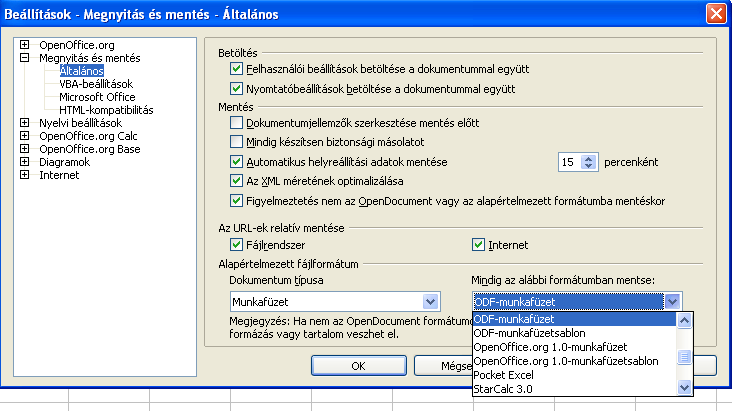
\includegraphics[width=14.999cm]{oocalcv2-img18.png}
\caption{Általános beállítások --  Megnyitás és mentés}\label{MegnyitásMentés}
\end{center}
\end{figure}


\section{1. feladat}

{\itshape
Hozzuk létre a képen látható táblázatot (\ref{1-feladat} ábra) és
mentsük el a munkafüzetet \textbf{calc01} néven OpenDocument
formátumban!}

A munkalap neve legyen ZH 01. Az egyesített B1:G1 tartományban
Ctrl+Enter segítségével hozzunk létre sortörést. A C4:G4
cellatartomány függőleges szegélyvonalai fehér
színűek.

\begin{figure}[!h]
\begin{center}
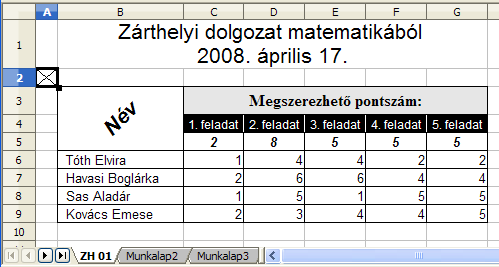
\includegraphics[width=10.673cm]{oocalcv2-img19.png}
\caption{1. feladat}\label{1-feladat}
\end{center}
\end{figure}


\chapter{Egyszerű számítások a munkalapon}
\thispagestyle{empty}

\section{Aritmetikai operátorok használata}

A Calc az egyenlő jellel (=) kezdődő matematikai
kifejezést kiszámítja és a cellában az eredményt
megjeleníti.

Az ,,=45*9+789'' beírásának 1194
lesz az eredménye. Aktívvá téve ismét a B2-es cellát a
\textbf{Képlet} eszköztár \textbf{Névdoboz}ában látjuk a
cella címét, a \textbf{Beviteli sor}ban pedig a kifejezést 
(\ref{AritmetikaiOperátorok} ábra).

\begin{figure}[!h]
\begin{center}
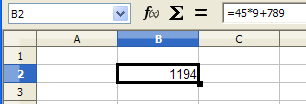
\includegraphics[width=7.094cm]{oocalcv1-img20.png}
\caption{Aritmetikai operátorok}\label{AritmetikaiOperátorok}
\end{center}
\end{figure}

A számtani alapműveletek (például összeadás, kivonás,
szorzás, osztás) végrehajtásához, számok
kombinálásához és számeredmények előállításához
az alábbi számtani műveleti jeleket használhatjuk:

\begin{description}
\item [+] (pluszjel) Összeadás;
\item [-] (mínuszjel) Kivonás; 
\item [-] (mínuszjel) Negálás; 
\item [*] (csillag) Szorzás; 
\item [/] (törtjel) Osztás;
\item [\textasciicircum] (kalap) Hatványozás (pl. 3\^{}2 --  három a négyzeten). 
\end{description}

Amennyiben egyetlen képletben több műveleti jelet vagy
operátort adunk meg, a Calc a műveleteket a következő
sorrendben hajtja végre: hatványozás, szorzás és osztás,
összeadás és kivonás. A képlet azonos prioritású
műveleteit (például szorzás és osztás) a  Calc balról
jobbra haladva értékeli ki.

A végrehajtási sorrend módosításához az elsőnek
kiértékelni kívánt képletrészt írjuk zárójelek
közé. Például az =5+2*3 eredménye 11 lesz, mivel a Calc a
szorzást az összeadás előtt hajtja végre. A képlet
összeszorozza a 2-t a 3-mal, majd hozzáad 5-öt.

Amikor a képletet módosítva zárójeleket használunk =(5+2)*3,
akkor a Calc összeadja az 5-öt és a 2-t, majd az eredményt
megszorozza 3-mal, melynek a végeredménye 21.

\section{Cellahivatkozások alkalmazása}

Legtöbbször a cellákba nem konkrét számokat, hanem
cellahivatkozásokat írunk. Módosítsuk a B2 cella tartalmát a
számok helyett az A1, B1 és C1 cellacímeket írva. Ebbe a
három cellába írjuk a kifejezés számértékeit (\ref{Cellahivatkozások}
ábra).

\begin{figure}[!h]
\begin{center}
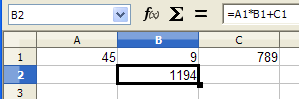
\includegraphics[width=6.909cm]{oocalcv1-img21.png}
\caption{Cellahivatkozások}\label{Cellahivatkozások}
\end{center}
\end{figure}
Módosítva az A1, B1 vagy a C1 cellák valamelyikét, a Calc
újraszámítja a cellahivatkozást tartalmazó cellát,
esetünkben a B2-t.

\section{2. feladat}
{\itshape
Készítsünk táblázatot, ami kiszámítja az A1 és a B1
cellákba írt két szám összegét, különbségét,
szorzatát és hányadosát (\ref{2-feladat} ábra)! Végezzük el az
ábrán látható formázásokat is! Ellenőrizzük az
eredményeket a következő számpárokkal: 10, 2; 81, 9 és 8,
0. Figyeljük meg a hibaüzenetet az utolsó számpár esetén a
D4 cellában. }


\begin{figure}[!h]
\begin{center}
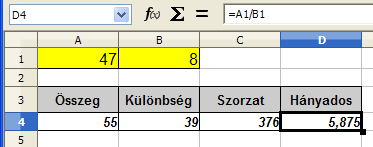
\includegraphics[width=8.867cm]{oocalcv1-img22.png}
\caption{2. feladat}\label{2-feladat}
\end{center}
\end{figure}
\section{Képletek másolása}

Táblázatos adatok esetén gyakran előfordul, hogy valamelyik
sort vagy oszlopot hasonló módon kell kiszámítani. Ilyen
esetben a képletet csak egyszer kell begépelnünk, és azt
másolással sokszorosíthatjuk.

Nevezzük át a Munkalap3 munkalapot \textbf{ZH 2}-re és
másoljuk ide az 1. feladat szegélyezett cellatartományát. Ehhez
jelöljük ki a B3:G9 tartományt, és válasszuk a
\textbf{Standard} eszköztár \textbf{Másolás} parancsát.
Ezután váltsunk a  \textbf{ZH 2} munkalap A1 cellájára és
kattintsunk a \textbf{Beillesztés} ikonra ugyanezen az
eszköztáron. Egyesítsük a G1:G3 cellákat, ebbe kerüljön
az Összesen szöveg. Végezzük el \aref{2-feladatFormázás} ábrán látható
formázásokat.

\begin{figure}[!h]
\begin{center}
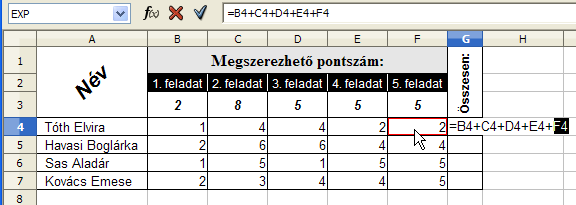
\includegraphics[width=14.238cm]{oocalcv1-img23.png}
\caption{2. feladat --  Formázás}\label{2-feladatFormázás}
\end{center}
\end{figure}

A G4 cellában számítsuk ki az első tanuló
összpontszámát. A képletben szereplő cellahivatkozásokat
egérrel is létrehozhatjuk egyszer kattintva az adott cellára. Ez
általában gyorsabb módszer, mintha a cellák címeit
gépelnénk be.

Az első tanuló összpontszámát a =B4+C4+D4+E4+F4
képlettel\footnote{Természetesen létezik a Calcban ennél
egyszerűbb megoldás is a cellatartomány összegének
kiszámítására, amit a  függvények bemutatásánál
tárgyalunk.} számítjuk ki. A második  képletet már nem
kell beírnunk, másolás segítségével létrehozhatjuk. Ehhez
vezessük az egérmutatót az aktív G4 cella jobb alsó
sarkába. Ott az keresztté változik és az egér gombját
lenyomva tartva töltsük ki (húzzuk lefelé) a G5:G7
tartományt. (\ref{2-feladatÖsszegzés} ábra)

\begin{figure}[!h]
\begin{center}
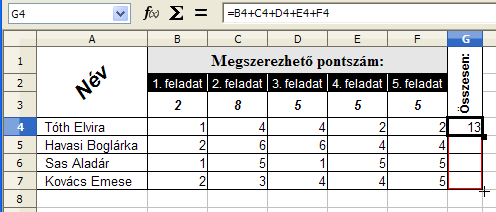
\includegraphics[width=12.122cm]{oocalcv1-img24.png}
\caption{2.  feladat --  Összegzés}\label{2-feladatÖsszegzés}
\end{center}
\end{figure}

A Calc minden cellában a megfelelő képletet hozza létre, mert
a cellahivatkozásokat tartalmazó képletet lefelé úgy
másolja, hogy növeli eggyel a cellahivatkozásokban a sorszámot.
Fölfelé másolásnál csökkenti. Az összpontszámokat úgy
is kiszámolhattuk volna, hogy először a 7. sorban lévő
képletet írjuk be, és azt másoljuk fölfelé.

Jobbra másolásnál az oszlopazonosítót ,,növeli'', ha balra másolunk,
csökkenti azt.

Amennyiben egy cella cellahivatkozásokat és számokat is tartalmaz,
akkor a képlet másolásakor az állandók nem változnak.
Például, ha egy cella tartalma =5*C1*D2+12, akkor azt lefelé
másolva   =5*C2*D3+12-t kapunk.

\clearpage
\section{3. feladat}
{\itshape
Válaszoljuk meg a következő kérdéseket, majd
ellenőrizzük a Calc segítségével:}

{\itshape
a) Az A1 cella tartalma =D3*2. Mi lesz az E5 tartalma, ha az A1 cellát
lefelé három, majd négy cellán át jobbra másoljuk?}

{\itshape
b) Az A1 cella tartalma =A8+B8-412. Mi lesz a C2 tartalma, ha az A1-et
lefelé eggyel, majd két cellán át jobbra másoljuk?}


\section{Abszolút hivatkozás}

Az eddig tárgyalt cellahivatkozásokat relatív hivatkozásoknak
nevezzük. Ez azt jelenti, hogy az ilyen hivatkozások a képletek
másolásánál automatikusan módosulnak. Vannak esetek viszont,
amikor olyan képletre van szükségünk, amelyikben egy vagy
több hivatkozás nem változik másoláskor. Ilyenkor abszolút
cellahivatkozást kell használnunk.

Abszolút hivatkozás az, ha egy az oszlop- és sorazonosító
elé egy \$ jelet írunk. Például: \$B\$3. Ez a hivatkozás
ugyanúgy a B3-as cellára mutat, de ha így szerepel a
képletekben, akkor másoláskor nem változik.

A következő feladatban áttekintjük az abszolút
cellahivatkozás használatát.

\section{4. feladat}

{\itshape
\Aref{4-feladat} ábrán egy üzletben eladott péksütemények napi adatait
látjuk. Számítsuk ki a bevételt minden napra és a heti
összbevételt is. A 8. sorban a képleteket másolással hozzuk
létre!}

\begin{figure}[!h]
\begin{center}
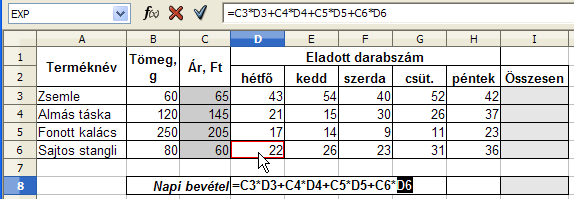
\includegraphics[width=15.185cm]{oocalcv1-img25.png}
\caption{4. feladat}\label{4-feladat}
\end{center}
\end{figure}

Szúrjunk be egy új munkalapot és nevezzük át Bevétel-re. A
hétfői bevétel kiszámítását látjuk az ábrán:
összeadjuk az egyes termékek eladásából befolyt összegeket,
amelyeket a darabszám és az ár szorzataként kapunk meg. Ezt a
képletet jobbra másolva hibás eredményt kapnánk. Ahhoz, hogy
a másolás helyes képletet hozzon létre, módosítanunk kell a
D8 tartalmát úgy, hogy az árakat megadó cellahivatkozások ne
módosuljanak. A helyes képlet tehát:
\textsf{\textbf{=\$C\$3*D3+\$C\$4*D4+\$C\$5*D5+\$C\$6*D6}}.
A \$ jeleket be is írhatjuk (AltGr+É a billentyűzeten), de
sokkal gyorsabb megoldás, ha az adott cellahivatkozásra kattintva
megnyomjuk a Shift+F4 billentyűkombinációt. A képletet jobbra
másolva így már helyes eredményt kapunk (\ref{4-feladat-2} ábra).

\begin{figure}[!h]
\begin{center}
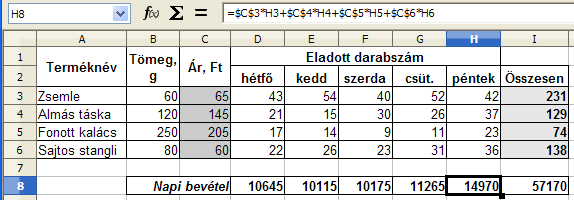
\includegraphics[width=15.185cm]{oocalcv1-img26.png}
\caption{4. feladat}\label{4-feladat-2}
\end{center}
\end{figure}


\section{Vegyes cellahivatkozások}

Relatív és abszolút cellahivatkozásokon kívül léteznek
még vegyes cellahivatkozások is. A vegyes cellahivatkozás
tartalma abszolút oszlop és relatív sor, vagy abszolút sor és
relatív oszlop. Ilyen hivatkozásokra akkor van szükség, ha azt
akarjuk, hogy a hivatkozás egyik összetevője (az oszlop- vagy
sorazonosító) állandó maradjon, a másik viszont változzon
másoláskor. Példa a vegyes hivatkozásra: =A\$1 vagy =\$A1. A
Shift+F4 billentyűkombinációt többször lenyomva
cellahivatkozás beírásakor az abszolútra, vegyesre és ismét
relatívra változik.

A vegyes hivatkozások begyakorlására készítsük el a
következő feladatot.

\section{5. feladat}
{\itshape
Hozzuk létre a természetes számok négyzeteinek táblázatát
10-től 99-ig. A képletet csak egy cellába írjuk be, a
többit másolással töltsük fel.}

\begin{figure}[!h]
\begin{center}
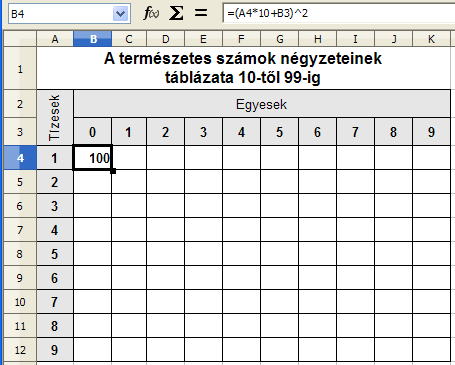
\includegraphics[width=10.037cm]{oocalcv1-img27.png}
\caption{5. feladat}\label{5-feladat}
\end{center}
\end{figure}

Új munkalapon hozzuk létre \aref{5-feladat} ábrán látható
táblázatot. Állítsuk be a cellaformátumokat. Figyeljük meg
a C4 cellába írt képletet. A képlet helyes, de jelenlegi
formájában nem másolható. Vízszintes másoláshoz úgy
kell módosítani, hogy az A4 cellacím, ami 4-es sorban tízesek
számát tartalmazza, ne változzon. Viszont ha függőlegesen
lefelé másoljuk az A4 cellacímnek A5-re kell  változnia.
Tehát az A4 cellahivatkozásban az oszlopazonosítónak
abszolútnak kell lennie, a sorazonosítónak pedig vegyesnek: \$A4.

Hasonlóképpen a B3 cellahivatkozás jobbra másoláskor
változnia kell (relatív oszlopazonosító), de lefelé
történő másoláskor nem változhat (abszolút
sorazonosító): B\$3.

Megállapíthatjuk, hogy a helyes képlet esetünkben:
\textsf{\textbf{\textcolor[rgb]{0.5019608,0.0,0.0}{=(\$A4*10+B\$3)\^{}2}}}.

Másoljuk a képletet jobbra (\ref{5-feladat-2} ábra).

\begin{figure}[!h]
\begin{center}
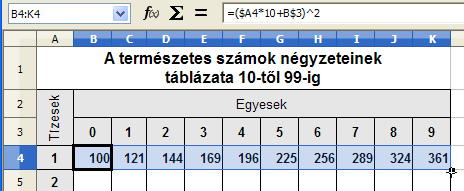
\includegraphics[width=12.275cm]{oocalcv1-img28.png}
\caption{5. feladat}\label{5-feladat-2}
\end{center}
\end{figure}

A kapott sort másoljuk lefelé, megkapva mind a 90 cellában az
eredményt (\ref{5-feladat-3} ábra).

\begin{figure}[!h]
\begin{center}
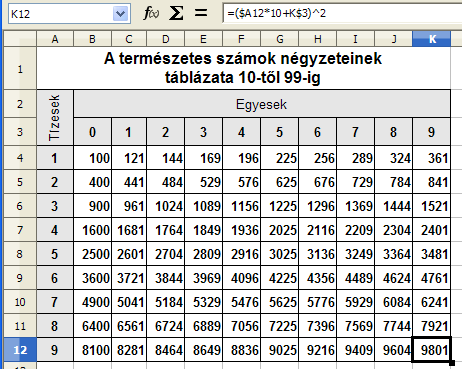
\includegraphics[width=12.222cm]{oocalcv1-img29.png}
\caption{5. feladat --  megoldás}\label{5-feladat-3}
\end{center}
\end{figure}

Térjünk vissza az előző, 4. feladatra. A D8 cellában
kiszámított hétfői bevételt jobbra másoltuk. Ilyenkor
csak a cellahivatkozás oszlopazonosító része változik.
Tehát a képletben a sorazonosítók előtti dollárjel
fölösleges. A képlet helyes eredményt ad, de --  szigorúan
véve --  itt is vegyes hivatkozást kellett volna alkalmazni. A
képlet helyesen:
\textsf{\textbf{=\$C3*D3+\$C4*D4+\$C5*D5+\$C6*D6}}.

A vegyes és az abszolút cellacímzés begyakorlására oldjuk
meg a következő feladatot.

\section{6. feladat}
{\itshape
\Aref{6-feladat} ábrán egy társasház lakásainak adatait látjuk.
Számítsuk ki a lakások havi közös költségeit, ha az a
következő összetevőkből áll:
négyzetméterenkénti alapdíj, víz és csatorna díj és
felújítási díj. A liftdíj állandó minden hónapban és
nem függ a lakás területétől. A D3 cellába írt képlet
legyen másolható minden lakásra és hónapra!}

\begin{figure}[!h]
\begin{center}
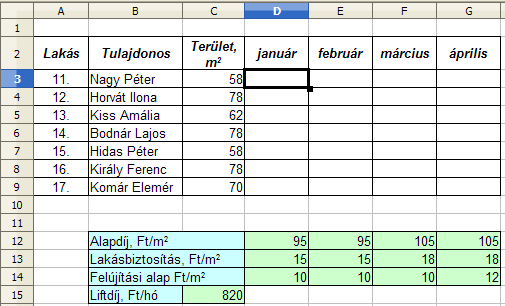
\includegraphics[width=12.813cm]{oocalcv1-img30.png}
\caption{6. feladat}\label{6-feladat}
\end{center}
\end{figure}

Az első lakás területét a C3 cella tartalmazza, a januári
költségeket pedig a D12, D13 és D14 cellák. A liftdíjat a C15
cella. A közös költséget tehát a következő képlettel
határozhatjuk meg:
\textsf{\textbf{=C3*(D12+D13+D14)+C15}}. Ahhoz, hogy
ez a képlet másolható legyen mind jobbra, mid lefelé
határozzuk meg a hivatkozások típusait. Mivel a liftdíj minden
hónapban és minden lakásra állandó,  a C15-nek abszolútnak
kell lenni. Jobbra másolásnál a születendő képleteknek
ugyanarra a lakásra  kell hivatkoznia, lefelé másolásnál
pedig a következőre. Tehát itt vegyes hivatkozást
alkalmazunk: \textsf{\textbf{\$C3}}. A díjak
esetén pedig fordítva kell eljárnunk, a vegyes hivatkozásban az
oszlopazonosítónak változni kell, a sorazonosító pedig
állandó. A végleges képlet tehát:
\textsf{\textbf{=\$C3*(D\$12+D\$13+D\$14)+\$C\$15}}. 
Figyeljük meg, hogy ez a képlet csak ilyen
hivatkozásokkal másolható a D3:G9 tartományon, bármelyik
hivatkozás módosítása hibás értékeket eredményezne.

A feladat megoldása \aref{6-feladatMegoldás} ábrán látható.

\begin{figure}[!h]
\begin{center}
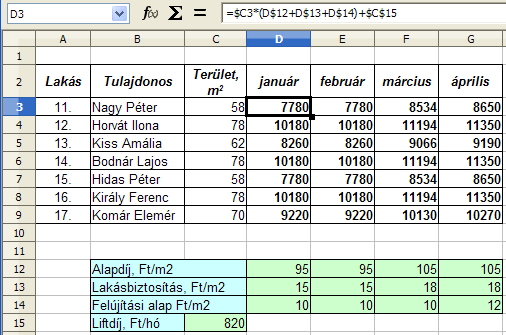
\includegraphics[width=13.386cm]{oocalcv1-img31.png}
\caption{6. feladat --  megoldás}\label{6-feladatMegoldás}
\end{center}
\end{figure}


\chapter{Függvények használata}
\thispagestyle{empty}

\section{Függvények beszúrása}

A függvények jelentősen megkönnyítik a számítási és
egyéb feladatok elvégzését a táblázatkezelő
programokban.

A függvények két részből állnak: a függvény
nevéből és argumentumból. Az argumentumot zárójelek
között kell megadnunk. Egy függvénynek több argumentuma is
lehet, ilyenkor pontosvesszővel választjuk el őket
egymástól. A függvény általános alakja tehát:
\begin{center}
=FÜGGVÉNYNÉV(argumentum1; argumentum2; ...)
\end{center}

Van olyan függvény is, amelynek nincs argumentuma, a zárójeleket
ilyenkor sem hagyhatjuk el. Például a matematikában használatos
${\pi}$ számot meg tudjuk adni cellában függvénnyel: =PI().

A leggyakrabban használt függvény a SZUM, ami összeadja az
argumentumlistájában lévő számokat. A SZUM függvény a
következő argumentummal =SZUM(A1:A4;C2) egyenértékű az
$=A1+A2+A3+A4+C2$ képlettel. Ezen az egyszerű példán is
láthatjuk, hogy a függvények használata megkönnyíti a
számításokat.

Függvényeket a \textbf{Beszúrás} menüpont
\textbf{Függvény} parancsával (Ctrl+F2) vagy a \textbf{Képlet}
eszköztár ikonjaival hozhatunk létre. Ezek közül az első
a \textbf{Függvénytündér}, a második az \textbf{Összeg}
és a harmadik a \textbf{Függvény}.

\begin{figure}[!h]
\begin{center}
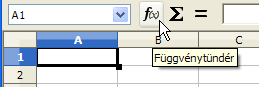
\includegraphics[width=7.751cm]{oocalcv2-img32.png}
\caption{Függvénytündér}\label{Függvénytündér}
\end{center}
\end{figure}

A \textbf{Függvény} ikon (\aref{Függvénytündér} ábrán az
,,='' feliratú) megkönnyíti a
legutóbb használt függvények ismételt kiválasztását
(\ref{FüggvényKiválasztás} ábra).
Nagyon hasznos funkció, hiszen a Calc több száz
függvénye közül egy munkalapon rendszerint csak néhányat
használunk. 

\begin{figure}[h]
\begin{center}
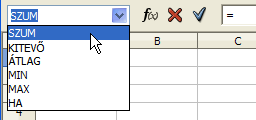
\includegraphics[width=5.772cm]{oocalcv2-img33.png}
\caption{Függvény kiválasztása}\label{FüggvényKiválasztás}
\end{center}
\end{figure}

\Aref{FüggvényKiválasztás} ábrán látható, hogy az eszköztár ikonjai is
megváltoztak: megjelent a \textbf{Mégse} és az
\textbf{Elfogadás} parancs. Ezekkel, egér segítségével is
nyugtázhatjuk a kiválasztott függvényeket és argumentumokat.

\section{Egyszerűbb statisztikai függvények használata}
(SZUM, MIN, MAX, ÁTLAG, DARAB, DARAB2, KICSI, NAGY)

A Calc program magyar nyelvű változatában általában magyar
függvénynevekkel találkozunk.\footnote{A OpenOffice.org 3.2.1-es 
verziótól kezdve} Ezek a magyar függvénynevek megegyeznek a magyar
Excelben lévőkkel. Csak azok a függvénynevek 
nincsenek lefordítva, amelyek nem léteznek a magyar Excelben, 
vagy abban nincsenek lefordítva. Ezeknek az angolul maradt 
függvényeknek a használata az angol
nyelvet nem ismerők számára sem jelenthet gondot, hiszen a
függvények magyarázata és a súgó példái magyar nyelvűek. 

A Calc súgója megkönnyíti azok dolgát, aki csak az angol függvényneveket
ismerik. A magyar megfelelő kikereséséhez válasszuk a Súgó
ablakában a \textbf{Tárgymutató}t, a \textbf{Keresett
kifejezés}hez pedig írjuk a függvény angol nevét
(\ref{SúgóÁtlag} ábra).


\begin{figure}[!h]
\begin{center}
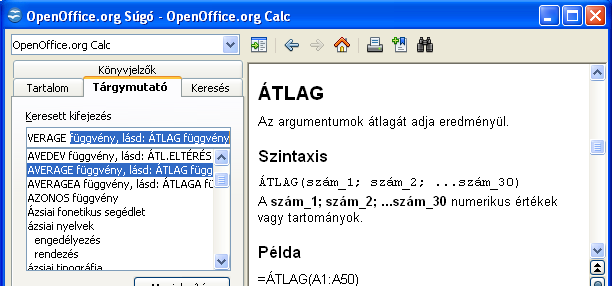
\includegraphics[width=13.193cm]{oocalcv2-img34.png}
\caption{OpenOffice.org Súgó --  Átlag}\label{SúgóÁtlag}
\end{center}
\end{figure}

\Aref{AlapvetőFüggvények} táblázatban a négy leggyakrabban használt
függvényt láthatjuk.

\begin{table}[!h]
\begin{center}
\caption{Alapvető függvények}\label{AlapvetőFüggvények}
\begin{tabular}{|m{2.5cm}|m{8cm}|m{3cm}|}
\hline
\multicolumn{1}{|c|}{\textbf{A függvény}}&
\multicolumn{1}{c|}{\textbf{Funkciója}}&
\multicolumn{1}{c|}{\textbf{A függvény}} \\
\multicolumn{1}{|c|}{\textbf{neve}} & &
\multicolumn{1}{c|}{\textbf{angol neve}} \\
\hline
SZUM & Összeadja a cellatartományban lévő számokat. & SUM \\
\hline
MIN & Az argumentumlista legkisebb értékét adja eredményül. & MIN \\
\hline
MAX & Az argumentumlista legnagyobb értékét adja eredményül. & MAX \\   
\hline
ÁTLAG & Az argumentumok átlagát adja eredményül. & AVERAGE \\
\hline
\end{tabular}
\end{center}
\end{table}

A Függvénytündér használatának begyakorlására
készítsük el a következő feladatot.


\section{7. feladat}

{\itshape
Másoljuk egy üres munkafüzetbe a \textbf{ZH 02} munkalapot. A
munkalapon töröljük a képlettel kiszámított cellák
tartalmát. Számítsuk ki az összpontszámokat a G oszlopban a
SZUM függvénnyel. A 8. sorban függvény segítségével
jelenítsük meg a feladatok és az összpontszámok átlagát.
 Határozzuk meg a legnagyobb és a legkisebb összpontszámot,
valamint azt, hogy a legtöbb  pontszámot elért tanulónak
hány pont hiányzik a maximálisan elérhetőhöz. Mentsük a
munkafüzetet \textbf{calc02} néven.}

A munkalap tartalmát átmásolhatjuk kijelölve, másolva és a
másik munkafüzetbe beillesztve azt, de gyorsabb módszer a
munkafüzet beszúrása (\textbf{Beszúrás} menüpont
\textbf{Munkalap} parancs). Itt válasszuk a \textbf{Fájlból}
kapcsolót, majd a \textbf{Tallózás} parancs segítségével
adjuk meg annak a munkafüzetnek a  nevét, amelyik a szükséges
munkalapot tartalmazza (\ref{7-feladatMunkalap} ábra).

\begin{figure}[!h]
\begin{center}
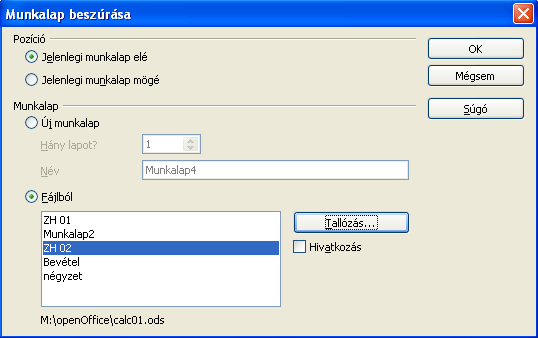
\includegraphics[width=11.235cm]{oocalcv2-img35.png}
\caption{7. feladat --  Munkafüzet beszúrása}\label{7-feladatMunkalap}
\end{center}
\end{figure}

Jelöljük ki a ZH 02 munkalap nevét és szúrjuk be az aktuális
munkafüzetünkbe.
A munkalapon jelöljük ki a G4:G7 tartományt és a
,,Backspace'' billentyűvel
töröljük a tartalmát. 

\begin{figure}[!h]
\begin{center}
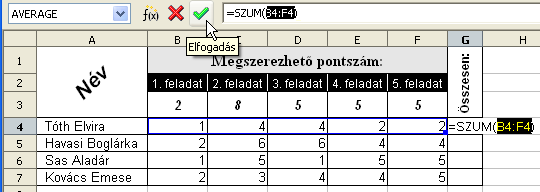
\includegraphics[width=11.288cm]{oocalcv2-img36.png}
\caption{7. feladat}\label{7-feladat}
\end{center}
\end{figure}

Tegyük aktívvá a G4 cellát és kattintsunk a \textbf{Képlet}
eszköztár \textbf{Összeg} ikonjára. A cellában megjelenik a
SZUM függvény és a megfelelő argumentumok is. A Calc az
aktív cellától balra egy számsort talált és azt beírta a
SZUM függvénybe argumentumként. Ez nagyon hasznos funkció,
hiszen gyakran fordul elő, hogy egy sor végén, vagy egy oszlop
alján kell annak összegét kiszámolni. A kék színű keret
 mutatja az automatikusan meghatározott tartományt (\ref{7-feladat} ábra).

A képletet három cellán át lefelé másolva megkapjuk mind a
négy tanuló összpontszámát.

Az A8 cellába írjuk az ,,Átlag''
szót és a B8 cellában válasszuk a függvénytündért 
(\ref{7-feladatFüggvény} ábra).

\begin{figure}[!h]
\begin{center}
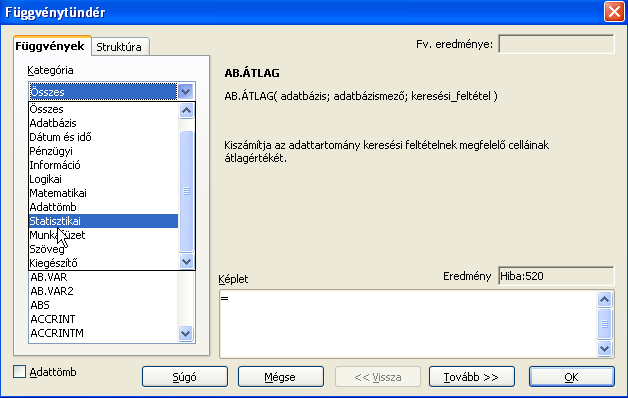
\includegraphics[width=13.999cm]{oocalcv2-img37.png}
\caption{7. feladat --  függvénytündér}\label{7-feladatFüggvény}
\end{center}
\end{figure}

\begin{figure}[!h]
\begin{center}
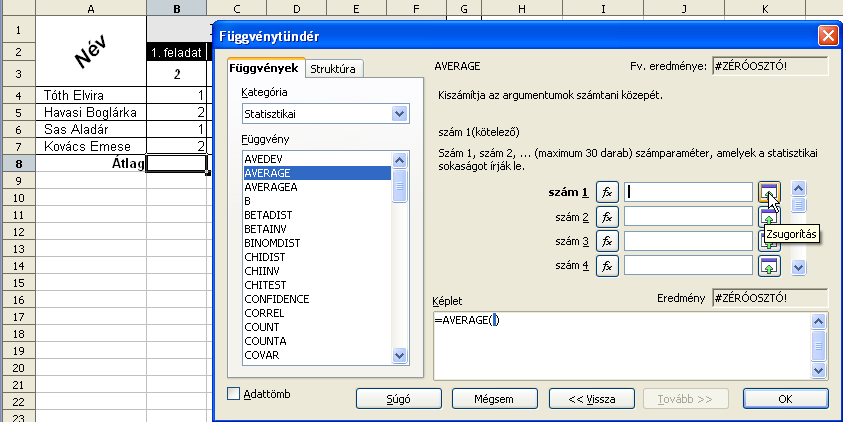
\includegraphics[width=15.999cm]{oocalcv2-img38.png}
\caption{7. feladat }\label{7-feladatArgumentum}
\end{center}
\end{figure}

Az ablakban kategóriákba rendezetten találjuk a Calc összes
függvényét. Egy függvényt kiválasztva az ablak jobb
oldalán annak a magyarázatát olvashatjuk. A \textbf{Statisztikai}
kategóriából válasszuk az ÁTLAG függvényt. A
\textbf{Tovább} gombra kattintva a párbeszédablak jobb oldalán
megjelennek az argumentumbeviteli mezők (\ref{7-feladatArgumentum} ábra).
Jelöljük ki a B4:B7 tartományt és a cellahivatkozás megjelenik az első
beviteli mezőben. Természetesen megadhatunk szám- és egyéb
értékeket, illetve hivatkozásokat a párbeszédablak megfelelő részeiben.  

A \textbf{Zsugorítás} ikon lecsökkenti a párbeszédablakot a
beviteli mező méretére. Így könnyebb a szükséges
hivatkozást megjelölni a lapon. Az ikon ezután automatikusan
átalakul a \textbf{Maximalizálás} ikonra. Erre kattintva a
párbeszédablakot visszaállíthatjuk eredeti méretére.

Bonyolultabb függvények esetén hasznos lehet a \textbf{Súgó}
parancs. A megjelenő ablakban részletes leírást és
példákat olvashatunk a kiválasztott függvényről.

Másoljuk a függvénytündérrel létrehozott B8 cellát jobbra
minden feladat és a csoport összpontszám átlagának
kiszámításához.

A legtöbb és a legkevesebb összpontszámot jelenítsük meg a
B11 és B10 cellákban a MAX és MIN függvények
segítségével. A B12 cella azt a pontszámot mutatja, amennyivel
kevesebbet ért el a legjobb tanuló az elérhető maximumnál.
Ennek kiszámításához is használhatjuk a
függvénytündért az első függvény megadása után, a
 mínusz jelet beírva a Képlet párbeszédablakba és megadva
a második függvényt (\ref{7-feladatMásodik} ábra).

\begin{figure}[!h]
\begin{center}
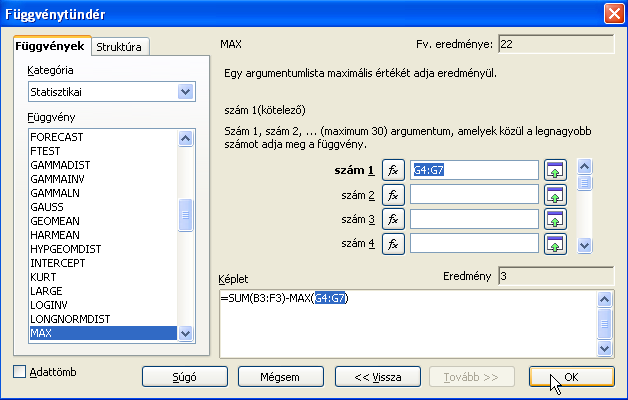
\includegraphics[width=15.999cm]{oocalcv2-img39.png}
\caption{ 7. feladat}\label{7-feladatMásodik}
\end{center}
\end{figure}

Amennyiben pontosan ismerjük a használni kívánt függvény
szintaxisát, nem kell feltétlenül használnunk a
függvénytündért, a cellába közvetlenül is beírhatjuk a
kifejezést.

\clearpage
Az elkészült feladat \aref{7-feladatMegoldás} ábrán látható.

A következő feladatban \aref{StatisztikaiFüggvények} táblázatban
felsorolt statisztikai függvényeket fogjuk használni.

\begin{figure}[!h]
\begin{center}
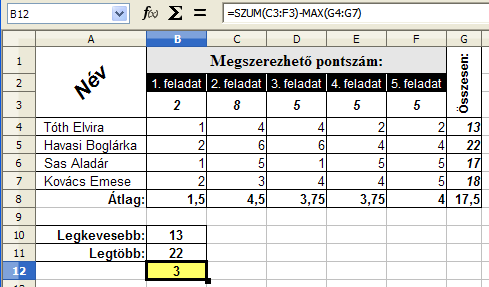
\includegraphics[width=14.936cm]{oocalcv2-img40.png}
\caption{7. feladat}\label{7-feladatMegoldás}
\end{center}
\end{figure}

\begin{table}[!h]
\begin{center}
\caption{Statisztikai függvények}\label{StatisztikaiFüggvények}
\begin{tabular}{|m{2.5cm}|m{8cm}|m{3cm}|}
\hline
\multicolumn{1}{|c|}{\textbf{A függvény}}&
\multicolumn{1}{c|}{\textbf{Funkciója}}&
\multicolumn{1}{c|}{\textbf{A függvény}} \\
\multicolumn{1}{|c|}{\textbf{neve}} & &
\multicolumn{1}{c|}{\textbf{angol neve}} \\
\hline
DARAB &
Megszámolja, hány szám van a paraméterlistában. A szöveges
bejegyzéseket kihagyja. &
COUNT\\ \hline
DARAB2 &
Megszámolja, hány érték van a paraméterlistában. A
szöveges elemek is számítanak. &
COUNTA\\ \hline
KICSI &
Kiszámítja egy adathalmaz $k$-adik legkisebb értékét. &
SMALL\\ \hline
NAGY &
Kiszámítja egy adathalmaz $k$-adik legnagyobb értékét. &
LARGE\\ \hline
\end{tabular}
\end{center}
\end{table}

\section{8. feladat}

{\itshape
\Aref{8-feladat} ábrán egy iskolai futóverseny eredményeit látjuk. Hozzuk
létre a calc02 munkafüzet második munkalapján az alábbi
táblázatot. A D oszlopban jelenjen meg a tanulók jobbik
eredménye. A G oszlop számadatait függvény segítségével
számítsuk ki.}

\begin{figure}[!h]
\begin{center}
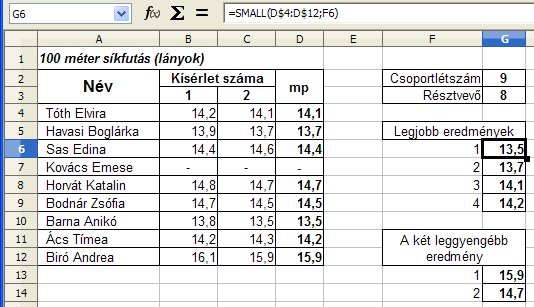
\includegraphics[width=14.125cm]{oocalcv2-img41.png}
\caption{8. feladat}\label{8-feladat}
\end{center}
\end{figure}

A csoportlétszámot a DARAB2 függvénnyel, a résztvevők
számát pedig a DARAB-bal számíthatjuk ki. Az argumentumlista
lehet ugyanaz (D4:D12), hiszen a DARAB csak a számokat tartalmazó
cellák darabszámát adja meg.

A KICSI függvénnyel meghatározhatjuk egy cellatartomány $k$-adik
legkisebb értékét. Két kötelező paramétere van: az
elsővel a tartományt adjuk meg, a másodikkal meghatározzuk,
hogy hányadik legkisebb elemre van szükségünk. Figyeljük meg
\aref{8-feladat} ábrán, hogy ez a paraméter relatív cellahivatkozás
(F6). A képlet másolásakor ez az argumentum a megfelelő
értéket fogja felvenni. Az első paraméternél viszont vegyes
cellahivatkozást használunk, hogy minden másolt függvény
ugyanarra  a tartományra hivatkozzon.

A G13:G14 tartományt hasonlóan számítjuk ki, csak itt a NAGY
függvényt alkalmazva.


\chapter{Számformátumok}
\thispagestyle{empty}

\section{Százalék és pénznem formátum}

A számokat tartalmazó cellákon speciális formázásokat
állíthatunk be. A leggyakrabban használt számformátumok az
eszköztáron is elérhetők: százalék és a pénznem
formátum. E két alapvető formátum megértéséhez írjuk
be a következő adatokat (\ref{Számformátumok} ábra).

\begin{figure}[!h]
\begin{center}
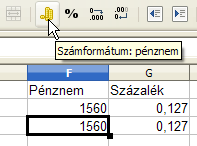
\includegraphics[width=5.211cm]{oocalcv1-img42.png}
\caption{Számformátumok}\label{Számformátumok}
\end{center}
\end{figure}

Az F3 cellán állítsunk be pénznem-, a G3 cellán pedig
százalékformátumot. Látjuk \aref{SzázalékFormátum} ábrán, hogy a pénznem
formátum ezres csoportosítást, két tizedesjegynyi pontosságot
állított be és hozzáadta az alapértelmezett pénznem
megjelölést. A százalék formátum a számot százzal
megszorozva, két tizedesjegynyi pontossággal és a
százalékjellel kiegészítve mutatja.

\begin{figure}[!h]
\begin{center}
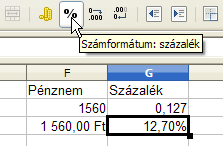
\includegraphics[width=5.898cm]{oocalcv1-img43.png}
\caption{Százalék formátum}\label{SzázalékFormátum}
\end{center}
\end{figure}

A tizedesjegyek számát növelhetjük és csökkenthetjük a
\textbf{Formátum} eszköztár \textbf{Számformátum: tizedesjegy
hozzáadása} és a \textbf{Számformátum: Tizedesjegy
törlése} kapcsolókkal. A Calc a matematika szabályai szerint
kerekít a tizedesjegyek számának csökkentésekor, de vegyük
figyelembe, hogy ilyenkor a cellában kerekítve látjuk a
számértéket, de a cella tartalma közben nem változik.
Esetünkben, ha nullára csökkentjük a tizedesjegyek számát a
G3 cellában, abban 13\%-ot fogunk látni, de a cella tartalma
továbbra is 0,127 marad.

A százalékformátum ilyen megvalósítása megkönnyíti a
százalékszámításokat: pl. az A1 cellába írt szám B1
cellába felvett százalékát a két cella szorzatával
számíthatjuk ki.

A \textbf{Formátum} eszköztár \textbf{Számformátum:
Általános} kapcsolóval törölhetjük a számformátumokat a
kijelölt cellákon, és a cella ismét alapértelmezett
számformátumú lesz.


\section{9. feladat}
{\itshape
Egy üzlet 20 db péksütemény vásárlásakor 5\%, 50 db
esetén 8\% kedvezményt ad. Számítsuk ki a kedvezményes
árakat a D2:D6 és az E2:E6 tartományokban a D10, D11 cellákban
felvett százalékértékekkel számolva (\ref{9-feladat} ábra).}

{\itshape
Az F oszlopban számítsuk ki egy kilogramm péksütemény árát
az eredeti áron számolva. Ezekből az árakból határozzuk
meg, hogy hány százalékkal drágább a fonott kalács mint a
zsemle.}

{\itshape
A táblázatot a calc02 munkafüzet harmadik munkalapján hozzuk
létre, amelyiket nevezzünk át Kedvezmény-re.}

\begin{figure}[!h]
\begin{center}
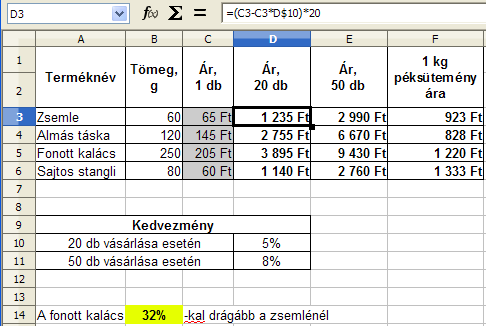
\includegraphics[width=12.857cm]{oocalcv1-img44.png}
\caption{9. feladat}\label{9-feladat}
\end{center}
\end{figure}

\Aref{9-feladat} ábrán figyeljük meg a D3 cella tartalmát:
\textsf{\textbf{=(C3-C3*D\$10)*20}}. Az eredeti árból (C3) kivonjuk
a kedvezményt, amit az eredeti ár és a kedvezmény szorzatával
(C3*D\$10) határozunk meg. Ne feledjük, hogy a D10 cella
számértéke 0,05.

A képletben zárójelből kiemelve a C3-at a következő
kifejezést kapjuk  \textsf{\textbf{=20*C3*(1-D\$10)}}.

Az E3 cellát ezzel a módszerrel számítsuk ki (\ref{9-feladatE3} ábra).

\begin{figure}[!h]
\begin{center}
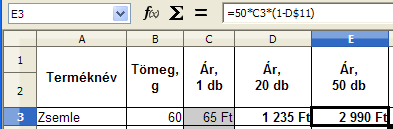
\includegraphics[width=10.396cm]{oocalcv1-img45.png}
\caption{9. feladat}\label{9-feladatE3}
\end{center}
\end{figure}

Az F oszlopban egy kilogramm péksütemény árát a
\textsf{\textbf{=}}\textsf{\textbf{B3/C3*1000}} képlettel
számíthatjuk ki, hiszen a B3/C3 egy gramm árát adja meg.

Azt, hogy hány százalékkal több az F5 mint az F3, egy tört
adja meg, aminek számlálója a két cella különbsége,
nevezője pedig az F3. A B14 cella tartalma tehát:
\textsf{\textbf{=(F5-F3)/F3}}, számformátuma százalék,
tizedeshelyek száma nulla.


\section{Dátum- és időformátum}

A Calc a dátumot egész számként tárolja, mégpedig egy
dátumértékhez viszonyított sorszámként. Alapértelmezés
szerint a kezdődátum 1899. december 30., ez a dátum a
nullának felel meg. Az ezt követő az egyes számnak, és
így tovább. A kezdődátumnál korábbi dátumokat a program
nem értelmezi.

\begin{figure}[!h]
\begin{center}
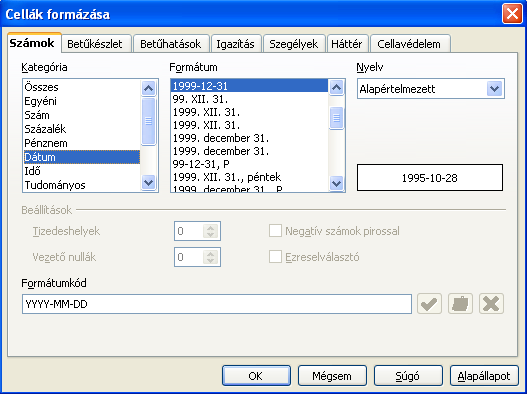
\includegraphics[width=13.944cm]{oocalcv1-img46.png}
\caption{Dátumformátumok}\label{Dátumformátumok}
\end{center}
\end{figure}

Minden számformátumot, így a dátumformátumot is
módosíthatjuk a \textbf{Formátum} menü \textbf{Cellák}
ablakában a \textbf{Számok} fület választva. \Aref{Dátumformátumok} ábrán
az A1 cella számformátumát látjuk, aminek tartalma 35000. A
\textbf{Dátum} kategóriát választva az
előnézetmezőben láthatjuk, hogy ennek a  számnak az
1995-10-28 dátum felel meg alapértelmezett dátumformátum
esetén. A \textbf{Formátumkód} ebben az esetben YYYY-MM-DD.

A Formátumkódot szerkeszthetjük is, a fenti példából is
látjuk, hogy négy Y betű az évszámot jeleníti meg. A
dátumformátum gyakran használt formátumkódjait \aref{DátumFormátumkódjai}
ábrán láthatjuk.

\begin{figure}[!h]
\begin{center}
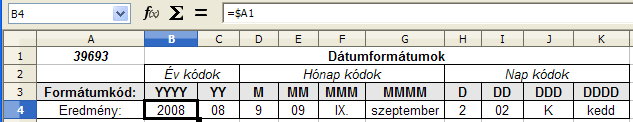
\includegraphics[width=15.999cm]{oocalcv1-img47.png}
\caption{Dátumformátumok formátumkódjai}\label{DátumFormátumkódjai}
\end{center}
\end{figure}

A B4 cella tartalma =\$A1, és ezt másoljuk a K4 celláig. Tehát a
B4:K4 tartomány minden cellája az A1 tartalmát mutatja. Ezeken a
cellákon a fölöttük látható dátumformátum van
beállítva.

Egyéni dátumformátumok használatára látunk három
példát \aref{EgyediDátumformátumok} ábrán.

\begin{figure}[!h]
\begin{center}
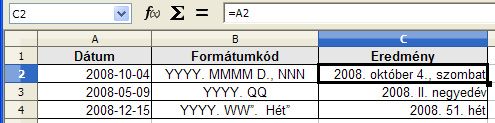
\includegraphics[width=13.095cm]{oocalcv1-img48.png}
\caption{Egyedi dátumformátumok}\label{EgyediDátumformátumok}
\end{center}
\end{figure}

A formátumkódot kiegészíthetjük tetszőleges szöveggel
is, ilyenkor a szöveget aposztrófjelek
(''...'') közé kell zárni.

Mind a dátumformátumot, mind a százalék- és
pénznemformátumot a Calc beíráskor automatikusan alkalmazza.
Ilyenkor a cella --  mint számok beírásakor --  jobbra igazított
lesz. Írjuk három cellába a következő tartalmakat: 2000Ft,
15\%, 2008.08.01. Figyeljük meg, hogy a Calc automatikusan alkalmazza
a pénznem, százalék és a dátum formátumokat. A cellák
tartalma pedig 2000, 0,15 és 39661 lesz, amit ellenőrizhetünk a
\textbf{Formátum} eszköztár \textbf{Számformátum:
Általános} parancsát alkalmazva.

A Calcban időértéket a szám tizedesjel utáni része
határozza meg.

Írjuk a 39700,5 számot egy cellába és válasszuk \aref{Időformátumok}
ábrán látható dátumformátumot. Látjuk,  hogy
esetünkben a 0,5 szám tizenkét óra nulla perc nulla
másodpercnek felel meg.

\begin{figure}[!h]
\begin{center}
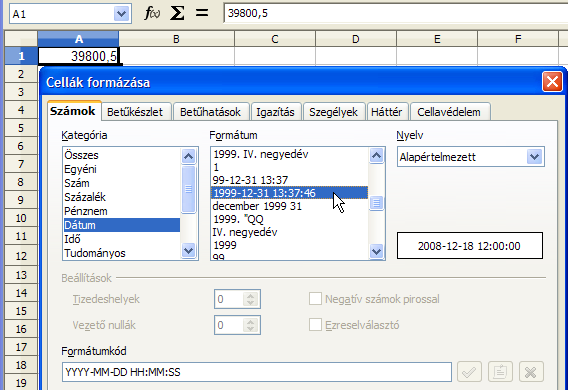
\includegraphics[width=15.027cm]{oocalcv1-img49.png}
\caption{Időformátumok}\label{Időformátumok}
\end{center}
\end{figure}
Megadhatunk dátum nélküli időértéket is,
értelemszerűen ilyenkor a szám egész része nulla lesz.

\Aref{Időformátumok} ábrán látjuk, hogy az előnézetmezőben látható
időformátumnak (12:00:00) a HH:MM:SS formátumkód felel meg.
További dátum- és időformátumokat \aref{TovábbiIdőformátumok} ábrán
találunk.

\begin{figure}[!h]
\begin{center}
\includegraphics[width=13.995cm]{oocalcv1-img50.png}
\caption{További időformátumok}\label{TovábbiIdőformátumok}
\end{center}
\end{figure}

\clearpage
\section{Számformátumkódok}

Egyedi számformátumkódok használatával meghatározhatjuk,
hogy milyen formában jelenjenek meg a beírt számok a cellákban.
Legfeljebb három, egymástól pontosvesszővel elválasztott
formátumkódot határozhatunk meg egy cellára. Az első rész
a pozitív értékekre, a második a negatívokra és a harmadik
a nullára fog vonatkozni. Akár feltételeket is megadhatunk a
három részhez, a formátumkódok csak a feltételek
teljesülésekor hatnak.

Számok jelölésére a nullát (0) vagy a kettős keresztet
(\#) használhatjuk helykitöltőként
számformátumkódokban. A \# csak a lényeges számjegyeket
jeleníti meg, míg a 0, nullákat jelenít meg, ha a kód több
jegyből áll mint a beírt szám. Néhány
számformátumkódot egyszerűen beállíthatunk a
\textbf{Szám} kategóriában (\ref{SzámFormátumkódok} ábra).

\begin{figure}[!h]
\begin{center}
\includegraphics[width=15.027cm]{oocalcv1-img51.png}
\caption{Szám formátumkódok}\label{SzámFormátumkódok}
\end{center}
\end{figure}

Léptetőnyilak segítségével módosíthatjuk a tizedeshelyek
és a vezető nullák számát. Az \textbf{Ezreselválasztó}
bekapcsolása a \#\#\# kódrészletet hozza létre, ami ezres
csoportokba rendezi a szám egész részét. A \textbf{Negatív
számok pirossal} kapcsoló a pontosvessző, színkód [RED]
és a mínusz jel után megismétli a számformátumot. Negatív
számot írva a cellába az piros színű lesz, ezres
csoportosítású, két tizedes számjegyre kerekítve.
Kettőnél kevesebb tizedes számjegy esetén, azokat nullával
helyettesíti.

Kérdőjel (?) felhasználásával létrehozhatunk
formátumkódot, ami tört alakban jeleníti meg a számot a
cellában. A \#?/? formátumkód és 2,5 cellatartalom esetén a
cellában a következő kifejezést fogjuk látni: 2~$1/2$.

A tudományos számformátum segítségével nagyon nagy, vagy
nagyon kicsi számok tömör megjelenítését valósíthatjuk
meg. 200000000 (kétszázmillió) leírható
2*10\textsuperscript{8} módon is, amit a Calc a
következőképpen jelenít meg: 2,00E+8. A formátumkód ebben
az esetben: 0,00E+\#.

A következő formátumkód négy részből áll, a negyedik
akkor fog végrehajtódni, ha a cellába nem számot írunk. Ez
hasznos lehet, hiszen figyelmezteti a felhasználót, ha az
például a 0 számjegy helyett O betűt ír:\\
{\sffamily\bfseries
[MAGENTA]\#\#\#0"db";[RED]-\#\#\#0"db";[GREEN]\#\#\#0"db";"Ön nem számot írt!"}.

Tehát a formátumkód, pozitív számot beírva, azt ezres
csoportosítással egészre kerekítve, magenta színnel
jeleníti meg, a szám után szóköz és
''db'' karakterekkel. Negatív
szám és nulla beírása esetén a kódban megadott színnel
jelennek meg a számok, a többi formátum ugyanaz mint pozitív
számnál. Szöveg beírásakor (pl. 5OO) a következő
figyelmeztető üzenet jelenik meg: ,,Ön nem
számot írt!'' Érdekes, hogy a kerekítés
miatt az is előfordulhat, hogy három különböző
színű ,,0 db''-t látunk a
cellában. Ilyen számok pl. a -0,2; 0 és 0,2. Mindhárom szám
egészre kerekítve a cellában ,,0~db''-ként jelenik meg,
de a színük magenta, piros és zöld.

A Calcban a következő színkódokat használhatjuk: CYAN
(cián), BLACK (fekete), MAGENTA (magenta), WHITE (fehér), GREEN
(zöld), BLUE (kék), RED (piros) és YELLOW (sárga).

Meghatározhatunk olyan számformátumot, ami csak bizonyos
feltétel esetén teljesül. A feltételekben számokat és
matematikai operátorokat használhatunk. A Calc súgójában a
következő példát találjuk a feltételes
számformátumra:


{\sffamily\bfseries
[BLUE][<0]\#,0"${}^\circ$C";[RED][>=30]\#,0"${}^\circ$C";[BLACK]\#,0"${}^\circ$C"}.

Ezt a formátumot alkalmazva egy cellára, a beírt negatív szám
kék színű lesz, 0 és 30 fok között fekete, 30 és
annál nagyobb pedig piros. Mindhárom esetben a számok után
megjelenik a ,,$^\circ$C'' kifejezés.


\chapter{Diagramok}
\thispagestyle{empty}

Diagramok segítségével grafikusan ábrázolhatjuk a
táblázatok számadatait. A diagramok automatikusan követik a
táblázat változásait. A Calc az adatok módosítását
követően újraépíti a diagramot. Többféle diagramtípus
közül választhatunk és az elkészült diagramokat utólag is
módosíthatjuk.


\section{Diagramtündér használata}

A \textbf{Beszúrás} menü vagy a \textbf{Standard} eszköztár
\textbf{Diagram} parancsával kezdhetünk hozzá a diagram
elkészítéséhez. Mindkét esetben a \textbf{Diagramtündér}
ablaka jelenik meg, ami végigvezet minket a diagram
elkészítésének négy lépésén. Megkönnyíti a diagram
létrehozását, ha a Diagramtündér indítása előtt
kijelöljük azt a tartományt vagy tartományokat, amelyekből
diagramunk felépül.

Nyissuk meg a calc01 munkafüzetet és a 4. feladat adatai alapján
készítsünk diagramot, ami a napi eladásokat mutatja.
Jelöljük ki az A3:A6, majd a Ctrl billentyűt lenyomva tartva a
D3:H6 tartományt (\ref{DiagramTartomány} ábra).

\begin{figure}[!h]
\begin{center}
\includegraphics[width=15.159cm]{oocalcv1-img52.png}
\caption{Diagram készítése -- tartomány kijelölése}\label{DiagramTartomány}
\end{center}
\end{figure}

Indítsuk el a Diagramtündért. Az első lépésben
kiválaszthatjuk a diagram típusát és azon belül az
altípust. A számadatok típusa általában meghatározza a
választható kategóriákat. Válasszuk az \textbf{Oszlop}
diagramtípust és a \textbf{Halmozott} altípust (\ref{DiagramTípus} ábra).

\begin{figure}[!h]
\begin{center}
\includegraphics[width=15.999cm]{oocalcv1-img53.png}
\caption{Diagram készítése --  diagramtípusok}\label{DiagramTípus}
\end{center}
\end{figure}

A diagramtündér használata közben a munkalapon kék színnel
vannak kiemelve a kiindulási cellák, és láthatjuk az e cellák
adatai alapján létrejött, általunk választott típusú
diagramot is. Figyeljük meg, hogyan változik a diagram a normál
és a halmozott altípust választva. 

A Shift+F1 billentyűkombináció segítségével, a
Diagramtündér ablakának elemeiről részletes magyarázatot
olvashatunk, ha az egér mutatóját az adott elemre vezetjük.

A Tovább gombra kattintva a függvénytündér második
lépése, az \textbf{Adattartomány} következik (\ref{DiagramAdat} ábra).
 Itt kijelölhetjük, vagy módosíthatjuk a diagram forrását.

\begin{figure}[!h]
\begin{center}
\includegraphics[width=15.999cm]{oocalcv1-img54.png}
\caption{Diagram készítése --  adattartomány}\label{DiagramAdat}
\end{center}
\end{figure}

Esetünkben az adattartomány két, pontosvesszővel
elválasztott, abszolút címzésű cellatartomány, ahol a
cellacímek előtt a munkalap nevét látjuk. Tehát a
\textbf{\$Bevétel.\$A\$3:\$A\$6} hivatkozás a Bevétel nevű
munkalap A3:A6 tartományát jelöli abszolút címzéssel. Így
hivatkozhatunk munkalapok között cellatartományokra a Calckal.

Amennyiben szükséges, hozzáadhatunk adattartományt
pontosvesszőt írva a meglévők után és az
\textbf{Adattartomány kijelölése} gombra kattintva (\aref{DiagramAdat}
ábrán az egér rá mutat). A Ctrl billentyűt lenyomva tartva
egérrel adhatunk meg további tartományokat. 

Ebben a feladatban attól függően, hogy az \textbf{Adatsorok
sorokban} vagy az \textbf{Adatsorok oszlopokban} választókapcsoló
közül melyik aktív, a diagram vízszintes tengelyére a
péksütemények nevei vagy a hét napjai kerülnek. Válasszuk
az \textbf{Adatsorok sorokban} kapcsolót.

\textbf{Az első sor legyen címke} és \textbf{Az
első}\textbf{ oszlop legyen címke} kapcsolók
automatikusan aktívak mert  a kijelölt területen az első sor
és az első oszlop cellái szöveges információt
tartalmaznak.

A következő lépés az \textbf{Adatsorok} (\ref{DiagramAdatsor} ábra).
Ebben az ablakban az adatsorok sorrendjét módosíthatjuk, és ha
szükséges, újabb adatsorokat adhatunk a diagramhoz.

\begin{figure}[!h]
\begin{center}
\includegraphics[width=15.499cm]{oocalcv1-img55.png}
\caption{Diagram készítése --  adatsorok}\label{DiagramAdatsor}
\end{center}
\end{figure}

Az adatsorok valamelyikét választva látjuk, hogy melyik
cellatartomány tartalmazza az adott adatsor számértékeit és
melyik cellában van az adatsor neve.

A \textbf{Kategóriák} részben látható cellatartomány a
diagramon az x tengely felirata lesz. Esetünkben a hét napjai
kerüljenek Ehhez válasszuk az \textbf{Adattartomány
kijelölése} kapcsolót és jelöljük ki a D2:H2 tartományt.

\begin{figure}[!h]
\begin{center}
\includegraphics[width=15.499cm]{oocalcv1-img56.png}
\caption{Diagram készítése --  diagramelemek}\label{DiagramElemek}
\end{center}
\end{figure}

A diagramtündér utolsó, negyedik ablakában címet és
alcímet adhatunk a diagramnak és a tengelyeknek (\ref{DiagramElemek} ábra).
Cellahivatkozást nem adhatunk meg, a szöveget közvetlenül kell
beírni.

A jelmagyarázat tartalma a forrástartomány első sorból vagy
oszlopból, illetve az Adatsorok párbeszédpanelen megadott
tartományból áll. Diagramon belüli pozícióját
választókapcsolókkal állíthatjuk be. Megjelenítését ki
is kapcsolhatjuk, de olyan diagramoknál, amikor az adatsor
értékek tartománya több cellából áll, fontos
információt hordoz. Esetünkben a halmozott oszlopdiagram
különböző színnel jelölt elemeinek magyarázatául
szolgál.

A \textbf{Befejezés} gombra kattintva megjelenik a munkalapon a
diagram (\ref{Diagram} ábra). 

\begin{figure}[!h]
\begin{center}
\includegraphics[width=8.364cm]{oocalcv1-img57.png}
\caption{Diagram}\label{Diagram}
\end{center}
\end{figure}

Az elkészült diagramról a péksütemények napi eladásait
olvashatjuk le. Az x tengelyen feltüntetett  napokhoz egy-egy oszlop
tartozik, amelyek magassága az eladások összegének a
darabszámát mutatja az adott napon. Az oszlop különböző
színű részekből áll, amelyek arányosak egyes termékek
napi eladásával. A színek magyarázatát a jelmagyarázatban
találjuk.

A diagram diagramszerkesztési nézetben jelent meg. Ilyenkor a
menüsor és az eszköztár is átalakul (\ref{DiagramSzerkesztés} ábra).

\begin{figure}[!h]
\begin{center}
\includegraphics[width=10.211cm]{oocalcv1-img58.png}
\caption{Diagram szerkesztési menü}\label{DiagramSzerkesztés}
\end{center}
\end{figure}

A munkalapra kattintva kilépünk a diagramszerkesztési
nézetből, így módosíthatjuk a diagram  méretét és a
munkalapon elfoglalt pozícióját. 


\section{A diagram módosítása}

Az elkészült diagramot formailag, tartalmilag egyszerűen
módosíthatjuk. A diagramra kettőt kattintva
diagramszerkesztési nézetbe jutunk, ahol a gyorsmenüből (jobb
egérgomb), vagy \aref{DiagramSzerkesztés} ábrán látható menüsor és
eszköztár parancsaival módosíthatjuk azt.

A módosítandó diagramelemet kijelölve és azon kettőt
kattintva, az adott elem tulajdonságait mutató ablak jelenik meg,
ahol elvégezhetjük a szükséges módosításokat.


\section{10. feladat}
{\itshape
A 4. feladat adatai alapján készítsünk tortadiagramot, ami a
keddi eladásokat mutatja. Módosítsuk az elkészült diagramot
\aref{10-feladat} ábrának megfelelően.}

\begin{figure}[!h]
\begin{center}
\includegraphics[width=11.324cm]{oocalcv1-img59.png}
\caption{10. feladat}\label{10-feladat}
\end{center}
\end{figure}

A diagram építését kezdjük a diagramtündér
indításával. Gyakorlásképpen az adattartományt is itt adjuk
meg. Az első lépésben válasszuk a \textbf{Torta}
diagramtípust, \textbf{Normál} altípust és kapcsoljuk be a
\textbf{Térhatású} kapcsolót is. A második lépést az
\textbf{Adattartomány kijelölése} paranccsal kezdjük és
jelöljük ki a péksütemények neveit. Ezután válasszuk
ismét az Adattartomány kijelölését, írjunk
pontosvesszőt a hivatkozás után és a Ctrl billentyűt
lenyomva tartva jelöljük ki a keddi számadatokat
(\ref{10-feladatAdattartomány} ábra).

\begin{figure}[!h]
\begin{center}
\includegraphics[width=11.589cm]{oocalcv1-img60.png}
\caption{10.  feladat --  adattartomány}\label{10-feladatAdattartomány}
\end{center}
\end{figure}

Kapcsoljuk ki \textbf{Az első sor legyen címke} kapcsolót.
Monitorunk felbontásától függően a diagramtündér ablaka
takarhatja a készülő diagramot. Az ablakot a címsávnál
fogva helyezhetjük át ideiglenesen, hogy ellenőrizhessük a
diagramot.

A harmadik ablakban semmit sem kell módosítani, kattintsunk a
tovább gombra. A negyedikben írjuk be a címet és az alcímet,
a jelmagyarázat helye legyen \textbf{Alul}.

A kész diagramot helyezzük át a munkalapon a táblázat alá
és növeljük meg a méretét. Kettős kattintással
váltsunk diagramszerkesztési nézetre és a \textbf{Formátum}
menü \textbf{Térbeli nézet} ablakának \textbf{Megjelenés}
fülén kapcsoljuk be az \textbf{Árnyalás}-t és az
\textbf{Objektumszegélyek}-et (\ref{10-feladatTérbeli} ábra).

\begin{figure}[!h]
\begin{center}
\includegraphics[width=6.636cm]{oocalcv1-img61.png}
\caption{10.  feladat --  térbeli nézet}\label{10-feladatTérbeli}
\end{center}
\end{figure}

A tortadiagram egyik adatpontjának módosításához ki kell
jelöljük azt. Kettős kattintással, a gyorsmenü
segítségével (\ref{10-feladatObjektum} ábra), vagy a Formátum menüpont
\textbf{Objektum tulajdonságai} ablakban válasszuk a
\textbf{Terület} fület.

\begin{figure}[!h]
\begin{center}
\includegraphics[width=11.324cm]{oocalcv1-img62.png}
\caption{10. feladat --  Objektum tulajdonságai}\label{10-feladatObjektum}
\end{center}
\end{figure}

\clearpage
Válasszuk a \textbf{Szín} kategóriából a \textbf{Szürke
10\%}-ot. Fekete-fehér nyomtató estén hasznos lehet a
\textbf{Vonalkázás} kategória, de választhatunk díszes
\textbf{Színátmenet}et és \textbf{Bitkép}et is.

Hasonlóképpen módosítsuk a Jelmagyarázat tulajdonságait. A
\textbf{Karakterek} fülön válasszunk 10 pt betűméretet és
Arial betűtípust. A \textbf{Szegélyek} fülön
\textbf{Folyamatos} stílust.

A diagram címének betűmérete legyen 14 pt és félkövér
formátumú.

A \textbf{Beszúrás} menüpont \textbf{Adatfeliratok} ablakában
kapcsoljuk be az adatsorok mellett a százalékérték
 megjelenítését is (\ref{10-feladatFeliratok} ábra).

\begin{figure}[!h]
\begin{center}
\includegraphics[width=10.398cm]{oocalcv1-img63.png}
\caption{10.  feladat --  adatfeliratok}\label{10-feladatFeliratok}
\end{center}
\end{figure}

A százalékértékek betűméretét módosítsuk 12-re, majd
a legnagyobb százalékértéket (50\%) külön is kijelölve
14-re és félkövér betűstílusra.

A diagramterületet kijelölve állítsunk be folyamatos stílusú
szegélyvonalat.


\section{Pont (XY) diagram építése}

Pont diagram segítségével értékpárokat (x, y)
ábrázolhatunk. Ez az a diagramtípus, amelyik segítségével
matematikai függvények grafikonjait is megrajzolhatjuk. 


\section[11. feladat]{11. feladat}

{\itshape
Ábrázoljuk diagramon az  $y=a+(b+x)^{2}$ függvény grafikonját
az \textbf{x} -10, -9, {\dots}, 10 értékeinél. Az \textbf{a} és
a \textbf{b} értékeket a B1, B2 cella tartalmazza.}

A diagram építéséhez először az \textbf{\textit{x}}
értékek oszlopát hozzuk létre. Írjuk az A5 cellába -10-et.
Automatikus kitöltéssel lefelé a Calc segít nekünk a
számoszlop létrehozásában (\ref{11-feladat} ábra).

\begin{figure}[!h]
\begin{center}
\includegraphics[width=6.851cm]{oocalcv1-img64.png}
\caption{11. feladat}\label{11-feladat}
\end{center}
\end{figure}

Az y értékek kiszámításánál a képlet
=B\$1+(A5+B\$2)\^{}2 lesz, hiszen az \textit{x} értéknek
változnia kell automatikus kitöltésnél, az \textit{a} és
\textit{b} értékek pedig állandóak (64. ábra).

A diagramtípus kiválasztásánál az \textbf{Pont~(XY)} típust
és \textbf{Csak~vonalak} altípust válasszuk. A
\textbf{Sima~vonalak }kapcsoló legyen aktív. A
\textbf{Diagramelemek} ablakban a jelmagyarázatot kikapcsolhatjuk,
hiszen csak egy adatsorunk van.  A rácsot kapcsoljuk be az X
tengelyre is (\ref{11-feladatMegoldás} ábra).

\begin{figure}[!h]
\begin{center}
\includegraphics[width=12.458cm]{oocalcv1-img65.png}
\caption{11. feladat -- Megoldás}\label{11-feladatMegoldás}
\end{center}
\end{figure}


\chapter{Logikai függvények. Beágyazott függvények használata}
\thispagestyle{empty}


\section{Az IF függvény}

Az egyik leggyakrabban használt logikai függvény az IF. Egy
logikai vizsgálat eredményétől függően más-más
értéket ad eredményül. Három argumentuma van, az első
kötelező, a második és a harmadik elhagyható. Szintaxisa:\\ 
=IF(teszt; akkor érték; különben érték).

Az első paraméter logikai kifejezés,  tetszőleges
érték, illetve kifejezés, amely IGAZ vagy HAMIS értéket vehet
fel. Ebben az argumentumban a Calc bármelyik összehasonlító
operátorát használhatjuk. Ezeket \aref{ÖsszehasonlítóOp} táblázatban
láthatjuk.

\begin{table}[!h]
\begin{center}
\caption{Összehasonlító operátorok}\label{ÖsszehasonlítóOp}
\begin{tabular}{|c|l|}
\hline
\textbf{Operátor}&
\multicolumn{1}{c|}{\textbf{Név}} \\
\hline
=&
Egyenlő\\ \hline
\textgreater &
Nagyobb mint\\ \hline
\textless &
Kisebb mint\\ \hline
\textgreater= &
Nagyobb vagy egyenlő\\ \hline
\textless= &
Kisebb vagy egyenlő\\ \hline
\textless\textgreater &
Nem egyenlő\\ \hline
\end{tabular}
\end{center}
\end{table}

\Aref{ifFüggvény} ábrán látjuk, hogy az IF függvény az A1 cella
tartalmától függően a B1 cellában a
,,Felvételt nyert'' vagy az
,,elutasítva'' szöveget jeleníti
meg. Megvizsgálja, hogy a teszt eredménye igaz, vagy hamis. Igaz
esetén az a második paraméterben megadott szöveg jelenik meg,
hamis esetén a harmadikban.

\begin{figure}[!h]
\begin{center}
\includegraphics[width=13.199cm]{oocalcv1-img66.png}
\caption{IF függvény}\label{ifFüggvény}
\end{center}
\end{figure}

Az első paraméter kötelező, a függvénytündér az
ilyen paramétereket félkövér formázással jeleníti meg. A
második és a harmadik nem ilyen, ezeket opcionális vagy
elhagyható paramétereknek nevezzük. Esetünkben ha elhagynánk
a második és a harmadik paramétert, az IGAZ vagy a HAMIS
kifejezések valamelyike jelenne meg a B1 cellában.


\section{Egyéb logikai függvények}

Az \textbf{AND} logikai függvény akkor ad IGAZ eredményt, ha
minden argumentuma igaz. Például az =AND(A15;
A2>5) eredménye akkor IGAZ, ha mind az A1, mind az A2
tartalma nagyobb mint öt. Más esetben HAMIS.

Az \textbf{OR} logikai függvény IGAZ értéket ad vissza, ha
legalább egy argumentuma igaz. Például az =OR(A1>5;
A2>5) eredménye IGAZ, ha a két cella közül
legalább az egyik nagyobb mint öt. 

A \textbf{NOT} logikai függvény megfordítja a logikai értéket.


\section{12. feladat}

\begin{figure}[!h]
\begin{center}
\includegraphics[width=11.048cm]{oocalcv1-img67.png}
\caption{12. feladat}\label{12-feladat}
\end{center}
\end{figure}

{\itshape
\Aref{12-feladat} ábrán egy osztály tanulóinak osztályzatait és
magaviseleti eredményeit látjuk. Készítsük el a képen
látható táblázatot a megfelelő formázásokkal.
Számítsuk ki minden tanuló átlagát az I~oszlopban és a
tantárgyak átlagát a 11. sorban. Az M oszlopban jelenjen meg a
,,Könyvjutalom'' szó azoknál a
tanulóknál, akik átlaga jobb mint 4,5 és magviselete Jó vagy
Példás.}

{\itshape
Mentsük a munkafüzetet calc03 néven, a munkalap neve legyen
Osztály.}

Az átlagértékek kiszámítása után a K2 cellában
válasszuk a függvénytündért. 

Esetünkben az IF, az AND és az OR függvényt is használni kell,
hogy a feladatot megoldjuk. Az IF függvény első argumentuma, le
kell hogy ellenőrizze, hogy a tanuló megfelel-e a
kritériumoknak. Ezek a kritériumok logikai függvényekkel
meghatározhatók. Tehát, az IF függvény első argumentuma
egy másik függvény lesz. A \textbf{teszt} szó utáni
$f_x$ feliratú gomb
ezt teszi lehetővé, ezzel a függvénybe további
függvényeket is beágyazhatunk.

{\itshape
Amikor egy függvény argumentumaként függvényt használunk,
azt beágyazott függvénynek nevezzük.}

\begin{figure}[!h]
\begin{center}
\includegraphics[width=13.999cm]{oocalcv1-img68.png}
\caption{12.  feladat --  IF függvény}\label{12-feladatIF}
\end{center}
\end{figure}

\begin{figure}[!h]
\begin{center}
\includegraphics[width=13.999cm]{oocalcv1-img69.png}
\caption{12. feladat --  IF függvény argumentumok}\label{12-feladatArgum}
\end{center}
\end{figure}

Kattintsunk az $f_x$
feliratú gombra (\ref{12-feladatIF} ábra). A könyvjutalom elnyeréséhez
egyszerre két feltételnek kell megfelelnie a tanulónak, vagyis az
AND függvényt kell használnunk. Az egyik feltétel az, hogy a
tanuló átlaga jobb mint 4,5 (\ref{12-feladatArgum} ábra). A másik feltétel
viszont arról szól, hogy a két lehetőség közül
bármelyik esetén jár a könyvjutalom. Ismét beágyazott
függvényt kell használnunk.

Az AND függvény második paraméterének sorában válasszuk az
$f_x$ feliratú kapcsolót és az OR függvényt.

A függvények megkeresését megkönnyíti, hogy az első
kezdőbetűket leütve a Calc kiválasztja az adott
függvényt. Leginkább akkor hasznos, amikor egy
függvényről nem tudjuk, hogy melyik függvénykategóriában található.

Írjuk be az OR függvény argumentumait (\ref{12-feladatOR} ábra).

\begin{figure}[!h]
\begin{center}
\includegraphics[width=13.999cm]{oocalcv1-img70.png}
\caption{12.  feladat --  OR függvény}\label{12-feladatOR}
\end{center}
\end{figure}

A függvénytündér Képlet ablakában látjuk az eddigi
lépések eredményeként létrehozott képletet. Ezek között
bármelyik függvényre kattintva újra módosíthatjuk azok
argumentumait. Válasszuk az IF függvényt és írjuk be a két
argumentumot (\ref{12-feladatIFArg} ábra).

\begin{figure}[!h]
\begin{center}
\includegraphics[width=13.999cm]{oocalcv1-img71.png}
\caption{12. feladat}\label{12-feladatIFArg}
\end{center}
\end{figure}

Az \textbf{akkor\_érték} ''Könyvjutalom'' lesz, a
\textbf{különben\_érték-}hez pedig írjunk két kettős
aposztrófot. Így a K oszlopban vagy a Könyvjutalom szó jelenik
meg, vagy üres marad a cella. Amennyiben nem írnánk semmit a
harmadik paraméterhez, a HAMIS szó jelenne meg az üres cella
helyett.

Másolással töltsük ki a K3:K10 tartományt.

A Calc igen áttekinthetően és látványosan jeleníti meg a
beágyazott függvényeket. Válasszuk ismét a K2 cellát és
kattintsunk a függvénytündér ikonjára. A
Függvénytündér a képlet struktúráját mutatja
(\ref{12-feladatFüggvénytündér} ábra).

\begin{figure}[!h]
\begin{center}
\includegraphics[width=13.999cm]{oocalcv1-img72.png}
\caption{12. feladat --  függvénytündér}\label{12-feladatFüggvénytündér}
\end{center}
\end{figure}

A Struktúra ablakban grafikusan látjuk a beágyazott
függvényeket és azok argumentumait.  Bármelyiket választva a
jobboldali ablakban látjuk az adott függvény részletes
beállításait és   eredményét is. \Aref{12-feladatFüggvénytündér} ábrán
látható, hogy az adott argumentumokkal az OR függvény
eredménye IGAZ, a teljes képlet pedig a
,,Könyvjutalom'' eredményt
adja.

\section[A SUMIF és a COUNTIF függvények]{A SUMIF és a
COUNTIF függvények}

Ezt a két függvényt nem a logikai, hanem a matematikai
függvények kategóriájában találjuk, de mivel mindkettő
feltételt tartalmaz, tekintsük át használatukat ebben a
fejezetben.

A SUMIF függvény segítségével összeadhatjuk a megadott
feltételnek megfelelő cellákat. Szintaxisa: SUMIF(tartomány;
feltételek; összegtartomány).

A harmadik paraméter elhagyható, ha a feltétel az
összegtartományra vonatkozik. Például a
=SUMIF(A1:A10;">5")
függvény az A1:A10 tartomány cellái közül azokat adja
össze, melyek nagyobbak ötnél.

\Aref{SUMIFFüggvény} ábrán látható példán azokat a cellákat adja össze
a SUMIF függvény az összegtartományból, amelyek fölött
esetünkben az ''alma'' szó
szerepel.

\begin{figure}[!h]
\begin{center}
\includegraphics[width=10.799cm]{oocalcv1-img73.png}
\caption{SUMIF függvény}\label{SUMIFFüggvény}
\end{center}
\end{figure}

A COUNTIF függvénnyel összeszámolhatjuk egy tartomány bizonyos
feltételnek megfelelő elemeit.

Szintaxisa: COUNTIF(tartomány; feltételek). Mindkét paraméter
kötelező.

Például a =COUNTF(A1:A10;">5") megadja,
hogy hány olyan cella van az A1:A10 tartományban, amelyek ötnél
nagyobb számot tartalmaznak.


\section{13. feladat}
{\itshape
A 12. feladatot bővítsük két sorral. A 12. sorban
számítsuk ki a lányok átlagát, a 13-ban pedig a fiúk
átlagát minden tantárgyra.}

Ahhoz, hogy a D12 cellában kiszámítsuk a lányok átlagát
kémiából, össze kell adni a lányok jegyeit és elosztani a
lányok számával az osztályban.

A SUMIF függvénnyel összeadjuk azokat a számokat a D
oszlopból, amelyek mellett ''L''
betű van (\ref{13-feladatSUMIF} ábra).

\begin{figure}[!h]
\begin{center}
\includegraphics[width=13.999cm]{oocalcv1-img74.png}
\caption{13. feladat -- SUMIF függvény}\label{13-feladatSUMIF}
\end{center}
\end{figure}

A képlet után törtvonalat írva a COUNTIF függvénnyel
meghatározzuk az ''L'' betűk
darabszámát (\ref{13-feladatCOUNTIF} ábra).

\begin{figure}[!h]
\begin{center}
\includegraphics[width=13.999cm]{oocalcv1-img75.png}
\caption{13. feladat -- COUNTIF függvény}\label{13-feladatCOUNTIF}
\end{center}
\end{figure}

A képlet jobbra másolása előtt állítsuk be a megfelelő
vegyes cellahivatkozásokat. A végleges képlet
\aref{13-feladatMegoldás} ábrán látható.

\begin{figure}[!h]
\begin{center}
\includegraphics[width=12.28cm]{oocalcv1-img76.png}
\caption{13.  feladat -- megoldás}\label{13-feladatMegoldás}
\end{center}
\end{figure}

A fiúk átlagát megadó képlet csak annyiban tér el a
lányokétól, hogy a két
''L'' betűt
''F''-re kell cserélni. Ezért
egyszerűbb a D12-ben lévő képletet a beviteli sorban
kijelölni, másolni (Crtl+C), majd a D13 cellába beilleszteni
(Ctrl+V). Módosítva az említett argumentumot másoljuk jobbra a
képletet.

Az ebben a fejezetben tárgyalt függvényeket \aref{7-fejezetFüggvények}
táblázatban találjuk meg.


\begin{table}[!h]
\begin{center}
\caption{A fejezetben tárgyalt függvények}\label{7-fejezetFüggvények}
\begin{tabular}{|m{2.5cm}|m{8cm}|m{3cm}|}
\hline
 & & \multicolumn{1}{c|}{\textbf{Megfelelője a}} \\
\multicolumn{1}{|c|}{\textbf{A függvény}}&
\multicolumn{1}{c|}{\textbf{Funkciója}}&
\multicolumn{1}{c|}{\textbf{magyar}} \\
\multicolumn{1}{|c|}{\textbf{neve}} & &
\multicolumn{1}{c|}{\textbf{Microsoft}} \\
 & & \multicolumn{1}{c|}{\textbf{Excelben}} \\
\hline
IF & Logikai feltételvizsgálat. & HA\\ \hline
AND & Igaz értéket ad vissza, ha minden argumentuma igaz. & ÉS\\ \hline
OR & Igaz értéket ad vissza, ha egyik argumentuma igaz. & VAGY\\ \hline
NOT & Az argumentum értékét ellentettjére állítja. & NEM\\ \hline
SUMIF & Összeadja a megadott feltételnek megfelelő
argumentumokat. & SZUMHA\\ \hline
COUNTIF & Megszámolja a tartomány megadott feltételeknek
megfelelő elemeit. & DARABTELI\\ \hline
\end{tabular}
\end{center}
\end{table}


\chapter{Matematikai függvények}
\thispagestyle{empty}

\section{Egyszerűbb matematikai függvények}

Az \textbf{ABS} függvény egy szám abszolút értékét
számítja ki. Tehát negatív argumentum esetén a függvény
eredménye pozitív. Például: ABS(-7)=7.

A \textbf{FAKT} függvény kiszámítja egy szám
faktoriálisát. Definíció szerint 4!=1*2*3*4.

Az \textbf{INT} függvény a legközelebbi egészre kerekít le egy
számot. A negatív számok lefelé kerekítődnek a
legközelebbi egészre. Például: INT(5,6)=5 és  INT(-5,6)=-6.

A \textbf{PÁROS} függvény pozitív szám legközelebbi páros
egészre felkerekített értékét, illetve egy negatív szám
legközelebbi páros egészre lekerekített értékét adja
eredményül. Például: PÁROS(4,6)=6 és  PÁROS(-4,6) eredménye
-6.

A \textbf{PÁRATLAN} függvény pozitív szám legközelebbi páratlan 
egészre felkerekített értékét, illetve egy negatív szám 
legközelebbi páratlan egészre lekerekített értékét adja 
eredményül. Például: PÁRATLAN(4,6)=5 és PÁRATLAN(-4,6) eredménye -5.

A \textbf{KITEVŐ} függvény. Az $e$-t a megadott hatványra emeli. Az $e$
állandó értéke megközelítőleg 2,71828. A KITEVŐ(1)
eredménye maga az $e$ szám.

A \textbf{GCD} függvény kiszámítja két vagy több egész
szám legnagyobb közös osztóját. A legnagyobb közös
osztó az a legnagyobb pozitív egész szám, amellyel maradék
nélkül osztható az összes megadott egész szám. Például:
a GCD(60;12;16) eredménye 4.

Az \textbf{LCM} függvény kiszámítja két vagy több szám
legkisebb közös többszörösét. Például LCM(18;30)
eredménye 90, mert ez a legkisebb szám, ami mind a 18-al, mind a
30-al maradék nélkül osztható.

Az \textbf{ISEVEN} függvény IGAZ értéket ad vissza, ha a szám
páros egész, HAMIS értéket, ha páratlan.

Az \textbf{ISODD} függvény IGAZ értéket ad vissza, ha a szám
páratlan, HAMIS értéket, ha a szám páros.

A \textbf{HATVÁNY} függvény hatványoz egy számot. Például a
HATVÁNY(12;2) eredménye egyenlő 12\^{}2, tehát 144.

A \textbf{SZORZAT} függvény összeszorozza az argumentumban
megadott számokat, eredményül a szorzatot adja.

A \textbf{MARADÉK} függvény a maradékot adja eredményül egy
egész szám másik egész számmal való osztása után.
Például MARADÉK(18;7) eredménye 4, mert a 18/7 osztás utáni
maradék 4.

A \textbf{KEREK} függvény egy szám meghatározott számú
tizedesjegyre kerekített értékét adja eredményül.
Például KEREK(4,155;2) eredménye 4,16 lesz. Fontos tudni, hogy a
cellaformátum módosításával is elérhetjük ugyanezt az
eredményt, de a cella valódi tartalma nem változik. Amikor
hivatkozunk rá, akkor az eredeti tartalmával fog számolni a Calc.

A \textbf{GYÖK} függvény egy szám négyzetgyökét számítja
ki.

A \textbf{CSONK} függvény levágja a szám tizedesjegyeit.
Például CSONK(4,155;2) eredménye 4,15. A második argumentum nem
kötelező, elhagyva minden tizedesjegyet eldob: CSONK(4,155) = 4.


\section{14. feladat}
{\itshape
Oldjuk meg, hogy az A1 cellába beírt, 1000-nél nem nagyobb
pozitív egész számról a PRÍM szöveg jelenjen meg az A2
cellában, ha a szám prímszám. Amennyiben a szám nem prím,
ugyanebben a cellában jelenjen meg az osztóinak a száma.}

{\itshape
Az A1 cella csak az 1, 2, {\dots}, 1000 tartományból fogadjon
értékeket.}

A prímszámok csak eggyel és önmagukkal
oszthatók maradék nélkül. A feladat tehát az, hogy
megállapítsuk egy számról, két osztója van. A definíció
szerint az 1-et nem soroljuk a prímszámok közé.

A calc03 munkafüzet második munkalapját nevezzük át
,,prím''-re. Írjunk egy
tetszőleges, 1000-nél kisebb egész számot az A1 cellába. A
B oszlopban hozzunk létre számoszlopot 1000-ig a 10. feladatban
tárgyalt módon. A C oszlopban pedig számítsuk ki az A1
cellába írt szám és a B oszlop megfelelő elemének
hányadosát (\ref{14-feladat} ábra).

\begin{figure}[!h]
\begin{center}
\includegraphics[width=7.203cm]{oocalcv2-img77.png}
\caption{14. feladat}\label{14-feladat}
\end{center}
\end{figure}

A C oszlopban mind az 1000 értéket kiszámíthatjuk, ha kettőt
kattintunk a cella jobb alsó részében megjelenő
célkereszttel. Ilyenkor a Calc addig másolja a képletet, amíg a B
oszlopban kitöltött cellákat talál.

Kaptunk egy számoszlopot, amely egész számokból és tizedes
törtekből áll. Az egész számok darabszáma megadja az
osztók számát. Ahhoz, hogy ezt meghatározzuk, a D oszlopban
számítsuk ki a C oszlop értékeinek egész részét a CSONK
függvényt használva. Az E oszlopban pedig a HA függvényt
felhasználva jelenítsünk meg 1-et, ha a tőle balra lévő
két cella tartalma egyenlő, ellenkező esetben pedig 0-t.
(\ref{14-feladatIF} ábra).

\begin{figure}[!h]
\begin{center}
\includegraphics[width=9.338cm]{oocalcv2-img78.png}
\caption{14. feladat -- HA}\label{14-feladatIF}
\end{center}
\end{figure}

Az E oszlop összege megadja az A1-be írt szám osztóinak a
számát. Az F1 cellában a SZUM függvénnyel számítsuk ezt
ki. A HA függvénnyel jelenítsük meg a PRÍM szöveget, ha az
osztók száma kettő (\ref{14-feladatPrím} ábra).

\begin{figure}[!h]
\begin{center}
\includegraphics[width=9.158cm]{oocalcv2-img79.png}
\caption{14. feladat -- PRÍM}\label{14-feladatPrím}
\end{center}
\end{figure}

Az A3 cellában megjeleníthetjük az ,,osztója
van'' szöveget is, abban az esetben, ha nem prím
számot írunk az A1 cellába. Prímszám esetén a cella üres
marad (\ref{14-feladatOsztó} ábra).

\begin{figure}[!h]
\begin{center}
\includegraphics[width=9.211cm]{oocalcv2-img80.png}
\caption{14. feladat -- Van osztója}\label{14-feladatOsztó}
\end{center}
\end{figure}

A MARADÉK és a DARABTELI függvények segítségével egyszerűbben
is megoldható a feladat. Ezt  végezzük el önállóan!

\begin{figure}[!h]
\begin{center}
\includegraphics[width=11.444cm]{oocalcv2-img81.png}
\caption{14. feladat -- Érvényesség, feltételek}\label{14-feladatFeltétel}
\end{center}
\end{figure}

\begin{figure}[!h ]
\begin{center}
\includegraphics[width=11.47cm]{oocalcv2-img82.png}
\caption{14. feladat -- Érvényesség, figyelmeztetés}\label{14-feladatFigy}
\end{center}
\end{figure}

Ezernél nagyobb számot írva az A1 cellába hibás eredményt
kaphatunk. A Calcban egyszerűen megoldható, hogy cellába csak a
megadott tartományból írhassunk be számot. Ehhez válasszuk az
\textbf{Adatok} menüpont \textbf{Érvényesség} parancsát.
Állítsuk be \aref{14-feladatFeltétel} ábrán látható értékeket.

Kapcsoljuk be a hibaüzenet megjelenítését és a
\textbf{Művelet}ek közül válasszuk a
\textbf{Leállítás}t (\ref{14-feladatFigy} ábra).  

A \textbf{Hibaüzenet} szövegét megadva az fog megjelenni nem
megfelelő tartalom beírása esetén (\ref{14-feladatHiba} ábra).

\begin{figure}[!h]
\begin{center}
\includegraphics[width=9.238cm]{oocalcv2-img83.png}
\caption{14.  feladat -- Hibaüzenet}\label{14-feladatHiba}
\end{center}
\end{figure}


\section{15. feladat}
{\itshape
Az A2 és a A3 cellákba írt pozitív egész számokból
kialakított törtet egyszerűsítsük a legnagyobb közös
osztóval. Amennyiben a kapott tört áltört, azt alakítsuk át
vegyes törtté. Ebben az esetben a D1 cellában jelenjen meg az
,,Áltört'' szöveg. Amennyiben A2
és az A3 hányadosa egész szám, azt is számítsuk ki, és a
D1 cellában jelenjen meg az
,,Egész'' szöveg.}

A calc03 munkafüzet harmadik munkalapját nevezzük át tört-re.
Az A2 cellába írjunk hatot, az A3  cellába négyet. Amikor a
két szám legnagyobb közös osztója eggyel egyenlő,
,,A tört nem
egyszerűsíthető'' szöveg jelenik meg az
A5 cellában. Ellenkező esetben az ,,A tört
egyszerűsíthető'' szöveg (\ref{15-feladat} ábra),
valamint D5 cellában megjelenik a GCD függvény eredménye is.

A D5 tartalma:
{\sffamily\bfseries{=HA(GCD(A2;A3)<>1;GCD(A2;A3);"")}}.

\begin{figure}[!h]
\begin{center}
\includegraphics[width=13.873cm]{oocalcv2-img84.png}
\caption{15. feladat}\label{15-feladat}
\end{center}
\end{figure}

Amikor az egyszerűsített tört számlálója nagyobb mint a
nevezője, a D1 cella az ,,Áltört'' szöveget mutatja. Az
,,egész'' szöveg jelenik meg, ha a nevező értéke 1, valódi
tört esetén pedig üres marad.  \Aref{15-feladatIFek} ábrán
látjuk, hogy ezt két egymásba ágyazott HA
függvénnyel egyszerűen megoldhatjuk.

\begin{figure}[!h]
\begin{center}
\includegraphics[width=10.404cm]{oocalcv2-img85.png}
\caption{15. feladat -- Egymásba ágyazott HA függvények}\label{15-feladatIFek}
\end{center}
\end{figure}

Valódi tört beírásakor a D2 cellában az egyenlőség jele
sem jelenik meg (\ref{15-feladatValódi} ábra).

\begin{figure}[!h]
\begin{center}
\includegraphics[width=10.402cm]{oocalcv2-img86.png}
\caption{15. feladat -- Valódi tört}\label{15-feladatValódi}
\end{center}
\end{figure}

Az E2 cella tartalma csak akkor számítódik ki, ha a D2
egyenlőségjelet tartalmaz.

Az E2 tartalma:
{\sffamily\bfseries{=HA(D2="=";CSONK(C2/C3);"")}}.

Az F2 és az F3 pedig csak áltört esetén:

Az F2 cella tartalma:
{\sffamily\bfseries{=HA(D1="Áltört";C2-E2*F3;"")}}.

Az F3 cella tartalma:
{\sffamily\bfseries{=HA(D1="Áltört";C3;"")}}.


\section{Logaritmusfüggvények}

Az \textbf{LN} függvény kiszámítja egy szám
,,$e$'' állandón alapuló
természetes logaritmusát. Az $e$ állandó értéke
megközelítőleg 2,71828182845904.

\noindent A \textbf{LOG} függvény szám megadott alapú logaritmusát adja
eredményül. Szintaxisa: LOG(szám;alap)

\noindent A \textbf{LOG10} függvény kiszámítja a szám tízes alapú
logaritmusát.


\section{16. feladat}
{\itshape
Számítsuk ki az A2:A76 tartományba létrehozott 0,1, 0,2,
{\ldots}, 7,5 értékeknél a következő függvények
eredményeit:  $\log_{2}(x),\ln(x),\log_{10}(x),\log_{0,5}(x)$
Építsük meg a függvények grafikonjait.}

Az A2:A76 tartomány számadatainak létrehozásához írjuk be az
első két értéket, ezeket kijelölve és lefelé másolva
(\ref{16-feladat} ábra) a Calc kitölti a tartományt.

\begin{figure}[!h]
\begin{center}
\includegraphics[width=6.56cm]{oocalcv2-img87.png}
\caption{16. feladat}\label{16-feladat}
\end{center}
\end{figure}

\begin{figure}[!h]
\begin{center}
\includegraphics[width=14.739cm]{oocalcv2-img88.png}
\caption{16. feladat --  grafikon}\label{16-feladatGrafikon}
\end{center}
\end{figure}

A B1, C1, D1 és E1 cellákba írjuk a függvények neveit, és
számítsuk ki az értékeket. A diagramtündér
segítségével könnyen elkészíthetjük a diagramot,
 előzőleg kijelölve az A2:E76 tartományt (\ref{16-feladatGrafikon} ábra).

\section{Trigonometrikus függvények}

A Calc beépített függvényei között megtaláljuk a
trigonometrikus függvényeket és azok inverzeit is. A fontosabb
trigonometrikus, valamint azokkal kapcsolatos függvényeket
\aref{TrigFüggvények} táblázat mutatja.

\begin{table}
\begin{center}
\caption{A legfontosabb trigonometrikus függvények}\label{TrigFüggvények}
\begin{tabular}{|m{2.5cm}|m{8cm}|}
\hline
SIN &
 Kiszámítja egy radiánban adott szög szinuszát.\\ \hline
COS &
 Kiszámítja egy radiánban adott szög koszinuszát.\\ \hline
SINH &
 Kiszámítja egy szám szinusz hiperbolikuszát.\\ \hline
COSH &
 Kiszámítja egy szám koszinusz hiperbolikuszát.\\ \hline
TAN &
 Kiszámítja egy radiánban adott szög tangensét.\\ \hline
TANH &
 Kiszámítja egy szám tangens hiperbolikuszát.\\ \hline
PI &
 A ${\pi}$ matematikai állandó 14 tizedesjegyre kerekített
értékét adja vissza, ami 3,14159265358979.\\ \hline
RADIÁN &
Átszámítja a fok értéket radiánra.\\ \hline
\end{tabular}
\end{center}
\end{table}


\clearpage
\section{17. feladat}

{\itshape
Ábrázoljuk Pont(XY) diagramon az  $y=a\ast \sin (c\ast
(b+\mathit{{\alpha}}))$ függvény grafikonját a [-360; +360]
intervallumon.  Az a, b és c értékeket az E1, H1 és K1 cellák
tartalmazzák.}

Az A2:A74 tartományban hozzuk létre az ${\alpha}$ értékeket. A
függvény értékeinek kiszámításánál a megfelelő
cellahivatkozásoknál használjunk abszolút cellacímzést,
és ne feledjük, hogy a fokértékeket át kell alakítani
radiánra (\ref{17-feladatGrafikon} ábra).

\begin{figure}[!h]
\begin{center}
\includegraphics[width=15.529cm]{oocalcv2-img89.png}
\caption{17. feladat --  grafikon}\label{17-feladatGrafikon}
\end{center}
\end{figure}

Az ebben a fejezetben tárgyalt függvényeket \aref{8-fejezetFüggvények}
táblázatban találjuk meg.

\begin{table}[!h]
\begin{center}
\caption{A fejezetben tárgyalt függvények}\label{8-fejezetFüggvények}
\begin{tabular}{|m{2.5cm}|m{8cm}|m{3cm}|}
\hline
\multicolumn{1}{|c|}{\textbf{A függvény}}&
\multicolumn{1}{c|}{\textbf{Funkciója}}&
\multicolumn{1}{c|}{\textbf{A függvény}} \\
\multicolumn{1}{|c|}{\textbf{neve}} & &
\multicolumn{1}{c|}{\textbf{angol neve}} \\
\hline
ABS & Egy szám abszolút értékét számítja ki. & ABS\\ \hline
FAKT & Egy szám faktoriálisát számítja ki. & FACT\\ \hline
INT & A legközelebbi egészre kerekít  egy számot. & INT\\ \hline
PÁROS & A legközelebbi páros egészre kerekít. & EVEN\\ \hline
PÁRATLAN & A legközelebbi páratlan egészre kerekít. & ODD\\ \hline
KITEVŐ & Az $e$-t a megadott hatványra emeli. & EXP \\ \hline
GCD & Legnagyobb közös osztó kiszámítása. & GCD\\ \hline
LCM & Legkisebb közös többszörös kiszámítása. & LCM\\ \hline
ISEVEN & Igaz értéket ad vissza, ha a szám páros. & ISEVEN\\ \hline
ISODD & Igaz értéket ad vissza, ha a szám páratlan. & ISODD\\ \hline
HATVÁNY & Hatványoz egy számot. & POWER\\ \hline
SZORZAT & Összeszorozza az argumentumban megadott számokat. & PRODUCT\\ \hline
MARADÉK & Osztási maradékot jeleníti meg. & MOD\\ \hline
KEREK & Meghatározott számú tizedesjegyre kerekít. & ROUND\\ \hline
GYÖK & Egy szám négyzetgyökét számítja ki. & SQRT\\ \hline
CSONK & Levágja a szám tizedesjegyeit. & TRUNC\\ \hline
LN & Természetes logaritmust számol. & LN\\ \hline
LOG & Megadott alapú logaritmust számol. & LOG\\ \hline
LOG10 & Tízes alapú logaritmust számol. & LOG10\\ \hline
SIN & Egy adott szög szinuszát számítja ki. & SIN\\ \hline
COS & Egy adott szög koszinuszát számítja ki. & COS\\ \hline
SINH & Egy szám szinusz hiperbolikuszát számítja ki. & SINH\\ \hline
COSH & Egy szám koszinusz hiperbolikuszát számítja ki. & COSH\\ \hline
TAN & Egy szög tangensét számítja ki. & TAN\\ \hline
TANH & Egy szám tangens  hiperbolikuszát számítja ki. & TANH\\ \hline
PI & A ${\pi}$ matematikai állandót adja meg. & PI\\ \hline
RADIÁN & Fokot radiánná alakít. & RADIANS\\ \hline
\end{tabular}
\end{center}
\end{table}


\chapter{Szövegfüggvények}
\thispagestyle{empty}

Ebben a kategóriában több tucat függvényt találunk, amelyek
segítségével szövegtartalmú cellákkal végezhetünk
különböző műveleteket.

A \textbf{CONCATENATE} függvény segítségével egyetlen
karakterlánccá egyesíthetjük az  argumentumban megadott
karakterláncokat. Az argumentumok lehetnek cellahivatkozások is.

Az \textbf{EXACT} összehasonlít két szöveges karakterláncot.
Amikor azok megegyeznek, IGAZ értéket ad vissza. Ez a függvény
különbséget tesz kis- és nagybetűk között.

A \textbf{SEARCH} függvény egy szövegrész karakterláncon
belüli helyzetét adja eredményül. A keresés
kezdőpontját paraméterként adhatja meg.  A keresés nem
különbözteti meg a kis- és nagybetűket. A
SEARCH("m";"Mamut")
eredménye 1 lesz, mert a Mamut szó első karaktere  m.

A \textbf{FIND} függvény szöveget keres egy másikban, és
megadja, hogy hányadik karaktertől kezdődik. Opcionális
paraméterként megadható, hogy a keresés melyik karaktertől
kezdődjön. A keresés megkülönbözteti a kis- és
nagybetűket. A
FIND("m";"Mamut")
eredménye 3 lesz, mert a kis m betű harmadik a Mamut szóban.

A \textbf{LEFT} függvény egy szöveg első karaktereit adja
eredményül. A LEFT("rendszer";4) eredménye a ,,rend'' szó lesz. A második
paramétert el is hagyhatjuk, ilyenkor csak az első karaktert adja
eredményül.

A \textbf{RIGHT} függvénnyel egy szöveg utolsó karaktereit
jeleníthetjük meg. A RIGHT("alma";2) eredménye a ,,ma'' szó lesz.

A \textbf{MID} függvény egy karakterlánc egy darabját adja
vissza. A kezdőpozíciót, illetve a karakterek számát a
paraméterek határozzák meg. A MID("karaktereit";4;3)
eredménye az ,,akt'' szó lesz.

A \textbf{LEN} függvény egy szövegnek a szóközökkel együtt
vett hosszát adja eredményül.

A \textbf{LOWER} függvény argumentumában megadott szöveg minden
nagybetűjét kisbetűre cseréli.

A \textbf{PROPER} függvény nagybetűsre változtatja egy
szöveg minden szavának első betűjét.

Az \textbf{UPPER} függvény argumentumában megadott szöveg minden
kisbetűjét nagybetűre cseréli.

A \textbf{SUBSTITUTE} függvénnyel megadott karaktereket, másikra
cserélhetünk. Szintaxisa: SUBSTITUTE(szöveg; keresendő
szöveg; új szöveg; előfordulás).

A \textsf{\textbf{=SUBSTITUTE("Varga Pál";"Pál";"Péter")}}
eredménye Varga Péter lesz, mert a függvény az első
argumentumban megadott szövegben lecseréli a
,,Pál'' minden előfordulását ,,Péter''-re.

A \textbf{REPLACE} függvény kicseréli egy karakterlánc
részét egy másik karakterláncra. Szintaxisa: REPLACE(szöveg;
pozíció; hossz; új szöveg) A
\textsf{\textbf{=REPLACE("Számológép";5;2;"ít")}}
eredménye Számítógép. Az 5. pozíciótól két karaktert
lecseréli az ,,ít'' karakterekre.

A \textbf{TEXT} függvény egy számot szöveggé alakít,
megadott formátum szerint. Szintaxisa:\\
TEXT(szám;formátum). A \textsf{\textbf{=TEXT(39676;"yyyy.mmmm dd.")}}
függvény a cellában  a következő szöveget eredményezi: 2008.augusztus 16. 

A \textbf{TRIM} függvény eltávolítja a szóközöket egy
karakterláncból, a szavak között csak egy szóköz marad.

A \textbf{ROMAN} függvény konvertálja a számot római
számmá. Az értéktartománynak 0-3999 között kell lennie.
Szintaxisa: ROMAN(szám; mód). A mód 0-4 közötti egész
szám, ami az egyszerűsítés  mértékét jelöli. Minél
nagyobb az érték, annál nagyobb a római szám
egyszerűsítése. A ROMAN(1998;2) eredménye MXMVIII lesz.

Az \textbf{ARABIC} függvény egy római szám értékét adja
meg arab számként. Az értéktartománynak 0-3999 között
szükséges lennie. Az \textsf{\textbf{=ARABIC(MCLXV)}} eredménye
1165.

A \textbf{VALUE} függvény egy szöveget számmá alakít.
Általában akkor van szükség a használatára, amikor egy
szövegformátumú cella, számot tartalmazó értékével kell
műveletet végrehajtani.  

A \textbf{\&} operátorral összefűzhetünk szövegeket egy
cellában. A
\textsf{\textbf{=LEFT("kézikönyv";4)\&{"labda"}}}
eredménye a ,,\textbf{kézilabda}''
szó lesz. 


\section{18. feladat}
{\itshape
A munkafüzet A oszlopába nevek vannak írva. Függvények
segítségével oldjuk meg, hogy a B oszlopban a nevek az esetleges
''dr. '' vagy ''Dr. '' előtag nélkül
jelenjenek meg. A nevek közé beírt fölösleges
szóközöket is távolítsuk el.}

Kézenfekvő megoldásnak a SUBSTITUTE függvény használata
tűnne, amivel üres karakterre cserélnénk a megadottakat. Ez a
függvény viszont különbséget tesz kis- és nagybetűk
között.

Vizsgáljunk meg egy másik megoldást. Ellenőrizzük le az A1
cella tartalmának első három karakterét. Amennyiben ez
egyenlő a ,,dr.'' karakterekkel, a
cellában csak a jobbról vett karakterek jelenjenek meg, melyek
száma az eredeti karakterek számától hárommal kevesebb. Ezt
kiszámíthatjuk a \textsf{\textbf{LEN(A1)-3}} kifejéssel. A
,,dr.'' nélküli cellatartalmat a
\textsf{\textbf{RIGHT(A1;LEN(A1)-3)}} kifejezés adja meg. A B1
tartalma tehát:
\textsf{\textbf{=IF(LEFT(A1;3)=''dr. '';RIGHT(A1;LEN(A1)-3);A1)}}
(\ref{18-feladat} ábra).

\begin{figure}[!h]
\begin{center}
\includegraphics[width=11.354cm]{oocalcv1-img90.png}
\caption{18. feladat}\label{18-feladat}
\end{center}
\end{figure}

Figyeljük meg a kifejezés struktúráját a
Függvénytündér ablakában (\ref{18-feladatIF} ábra). Több beágyazott
függvény használatakor a kifejezés működését segít
megérteni, ha kiválasztjuk valamelyik beágyazott függvényt
és megvizsgáljuk argumentumait és eredményét.

\begin{figure}[!h]
\begin{center}
\includegraphics[width=15.999cm]{oocalcv1-img91.png}
\caption{18. feladat --  Függvénytündér -- IF kifejezés struktúra}\label{18-feladatIF}
\end{center}
\end{figure}

A nevekből távolítsuk el a fölösleges szóköz
karaktereket. Az eddigi kifejezés legyen a TRIM függvény
argumentuma. A feladat megoldása \aref{18-feladatMegoldás} ábrán látható.

\begin{figure}[!h]
\begin{center}
\includegraphics[width=12.254cm]{oocalcv1-img92.png}
\caption{18. feladat -- Megoldás}\label{18-feladatMegoldás}
\end{center}
\end{figure}

Jól látható, hogy mind a vezeték-, mind a keresztnév elé
beírt szóközökből csak egy maradt a B oszlopban.

A \textbf{\&} operátor, amivel szövegeket kapcsolhatunk össze,
segítségünkre lehet számítási feladatok esetén is.
Vizsgáljuk meg ezt a következő feladatban.


\clearpage
\section{19. feladat}

{\itshape
Határozzuk meg, hogy a 12. feladatban vizsgált osztály tanulói
közül hányan értek az osztályátlag fölötti átlagot.}

A feladat megoldására a COUNTIF függvényt nem tudjuk alapesetben
használni, hiszen a függvény második feltétel argumentuma nem
lehet sem függvény, sem hivatkozás. Még visszatérünk ehhez
a függvényhez, de először oldjuk meg a feladatot logikai
függvények és segédoszlop felhasználásával. Másoljuk a
12. feladat A1:I10 tartományát egy üres munkalapra. A J2
cellába pedig írjuk a következő kifejezést:
\textsf{\textbf{=IF(I2>AVERAGE(D\$2:H\$10);1;0)}}.
Ez a cella 1-et fog felvenni, ha az első tanuló átlaga az
osztályátlagnál jobb, és 0-át, ha rosszabb. A képletet
másolva számoszlopot kapunk, aminek összege megadja a keresett
eredményt (\ref{19-feladat} ábra).

\begin{figure}[!h]
\begin{center}
\includegraphics[width=13.254cm]{oocalcv1-img93.png}
\caption{19. feladat}\label{19-feladat}
\end{center}
\end{figure}

A COUNTIF függvény második argumentumában a \textbf{\&}
operátort felhasználva a következő kifejezéssel adhatjuk
meg a feltétel argumentumot:
\textsf{\textbf{">"\&AVERAGE(D2:H10))}}.
A végleges képlet tehát:
\textsf{\textbf{=COUNTIF(I2:I10;">"\&AVERAGE(D2:H10))}}.
Írjuk be a képletet a J12 cellába és ellenőrizzük, hogy
ugyanazt az eredményt adja mint az előző esetben.

Az ebben a fejezetben áttekintett függvényeket
\aref{9-fejezetFüggvények} táblázatban találjuk meg.


\begin{table}[!h]
\begin{center}
\caption{A fejezetben tárgyalt függvények}\label{9-fejezetFüggvények}
\begin{tabular}{|m{3cm}|m{8cm}|m{3cm}|}
\hline
 & & \multicolumn{1}{c|}{\textbf{Megfelelője a}} \\
\multicolumn{1}{|c|}{\textbf{A függvény}}&
\multicolumn{1}{c|}{\textbf{Funkciója}}&
\multicolumn{1}{c|}{\textbf{magyar}} \\
\multicolumn{1}{|c|}{\textbf{neve}} & &
\multicolumn{1}{c|}{\textbf{Microsoft}} \\
 & & \multicolumn{1}{c|}{\textbf{Excelben}} \\
\hline
CONCATENATE & Karakterláncokat egyesít. & ÖSSZEFŰZ\\ \hline
EXACT & Összehasonlít két szöveges karakterláncot. & AZONOS\\ \hline
SEARCH & Egy szövegrész karakterláncon belüli helyzetét adja eredményül.
Kis és nagybetűk között nem tesz különbséget. & SZÖVEG.KERES\\ \hline
FIND & Egy szövegrész karakterláncon belüli helyzetét adja
eredményül. Kis és nagybetűk között különbséget tesz. & SZÖVEG.TALÁL\\ \hline
LEFT & Megadja egy szöveg első karaktereit. & BAL\\ \hline
RIGHT & Megadja egy szöveg utolsó karaktereit. & JOBB\\ \hline
MID & Megadja egy karakterlánc egy darabját. & KÖZÉP\\ \hline
LEN & Szöveg karaktereinek számát adja. & HOSSZ\\ \hline
LOWER & Kisbetűsre alakítja a szöveget. & KISBETŰ\\ \hline
UPPER & Nagybetűsre alakítja a szöveget. & NAGYBETŰS\\ \hline
SUBSTITUTE & Megadott karaktereket cserél szövegben. & HELYETTE\\ \hline
REPLACE & Karaktereket cserél szövegben pozíció alapján. & CSERE\\ \hline
TEXT & Megadott formátum alapján számot szöveggé alakít. & SZÖVEG\\ \hline
TRIM & Eltávolítja a szükségtelen szóközöket. & TRIM\\ \hline
ROMAN & Római számra alakít. & RÓMAI\\ \hline
ARABIC & Római számot arab számmá alakít. & {}-\\ \hline
VALUE & Szöveget számmá alakít. & ÉRTÉK\\ \hline
\end{tabular}
\end{center}
\end{table}


\chapter{Keresőfüggvények használata}
\thispagestyle{empty}

A munkalapfüggvények kategóriában találjuk azokat a gyakran
használt függvényeket, amelyek segítségével adatokat
kereshetünk a táblázatban. 

\section{Az FKERES, VKERES függvények}

Az FKERES függvény egy tartomány bal szélső oszlopában
megkeres egy értéket. Ennek az értéknek a sora, és a harmadik
paraméterben megadott tartományon belüli oszlop sorszámának
metszéspontján található cella tartalmát adja eredményül.

Szintaxisa: =FKERES(keresési feltétel;tömb;index;rendezett)

Attól függően, hogy a negyedik, rendezett nevű, opcionális
paraméternek milyen értéket adunk, a függvény eltérően
viselkedik. Amikor az oszlop, amiben keresünk egy értéket nem
rendezett, akkor ennek a paraméternek HAMIS értéket kell adjunk.
Ilyenkor csak pontos egyezés esetén ad eredményt a függvény.
Rendezett oszlop esetén a negyedik paraméter lehet IGAZ, vagy el is
hagyhatjuk. A függvény ilyenkor közelítő eredményt is
adhat. 

Két feladaton keresztül vizsgáljuk meg az FKERES függvény
működését.


\section{20. feladat}

{\itshape
\Aref{20-feladat} ábrán látható táblázat egy üzlet
raktárkészletét mutatja. Minden árut egy kóddal
azonosítanak. Oldjuk meg, hogy egy kódot az A19 cellába írva a
B19:E19 tartományban megjelenjenek az adott áru adatai.}

\begin{figure}[!h]
\begin{center}
\includegraphics[width=11.804cm]{oocalcv2-img94.png}
\caption{20. feladat}\label{20-feladat}
\end{center}
\end{figure}

A táblázatban létezik egy olyan tartomány, amelynek első
oszlopában kell megkeresni a beírt kód értékét, és
tőle jobbra a második, harmadik, negyedik és ötödik
oszlopból kell megjeleníteni a hozzá tartozó értékeket. Ez
a tartomány az A2:E17.

Írjunk be egy kódot az A19 cellába. A B19 cellában kell, hogy
megjelenjen az e kódhoz tartozó megnevezés. Ebben a cellában
válasszuk a függvénytündért, és az FKERES függvényt
(\ref{20-feladatVLOOKUP} ábra).

\begin{figure}[!h]
\begin{center}
\includegraphics[width=15.999cm]{oocalcv2-img95.png}
\caption{20. feladat -- FKERES függvény}\label{20-feladatVLOOKUP}
\end{center}
\end{figure}

Az első paraméter a keresési feltétel: mit keresünk a tömb
első oszlopában. Esetünkben ez az A19 cella. A második
paraméter maga a tömb. A harmadik, hogy melyik oszlopból kell az
értéket venni. A feladat jellegéből következik, hogy most
pontos egyezésre van szükség, a negyedik paramétert is meg kell
adni: HAMIS. A függvény tehát:
\textsf{\textbf{=FKERES(A19;A2:E17;2;HAMIS)}} (\ref{20-feladatVLOOKUP}
ábra).

A függvény működését a következőképpen
értelmezhetjük: keresd az A19 cella tartalmát az A2:E17
tartomány első oszlopában. Pontos egyezés esetén
jelenítsd meg a megtalált sor és a második oszlop
metszéspontján található cella tartalmát.

A további három cella csak abban különbözik a B19-től,
hogy ott a harmadik, negyedik és ötödik oszlop adatát kell
megjeleníteni. A harmadik, index paramétert kell háromra,
négyre és ötre módosítani. Másolással ez nem oldható
meg. Módosítsuk a hivatkozásokat és másoljuk a cellákat
jobbra. A C19, D19 és az E19 cellákban írjuk át az index
paramétert. A D19 formátumát változtassuk pénznemre, a
tizedesjegyek száma nulla legyen.

\Aref{20-feladatEredmény} ábrán a feladat megoldását látjuk.

\begin{figure}[!h]
\begin{center}
\includegraphics[width=10.104cm]{oocalcv2-img96.png}
\caption{20. feladat -- eredmény}\label{20-feladatEredmény}
\end{center}
\end{figure}

Ellenőrizzük a függvény működését
különböző kódokat írva az A19 cellába. Nem létező
kódot írva a \#HIÁNYZIK hibaüzenetet kapjuk.


\section{21. feladat}

\begin{figure}[!h]
\begin{center}
\includegraphics[width=13.999cm]{oocalcv2-img97.png}
\caption{21. feladat}\label{21-feladat}
\end{center}
\end{figure}

{\itshape
\Aref{21-feladat} ábrán egy dolgozat eredményeit látjuk. Az elért
pontszámok alapján függvény segítségével határozzuk meg
minden tanuló osztályzatát. A kritériumokat az M3:O7
cellatartomány tartalmazza: 12 pontig -- Elégtelen (1), 12-től
16 pontig -- Elégséges (2), 16-tól 19-ig -- Közepes (3),
 19-től 24-ig -- Jó (4) és 24 ponttól Jeles (5). A K oszlopban a
legtöbb pontszámot elért tanulók sorában jelenjen meg az
,,Igen'' szó. Az L1 cella azt mutassa,
hogy hány tanuló érte el a legtöbb pontszámot.}

Ennek a feladatnak a megoldásához is az FKERES függvényt fogjuk
használni. Az M3:O7 tartomány első oszlopában fogja
megkeresni a függvény minden tanuló pontszámát. A második,
majd a harmadik oszlopból veszi az osztályzatot. Az M3:O7
tartomány első oszlopa növekvő számsort tartalmaz. Az
FKERES függvény ebben az esetben akkor is ad eredményt, ha nem
talál pontos egyezést, feltéve, hogy az érték a rendezett
lista legalacsonyabb értékénél nagyobb.

Az első tanuló pontszáma 18 pont. Ez a 16 pontnál (Közepes)
több, de a 19 pontnál (Jó) kevesebb, tehát rá a harmadik sor
vonatkozik (\ref{21-feladatVLOOKUP} ábra).

\begin{figure}[!h]
\begin{center}
\includegraphics[width=13.999cm]{oocalcv2-img98.png}
\caption{21. feladat --  FKERES függvény}\label{21-feladatVLOOKUP}
\end{center}
\end{figure}

Ebben az esetben a negyedik paramétert nem kell megadni, az
alapértelmezett értéke IGAZ.

A függvény másolása előtt abszolúttá kell tenni a
\textbf{mátrix} paramétert. A végleges képlet tehát:
\textsf{\textbf{=FKERES(H2;\$M\$3:\$O\$7;2)}}.

A J oszlopban a képlet csak a harmadik paraméterben
különbözik. Itt a harmadik oszlopból kell az eredményt venni
(\ref{21-feladatVLOOKUPKéplet} ábra).

\begin{figure}[!h]
\begin{center}
\includegraphics[width=13.333cm]{oocalcv2-img99.png}
\caption{21. feladat --  FKERES függvény képlet}\label{21-feladatVLOOKUPKéplet}
\end{center}
\end{figure}

Ahhoz, hogy a K oszlopban a legtöbb pontszámot elért tanulók
sorában jelenjen meg az ,,Igen''
szó, használhatjuk a HA és a MAX függvényt. A
függvénytündérrel hozzuk létre a következő
kifejezést:
\textsf{\textbf{=HA(MAX(H\$2:H\$10)=H2;"Igen";"")}}.

A legtöbb pontszámot szerzett tanulók számát
kiszámíthatjuk az L1 cellában, összeszámolva az
,,Igen''-ek darabszámát a K oszlopban:
\textsf{\textbf{=DARABTELI(K2:K10;"Igen")}}.

A megoldott feladatot \aref{21-feladatIF} ábrán látjuk.

\begin{figure}[!h]
\begin{center}
\includegraphics[width=15.999cm]{oocalcv2-img100.png}
\caption{21.  feladat --  HA képlet}\label{21-feladatIF}
\end{center}
\end{figure}

A VKERES függvény pontosan úgy működik, mint az FKERES,
csak a tartomány első oszlopa helyett az első sorban keres.
Erre utal a függvények nevében az első betű: F --
függőleges, V --  vízszintes.


\section{A HOL.VAN és az INDEX függvények}

A \textbf{HOL.VAN} függvény a keresett elem tömbben elfoglalt
pozícióját adja vissza. A tömb egy sorból vagy egy
oszlopból állhat. Szintaxisa: HOL.VAN(keresési
feltétel;keresési\_tartomány;típus). A harmadik
\textbf{típus} paraméternek 0 értéket kell adni, ha pontos
egyezést keresünk. Amikor több ilyen is van, az első
találatot adja eredményül. -1 esetén a függvény
feltételezi, hogy a tömb csökkenő rendbe rendezett. Ilyenkor
az első nagyobb vagy egyenlő értéket adja vissza.

A harmadik paraméter elhagyása, vagy 1 értéke esetén a
függvény az utolsóként előforduló, a keresési
feltételnél kisebb vagy azzal egyenlő értéket adja vissza.

Egy egyszerű példán könnyen megérthetjük a függvény
működését. Az előző feladat táblázatában
 találjuk meg, hogy a névsorban hányadik diák érte el a
legkevesebb pontszámot.

\Aref{MATCHFüggvény} ábrán látjuk, hogy az első paraméter a MIN(H2:H10)
függvény, ami megadja a legkisebb számot a H2:H10 tartományban.
Ennek a számnak a sorszámát találja meg a HOL.VAN függvény,
mert keresési tartomány is a H2:H10. Látjuk, hogy az eredmény
5, tehát a névsorban az ötödik  tanuló érte el a
legkevesebb pontszámot.

\begin{figure}[!h]
\begin{center}
\includegraphics[width=15.999cm]{oocalcv2-img101.png}
\caption{HOL.VAN függvény struktúrája}\label{MATCHFüggvény}
\end{center}
\end{figure}

Az \textbf{INDEX} függvény adott sor és oszlop
találkozásánál lévő cella tartalmát adja
eredményül. Szintaxisa: INDEX(hivatkozás;sor;oszlop;tartomány).
Amennyiben a hivatkozás több tartományból  áll,
zárójelek között kell megadni. A negyedik paraméter
opcionális, csak akkor kell megadni, ha  több tartományból
áll a hivatkozás.

A HOL.VAN függvényt gyakran használják az INDEX beágyazott
függvényeként. Olyan keresési feladatokat is megoldhatunk
ezekkel a függvényekkel, amelyeket az FKERES, VKERES
függvényekkel nem. A következő feladatban vizsgáljunk meg
egy ilyen esetet.


\section{22. feladat}

{\itshape
\Aref{22-feladat} ábrán az A oszlopban dátumértékek, a C oszlopban az
adott napi bevétel van feltüntetve. A C15 cellában jelenítsük
meg legnagyobb bevételt, a C20-ban pedig hozzá tartozó
dátumot.}

\begin{figure}[!h]
\begin{center}
\includegraphics[width=8.888cm]{oocalcv2-img102.png}
\caption{22. feladat}\label{22-feladat}
\end{center}
\end{figure}

A táblázatot megfigyelve láthatjuk, hogy itt a C oszlopban kell
megkeresni egy értéket és a tőle balra lévő oszlopból
megjeleníteni a hozzá tartozó tartalmat. Az FKERES függvényt
ezért itt nem használhatjuk, illetve csak akkor, ha segédoszlopot
alkalmazunk, másolatot készítve az A2:A13 tartományról a
bevétel oszlopától jobbra, például a D oszlopba. Amikor nem
alkalmazhatjuk ezt a módszert, más függvényt kell
használnunk.

A HOL.VAN függvénnyel keressük meg melyik sorban van a legnagyobb
szám a B2:B12 tartományban, és ez lesz az INDEX függvény sor
paramétere. Az oszlop paraméter 1 lesz, a tartomány pedig az
A2:C13.

A függvénytündér segítségével hozzuk létre a
kifejezést (\ref{INDEXFüggvény} ábra).

\begin{figure}[!h]
\begin{center}
\includegraphics[width=15.999cm]{oocalcv2-img103.png}
\caption{22. feladat INDEX függvény struktúrája}\label{INDEXFüggvény}
\end{center}
\end{figure}


\chapter{Nevek és listák}
\thispagestyle{empty}

\section{Cellák elnevezése }

Cellákhoz és cellatartományokhoz neveket rendelhetünk. Az
elnevezett cellákra és cellatartományokra képletekben a
nevükkel hivatkozhatunk. Ez megkönnyíti a képletek
értelmezését és másolását. Neveket tartalmazó
képleteket másolva, azok nem változnak. Érdemes olyan
tartományhoz vagy cellához nevet rendelni, amelyeket abszolút
hivatkozásként használunk a képletekben.

Neveket legegyszerűbben úgy hozhatunk létre, hogy a
szükséges cella vagy cellatartomány kijelölése után a
névdobozba kattintunk egérrel, kitöröljük az ott lévő
cellahivatkozást és beírjuk a nevet (\ref{CellákElnevezése} ábra).

\begin{figure}[!h]
\begin{center}
\includegraphics[width=14.395cm]{oocalcv2-img104.png}
\caption{Cellák elnevezése}\label{CellákElnevezése}
\end{center}
\end{figure}

\Aref{CellákElnevezése} ábrán a C3:C6 tartománynak az
,,árak'' nevet adtuk.

A Calcban használt nevek betűket és számokat tartalmazhatnak,
a speciális karakterek közül csak az aláhúzásjelet ( \_ )
és pontot ( . ). A név nem lehet lehetséges hivatkozásnév
sem.

A neveket létrehozhatunk a \textbf{Beszúrás} menüpont
\textbf{Nevek} --  \textbf{Meghatározás} paranccsal, vagy a Ctrl+F3
billentyűkombinációval (\ref{NevekMegadása} ábra). Az ablakban
módosíthatjuk a nevekhez tartozó cellahivatkozásokat és
törölhetjük is őket.

\begin{figure}[!h]
\begin{center}
\includegraphics[width=11.562cm]{oocalcv2-img105.png}
\caption{Nevek megadása}\label{NevekMegadása}
\end{center}
\end{figure}


\section{23. feladat }

{\itshape
A negyedik feladatban kiszámított napi bevételt számítsuk ki
függvény és cellák elnevezése segítségével.}

A negyedik feladatban alkalmazott képlet
{\sffamily\bfseries{(=\$C\$3*D3+\$C\$4*D4+\$C\$5*D5+\$C\$6*D6)}}
szorzatok összege, amire találunk függvényt is a Calcban. Ez a
SZORZATÖSSZEG függvény.

A \textbf{SZORZATÖSSZEG} függvény
összeszorozza az adott tömbök megfelelő elemeit, és
eredményül a szorzatok összegét adja. Szintaxisa:
SZORZATÖSSZEG(tömb1; tömb2...tömb30).

Az előző képletet helyettesíthetjük a következő függvénnyel:\\
{\sffamily\bfseries{=SZORZATÖSSZEG(\$C\$3:\$C\$6;D3:D6)}}.
Mivel a C3:C6 tartománynak az ,,árak'' nevet adtuk:
{\sffamily\bfseries{=SZORZATÖSSZEG(árak;D3:D6)}} (\ref{23-feladatSUMPRODUCT} ábra).

\begin{figure}[!h]
\begin{center}
\includegraphics[width=15.212cm]{oocalcv2-img106.png}
\caption{23. feladat --  SZORZATÖSSZEG függvény}\label{23-feladatSUMPRODUCT}
\end{center}
\end{figure}


\section{Rendezett listák }

Cella másolásakor annak tartalmától függően a Calc
vagy másolást végez, vagy sorozattal tölti fel a cellákat.
Szöveges tartalom esetén általában megismétli a cella
tartalmát. Ez alól két kivétel van. Az egyik, ha a cellában a
szöveg után szám található. Ilyenkor másoláskor folytatja
a számozást. \Aref{CellákMásolása} ábrán látható három oszlop ezzel a
módszerrel lett létrehozva.

\begin{figure}[!h]
\begin{center}
\includegraphics[width=8.312cm]{oocalcv2-img107.png}
\caption{Cellák tartalmának másolása}\label{CellákMásolása}
\end{center}
\end{figure}

Másolásnál a Ctrl billentyűt lenyomva tartva kikapcsolhatjuk a
számsorozat létrehozását.

A második kivétel, ha olyan szöveget írunk be, ami eleme a Calc
rendezett listáinak. Ezek a listák megtekinthetők az
\textbf{Eszközök} menüpont \textbf{Beállítások}
párbeszédablakban, az \textbf{OpenOffice.org Calc} --
\textbf{Rendezett listák} lehetőséget választva (\ref{RendezettListák}
ábra).

\begin{figure}[!h]
\begin{center}
\includegraphics[width=14.999cm]{oocalcv2-img108.png}
\caption{Rendezett listák}\label{RendezettListák}
\end{center}
\end{figure}

Lehetőség van saját listák létrehozására is. Ehhez csak
be kell írni a listát egy tetszőleges tartományba és \aref{RendezettListák}
ábrán látható \textbf{Másolás} majd az \textbf{OK} gombra
kattintani. 


\section{Sorozatok létrehozása}

A Calcban egyszerűen létrehozhatunk növekvő számtani és
mértani sorozatokat. Írjuk be egy cellába a sorozat első
tagját, és jelöljük ki azt a tartományt, ahová a számsort
létre akarjuk hozni. Válasszuk a \textbf{Szerkesztés --
Kitöltés --  Sorozat} parancsot. 

\begin{figure}[!h]
\begin{center}
\includegraphics[width=12.081cm]{oocalcv2-img109.png}
\caption{Kitöltés sorozattal}\label{KitöltésSorozattal}
\end{center}
\end{figure}

\Aref{KitöltésSorozattal} ábrán látható beállításokkal mértani sorozat
jön létre, a sorozat hányadosa 2-vel egyenlő. Számtani
sorozatnál a sorozat különbségét kell a Növekmény mezőbe írni.

Dátumsorozatot is létrehozhatunk, a növekmény megadásán
kívül ilyenkor időegységet is választhatunk.


\section{Cellatartomány érvényesítése}

Az \textbf{Adatok} menüpont \textbf{Érvényesség}
párbeszédablakában beállíthatjuk, hogy egy cellába ne
beírással, hanem listából való kiválasztással
kerüljön adat. A lista egy sorból vagy oszlopból állhat, és
egyszerűbb, ha névvel azonosítjuk. Az \textbf{Engedélyezés}
résznél válaszuk a \textbf{Cellatartomány}t és a
\textbf{Forrás}hoz írjuk be a meghatározott nevet.


\section{24. feladat}

{\itshape
Módosítsuk a 20. feladatot, hogy az A19 cellában választható
legyen bármelyik kód az A2:A17 cellatartományból.}

Első lépésként jelöljük ki az A2:A17 cellatartományt
és adjuk neki a \textbf{kódok} nevet. Az A19 cellát választva
az \textbf{Érvényesség} párbeszédablakban válasszuk a
\textbf{Cellatartomány}t és a forráshoz írjuk a
 \textbf{kódok} nevet. Ezután az A19 cellára kattintva a cella
jobb oldalán egy nyilat ábrázoló gomb jelenik meg, arra
kattintva megjelenik a lista (\ref{24-feladat} ábra).

\begin{figure}[!h]
\begin{center}
\includegraphics[width=12.751cm]{oocalcv2-img110.png}
\caption{24. feladat}\label{24-feladat}
\end{center}
\end{figure}

Egérrel választhatunk a listából és a cella azt az értéket
veszi fel. A B19:E19 tartományban az FKERES függvény megkeresi az
adott kódhoz tartozó adatokat.


\chapter{Adattartományok a Calcban}
\thispagestyle{empty}

A Calc segítségével egyszerűbb adatbázis-funkciókat is
megvalósíthatunk. Az adatokat kötött formátumú
táblázatba kell beírnunk. Az ilyen táblázat oszlopai azonos
típusú adatokat tartalmaznak, az első sorba pedig az oszlopok
neveit kell beírni. A táblában az oszlopokat mezőknek, a
sorokat rekordoknak, az első sor adatait pedig mezőneveknek nevezzük. 
A táblában lehetőleg ne legyenek üres sorok vagy
oszlopok. Ezeknek a kritériumoknak megfelelnek a 18. feladatban
használt adatok. Másoljuk az A1:E17 tartományt az újonnan
létrehozott calc05 munkafüzet második munkalapjára (\ref{Adattartományok}
ábra). A munkalap neve legyen Adatok.

\begin{figure}[!h]
\begin{center}
\includegraphics[width=13.679cm]{oocalcv2-img111.png}
\caption{Adattartományok}\label{Adattartományok}
\end{center}
\end{figure}

A táblában a következő mezőneveket látjuk: Kód,
Megnevezés, Típus, Beszerzési ár, Készlet. A tábla sorai
pedig a rekordok lesznek.


\section{Rendezés}

Calcban különböző szempontok szerint rendezhetjük
cellatartományok tartalmát. A \textbf{Standard} eszköztár
\textbf{Rendezés} \textbf{növekvő sorrendbe} és
\textbf{Csökkenő} \textbf{sorrend} parancsait csak akkor
használjuk, ha egy tartományt a mellette lévő
tartományoktól függetlenül akarunk rendezni. Olyan kötött
formátumú adattáblák rendezéséhez, mint amilyet \aref{Adattartományok}
ábrán is látunk, válasszuk a tábla egyik kitöltött
celláját és az \textbf{Adatok} menüpont \textbf{Rendezés}
parancsát (\ref{RendezésiFeltétel} ábra).

\begin{figure}[!h]
\begin{center}
\includegraphics[width=15.999cm]{oocalcv2-img112.png}
\caption{Rendezés -- rendezési feltétel}\label{RendezésiFeltétel}
\end{center}
\end{figure}

Látjuk, hogy a Calc kijelölte az adattartományt. A megjelenő
párbeszédablakban kiválaszthatjuk azt a mezőt, amelyik
szerint rendezni szeretnénk adatainkat. Ismétlődő adatok
esetén lehet hasznos a másodlagos és a harmadlagos rendezés
beállítása. Mindhárom rendezésnél a rendezés irányát
is megadhatjuk.

A \textbf{Beállítások} fület választva (\ref{RendezésBeállítások} ábra)
megadhatjuk, hogy rendezésnél a kis- és nagybetűket
megkülönböztesse-e a program.

\begin{figure}[!h]
\begin{center}
\includegraphics[width=12.864cm]{oocalcv2-img113.png}
\caption{Rendezés --  Beállítások}\label{RendezésBeállítások}
\end{center}
\end{figure}

\textbf{A tartomány oszlopcímeket tartalmaz} kapcsoló
meghatározza, hogy a mezőneveket, vagy az oszlopazonosítókat
használja az oszlopok azonosítására. Kikapcsolva az első
sort is rendezi a Calc. A rendezés eredményét egyszerűen
átmásolhatjuk egy névvel megadott cellatartományba, vagy
megadhatunk egy cellacímet, ahova a másolat bal felső
celláját helyezi. Ahhoz, hogy a Munkalap3 nevű munkalapon
jelenjen meg a táblázat másolata a beállított
rendezésekkel, a \textbf{Munkalap3.A1} címet kell beírnunk.


\section{Az automatikus szűrő használata}

A Calcban különböző szűréseket végezhetünk
adatainkon. Az adattartomány bármelyik cellájára kattintva, az
\textbf{Adat} menüpont \textbf{Szűrő} -- \textbf{Automatikus
szűrő} parancsával egy kombinált listát kapcsolhatunk be
a mezőnevek cellái mellett. Ezek valamelyikére kattintva
kiválaszthatunk egy elemet. Ilyenkor csak azok a rekordok jelennek
meg, amelyek eleget tesznek a szűrőfeltételben megadottnak.
\Aref{AutomatikusSzűrő} ábrán azokat a rekordokat mutatja
a szűrés eredménye, ahol a készlet értéke~8.

\begin{figure}[!h]
\begin{center}
\includegraphics[width=13.524cm]{oocalcv2-img114.png}
\caption{Automatikus szűrő használata}\label{AutomatikusSzűrő}
\end{center}
\end{figure}

Az aktív szűrő oszlopában a nyílgomb kék színűre
vált. További szűrőket választva, a legördülő
listában már csak a szűrt adatok közül választhatunk. Az
aktív szűrőt a \textbf{minden} lehetőséget
választva kapcsolhatjuk ki.


\section{Általános szűrő}

Az \textbf{Adat} menüpont \textbf{Szűrő} --
\textbf{Általános} \textbf{szűrő} parancsával
meghatározhatunk bonyolultabb szűrési feltételeket (\ref{ÁltalánosSzűrő}
ábra).

\begin{figure}[!h]
\begin{center}
\includegraphics[width=13.743cm]{oocalcv2-img115.png}
\caption{Általános szűrő}\label{ÁltalánosSzűrő}
\end{center}
\end{figure}

Módosíthatjuk az automatikus szűrővel kiválasztott
feltételt, és meghatározhatunk még további kettőt. A
három szűrőfeltétel között ÉS vagy VAGY kapcsolat
lehet. A Részletek kapcsolóval bekapcsolhatjuk a kis- és
nagybetűk megkülönböztetését, a szűrt sorokat egy
másik helyre másolhatjuk, hasonlóképpen mint rendezésnél. A
\textbf{Reguláris kifejezés} bekapcsolásával
\textbf{Egyenlő} vagy \textbf{Nem egyenlő} feltétel esetén
az érték mezőbe reguláris kifejéseket is írhatunk. Ezek
részletes leírását az OpenOffice.org Calc Súgójában
megtaláljuk.


\section{25. feladat}

{\itshape
Szűrjük ki azokat a rekordokat az adattáblából amelyeknél
a típusnév Z betűvel kezdődik, a beszerzési ár pedig
10000 és 50000 közötti. Az E20 cellában függvénnyel
határozzuk meg a készletértékek összegét.}

Azt hogy egy szöveg Z betűvel kezdődik a
,,Z.*'' reguláris kifejezéssel
adhatjuk meg, hiszen a . (pont) bármilyen karaktert jelöl, a *
(csillag) pedig az előtte lévő karakter nulla vagy több
előfordulását. Egyszerre kell érvényesülnie a másik
két feltételnek is, tehát az ÉS kapcsolatot válasszuk a sorok
között (\ref{25-feladatÁltalános} ábra).

\begin{figure}[!h]
\begin{center}
\includegraphics[width=13.452cm]{oocalcv2-img116.png}
\caption{25. feladat --  Általános szűrő}\label{25-feladatÁltalános}
\end{center}
\end{figure}

A szűrt rekordok értékeinek összegzésére nem
használhatjuk a SZUM függvényt, mert az tartalmazni fogja a
rejtett cellákban található értékeket is. A \textbf{Képlet}
eszköztár \textbf{Összeg} ikonjára kattintva a
\textbf{RÉSZÖSSZEG} függvény jelenik meg (\ref{25-feladatSUBTOTAL} ábra).

\begin{figure}[!h]
\begin{center}
\includegraphics[width=13.868cm]{oocalcv2-img117.png}
\caption{25. feladat --  RÉSZÖSSZEG függvény}\label{25-feladatSUBTOTAL}
\end{center}
\end{figure}

Ez a függvény a szűrt eredményekkel végez
különböző műveleteket, amit az első paraméterében
megadott számmal határozunk meg. 9 a SZUM függvénynek felel meg.
A függvényindexek listáját megtaláljuk a Calc
súgójában.


\section{Irányított szűrés}

Az \textbf{Adat} menüpont \textbf{Szűrő} --
\textbf{Irányított szűrő} parancsával egy
szűrőfeltételeket tartalmazó cellatartomány alapján
végezhetünk szűrést az adattartományon.

\begin{figure}[!h]
\begin{center}
\includegraphics[width=12.282cm]{oocalcv2-img118.png}
\caption{Irányított szűrő}\label{IrányítottSzűrő}
\end{center}
\end{figure}

Készítsünk másolatot az adattáblánk mezőneveit
tartalmazó cellatartományról az A22:E22 tartományba. Az A22:E24
cellatartomány legyen szegélyezett. Az üres cellatartományba
írjunk különböző feltételeket (\ref{IrányítottSzűrő} ábra).

Ez a tartomány adja meg az irányított szűrő feltételeit.
Egy sor cellái között ÉS logikai kapcsolat lesz, a sorok
között pedig VAGY. \Aref{IrányítottSzűrő} ábrán látható feltételek azokat
a rekordokat határozzák meg, amelyekből 8 db van és a
beszerzési ár több mint 20000, és még minden olyan rekordot
amelyik megnevezése T betűvel kezdődik, függetlenül a
beszerzési ártól és darabszámtól.

Válasszuk az eredeti adattartomány valamelyik celláját és
az \textbf{Adat} menüpont \textbf{Szűrő} --
\textbf{Irányított szűrő} parancsát. A megjelenő
ablakban adjuk meg szűrőfeltételnek az A22:E24 tartományt,
és kapcsoljuk be a Reguláris kifejezések kapcsolót, hiszen a
B24 cellába ilyet írtunk. A megjelenő, a feltételeknek
megfelelő szűrt tartományt \aref{SzűrésEredmények} ábra mutatja.

\begin{figure}[!h]
\begin{center}
\includegraphics[width=12.778cm]{oocalcv2-img119.png}
\caption{Szűrés eredmények}\label{SzűrésEredmények}
\end{center}
\end{figure}

A szűrőfeltételek módosítása után azok automatikusan
nem jutnak érvényre. A szűrés aktualizálásához
ismételten ki kell adni az \textbf{Adat} menüpont
\textbf{Szűrő -- Irányított szűrő} parancsát.


\chapter{Adatbázisfüggvények}
\thispagestyle{empty}

Adatbázisfüggvények segítségével számításokat
végezhetünk az adattábla értékeivel egy dinamikusan
változtatható keresési tartomány feltételei alapján. Az
irányított szűrőhöz hasonlóan e tartomány egy
sorának cellái között ÉS logikai kapcsolat lesz, a sorok
között pedig VAGY. Minden adatbázisfüggvénynek három
argumentuma van: \textbf{adatbázis}, \textbf{adatbázismező}
és \textbf{keresési feltétel}.

Az első magát az adattáblát adja meg. Az irányított
szűrő tulajdonságait bemutató példánál ez az A1:E17
tartomány (\ref{SzűrésEredmények} ábra).

A \textbf{keresési feltétel} a feltételeket tartalmazó
cellatartomány. \Aref{SzűrésEredmények} ábrán a A22:E24.
Ebben a tartományban csak akkor használhatunk reguláris
kifejezéseket ha bekapcsoljuk az
\textbf{Eszközök --  Beállítások --  OpenOffice.org Calc --
Számítás} panelen a \textbf{Reguláris kifejezések
engedélyezése képletekben} kapcsolót.

Az \textbf{adatbázismező} annak az oszlopnak a sorszáma az
adattáblán beül, amelyikben a függvény működni fog. A 0
értékkel megadhatjuk a teljes adattartományt. Mezőnevet is
megadhatunk idézőjelek közé írva.


\Aref{AdatbázisFüggvények} táblázat a gyakrabban használt
adatbázisfüggvényeket mutatja.

\begin{table}[!h]
\begin{center}
\caption{Gyakrabban használt adatbázisfüggvények}\label{AdatbázisFüggvények}
\begin{tabular}{|m{2.5cm}|m{8cm}|}
\hline
DSUM &
A keresési feltételeknek megfelelő cellák összegét
számítja ki.\\ \hline
DMAX &
A keresési feltételeknek megfelelő cellák közül a
legnagyobb értéket adja vissza.\\ \hline
DMIN &
A keresési feltételeknek megfelelő cellák közül a
legkisebb értéket adja vissza.\\ \hline
DAVERAGE &
A keresési feltételeknek megfelelő cellák átlagát
számítja ki.\\ \hline
DCOUNT &
Megszámolja a számokat tartalmazó rekordokat az adattáblában,
amelyek megfelelnek a keresési feltételeknek.\\ \hline
DCOUNTA &
Megszámolja a számokat és szöveget tartalmazó rekordokat az
adattáblában, amelyek megfelelnek a keresési
feltételeknek.\\ \hline
\end{tabular}
\end{center}
\end{table}

\clearpage
\section{26. feladat}
{\itshape
Számítsuk ki adatbázisfüggvények felhasználásával \aref{IrányítottSzűrő} 
ábrán látható feltételeknek megfelelő rekordok:}

{\itshape
a) darabszámát}

{\itshape
b) készletszámok összegét}

{\itshape
c) a legnagyobb beszerzési árat }

{\itshape
d) a legkisebb beszerzési árat}

{\itshape
e) a beszerzési árak átlagát}

{\itshape
Módosítsuk a keresési feltételeket, hogy a K betűvel
kezdődő, 10~000~Ft-nál kisebb beszerzési árú
 rekordokat határozza meg.}

A szűrő kikapcsolása után másoljuk az A1:E24 tartományt
egy üres munkalapra. A Reguláris kifejezések engedélyezése
képletekben kapcsolót a Beállítások ablakban kapcsoljuk be.
Az A26:A30 tartományba írjuk \aref{26-feladat} ábrán látható
tartalmakat és adatbázisfüggvények segítségével
számítsuk ki a C26:C30 tartomány celláit. A rekordok
számának meghatározásánál használhatjuk a DCOUNTA
függvényt. Olyan mezőt válasszunk második argumentumnak,
amelyiket az adattábla módosításánál is mindenképp
kitöltünk. Esetünkben ilyen lehet az első, a Kód mező.

\begin{figure}[!h]
\begin{center}
\includegraphics[width=12.36cm]{oocalcv1-img120.png}
\caption{26. feladat}\label{26-feladat}
\end{center}
\end{figure}

A készlet összegének kiszámításának képletét látjuk
\aref{26-feladat} ábrán. A további három függvény argumentuma ugyanaz
lesz: \textsf{\textbf{\textcolor{black}{(A1:E17;4;A22:E24)}}}, a
használt függvények pedig DMAX, DMIN és DAVERAGE. Az első
két eredményt leellenőrizhetjük, összehasonlítva az
Irányított szűrő példájában kapottakkal. A SUBTOTAL
függvény ott ugyanúgy a készletszámok összegét
határozta meg, ugyanazokkal a keresési feltételekkel.

Módosítsuk a keresési feltételeket, és az
adatbázisfüggvények az új feltételeknek megfelelő
rekordok alapján határozzák meg értékeket (\ref{26-feladatEredmény} ábra).

\begin{figure}[!h]
\begin{center}
\includegraphics[width=12.36cm]{oocalcv1-img121.png}
\caption{26. feladat --  eredmény}\label{26-feladatEredmény}
\end{center}
\end{figure}

Az ebben a fejezetben tárgyalt függvények \aref{13-fejezetFüggvények}
táblázatban láthatóak.

\begin{table}[!h]
\begin{center}
\caption{A fejezetben tárgyalt függvények}\label{13-fejezetFüggvények}
\begin{tabular}{|m{3cm}|m{8cm}|m{3cm}|}
\hline
 & & \multicolumn{1}{c|}{\textbf{Megfelelője a}} \\
\multicolumn{1}{|c|}{\textbf{A függvény}}&
\multicolumn{1}{c|}{\textbf{Funkciója}}&
\multicolumn{1}{c|}{\textbf{magyar}} \\
\multicolumn{1}{|c|}{\textbf{neve}} & &
\multicolumn{1}{c|}{\textbf{Microsoft}} \\
 & & \multicolumn{1}{c|}{\textbf{Excelben}} \\
\hline
DSUM & A keresési feltételeknek megfelelő cellák összegét
számítja ki. & AB.SZUM\\ \hline
DMAX & A keresési feltételeknek megfelelő cellák közül a
legnagyobbat értéket adja vissza. & AB.MAX\\ \hline
DMIN & A keresési feltételeknek megfelelő cellák közül a
legkisebb értékét adja vissza. & AB.MIN\\ \hline
DAVERAGE & A keresési feltételeknek megfelelő cellák átlagát
számítja ki. & AB.ÁTLAG\\ \hline
DCOUNT & Megszámolja a számokat tartalmazó rekordokat az adattáblában,
amelyek megfelelnek a keresési feltételeknek. & AB.DARAB\\ \hline
DCOUNTA & Megszámolja a számokat és szöveget tartalmazó rekordokat az
adattáblában, amelyek megfelelnek a keresési feltételeknek. &
AB.DARAB2\\ \hline
\end{tabular}
\end{center}
\end{table}


\chapter{Dátum- és időfüggvények}
\thispagestyle{empty}

A Függvénytündérben a dátum és idő kategóriát
választva olyan függvényeket találunk, melyek dátumok és
időpontok beszúrására, valamint szerkesztésére
szolgálnak. 

A \textbf{TODAY} függvény a rendszer dátumát adja
eredményül. A munkafüzetet megnyitva mindig aktualizálja az
értéket. Akkor is frissíti az értéket, amikor egy
cellaértéket módosítunk, vagy megnyomjuk az F9
funkcióbillentyűt. Szintaxisa: TODAY(), argumentuma nincs.

A \textbf{NOW} függvény a rendszer dátumát és idejét adja
eredményül. Minden esetben frissíti az értéket, amikor egy
cellaértéket módosítunk, vagy megnyomjuk az F9
funkcióbillentyűt.

A \textbf{DATE} függvény kiszámítja az argumentumaiban év,
hónap, nap formában megadott dátumot. Alapértelmezett
formátuma a dátumformátum. Szintaxisa: DATE(év;hónap;nap). A
hónapot és a  napot megadhatjuk lehetséges dátumon kívül
is. Ilyenkor átvitelre kerülnek a következő számjegyre. A
DATE(2008;08;33) eredménye 2008-09-02 lesz.

A Calcban hat olyan függvény van amelyek segítségével a
dátum- és időértékből azok részeit nyerhetjük ki. 
\Aref{DateFüggvények} táblázat ezeket mutatja be.

\begin{table}[!h]
\begin{center}
\caption{A dátum és az idő egyes részeinek kinyerése}\label{DateFüggvények}
\begin{tabular}{|m{2.5cm}|m{8cm}|}
\hline
YEAR &
Dátumértéket évvé alakít.\\ \hline
MONTH &
Dátumértéket hónappá alakít.\\ \hline
DAY &
Dátumértéket a hónap napjává (0-31) alakít.\\ \hline
HOUR &
Időértékből az órákat adja vissza (0-23).\\ \hline
MINUTE &
Időértékből a perceket adja vissza (0-59).\\ \hline
SECOND &
Időértékből a másodperceket adja vissza (0-59).\\ \hline
\end{tabular}
\end{center}
\end{table}

A függvényeknek egy argumentumuk van, az átalakítandó dátum
vagy időérték.

A \textbf{WEEKDAY} függvény a dátumértéket a hét napjának
a sorszámaként adja vissza. Szintaxisa: WEEKDAY(dátum;típus). A
\textbf{típus} argumentum a számítás módját határozza
meg. 1 esetén a hét napjai vasárnaptól számozódnak. 2
esetén a hét első napja a hétfő, 3 esetén pedig a
hétfő nullának (0) felel meg.

A \textbf{WEEKNUM} függvény egy dátumhoz tartozó hét
számát adja vissza. Szintaxisa:\\
WEEKNUM(dátum;mód). A mód
beállítja, hogy melyik legyen a hét első napja. Vasárnap
esetén értéke 1, hétfő esetén 2.

A \textbf{NETWORKDAYS} függvény két dátum közötti munkanapok
számát adja vissza. Szintaxisa: NETWORKDAYS(kezdő
dátum;befejező dátum;ünnepnapok). Az ünnepnapok a szombat
és vasárnapra eső nem munkanapok listája. 

A \textbf{WORKDAY} függvény megadja azt a dátumot, amelyik egy
kezdő dátumhoz képest egy adott számú munkanapra
található. Szintaxisa: WORKDAY(kezdő
dátum;napok;ünnepnapok). Az ünnepnapok a szombat és
vasárnapra eső nem munkanapok listája.

Az \textbf{EASTERSUNDAY }függvénnyel az adott év Húsvét
vasárnapjának dátumát számíthatjuk ki. Szintaxisa:
EASTERSUNDAY(Év).  Az \textbf{Év} egy 1583 és 9956 közötti
évszám. E függvény segítségével más ünnepnapok is
kiszámíthatók egyszerű összeadás segítségével:

Húsvéthétfő = EASTERSUNDAY(Év) + 1

Nagypéntek = EASTERSUNDAY(Év) - 2

Pünkösdvasárnap = EASTERSUNDAY(Év) + 49

Pünkösdhétfő = EASTERSUNDAY(Év) + 50


\section{27. feladat}

{\itshape
Jelenítsük meg az ünnepek és emléknapok dátumait az A1
cellába beírt évben. Külön oszlopban jelenjen meg, hogy az
adott dátum milyen napra esik. A táblázat első sora az
évszám legyen, vagy szökőév esetén az ,,évszám -- szökőév''
felirat.}

Azt, hogy az adott év szökőév-e, meghatározhatjuk a DATE
függvénnyel. Amennyiben a
{\sffamily\bfseries{MONTH(DATE(A1;2;29))}} függvény értéke 2,
a DATE függvény argumentuma
létező dátum. Tehát az A1 cellába írt évszám
szökőév. Ahhoz, hogy egy cellában az évszám vagy az
évszám és a szökőév szöveg jelenjen meg logikai
függvényt kell használnunk (\ref{27-feladatSzökőév} ábra).

\begin{figure}[!h]
\begin{center}
\includegraphics[width=13.783cm]{oocalcv1-img122.png}
\caption{27.  feladat --  szökőév}\label{27-feladatSzökőév}
\end{center}
\end{figure}

Azoknak az ünnepeknek a dátumát, amelyek egy bizonyos dátumra
esnek egyszerűen meghatározhatjuk a DATE függvénnyel. Az
államalapítás ünnepét például a
{\sffamily\bfseries{=DATE(A1;8;20)}} függvény adja meg.

\begin{figure}[!h]
\begin{center}
\includegraphics[width=15.999cm]{oocalcv1-img123.png}
\caption{27.  feladat -- DATE függvény}\label{27-feladatDateFüggvény}
\end{center}
\end{figure}

A hét napját legegyszerűbben úgy határozhatjuk meg, hogy az
E5 cellába az =D5 képletet írjuk, a cella dátumformátumának
kódja pedig ,,nnnn'' lesz (\ref{27-feladatDateFüggvény} ábra). 


\section{28. feladat}

{\itshape
Magyarországon az Anyák napját május első vasárnapján
ünneplik. Határozzuk meg ezt a dátumot függvények
segítségével az A1 cellába írt évben.}

Az előző feladat táblázatában jelöljük ki az 10. sort
és szúrjunk be egy újat. A B10 és a C10 cellákba írjuk
\aref{28-feladatDATE} ábrán látható tartalmakat.

Május első vasárnapjának dátumának meghatározásához
tudnunk kell, hogy milyen napra esik május elseje. Ezt a
következő függvénnyel megtudhatjuk:
{\sffamily\textbf{WEEKDAY(DATE(A1;5;1);2)}}.
Értéke 1 lesz ha hétfőre, 2 ha keddre, 3 ha szerdára és
így tovább. Vasárnap esetén 7.

Az első vasárnap kiszámításához a május elsejei
dátumhoz 6-ot kell adni ha az hétfőre esik, 5-öt ha keddre,
4-et ha szerdára stb., ha vasárnapra esik akkor nullát. A
képlet tehát ez lesz (\ref{28-feladatDATE} ábra):
{\sffamily\textbf{=DATE(A1;5;1)+(7-WEEKDAY(DATE(A1;5;1);2))}}.

\begin{figure}[!h]
\begin{center}
\includegraphics[width=15.999cm]{oocalcv1-img124.png}
\caption{28. feladat -- DATE, WEEKDAY függvények}\label{28-feladatDATE}
\end{center}
\end{figure}

Az ebben a fejezetben tárgyalt függvények \aref{14-fejezetFüggvények}
táblázatban láthatóak.

\begin{table}[!h]
\begin{center}
\caption{A fejezetben tárgyalt függvények}\label{14-fejezetFüggvények}
\begin{tabular}{|m{3cm}|m{8cm}|m{3cm}|}
\hline
 & & \multicolumn{1}{c|}{\textbf{Megfelelője a}} \\
\multicolumn{1}{|c|}{\textbf{A függvény}}&
\multicolumn{1}{c|}{\textbf{Funkciója}}&
\multicolumn{1}{c|}{\textbf{magyar}} \\
\multicolumn{1}{|c|}{\textbf{neve}} & &
\multicolumn{1}{c|}{\textbf{Microsoft}} \\
 & & \multicolumn{1}{c|}{\textbf{Excelben}} \\
\hline
TODAY & A rendszer dátumát adja eredményül. & MA\\ \hline
NOW & A rendszer dátumát és idejét adja eredményül. & MOST\\ \hline
DATE & Dátumértéket ad eredményül. & DÁTUM\\ \hline
YEAR & Dátumértéket évvé alakít. & ÉV\\ \hline
MONTH & Dátumértéket hónappá alakít. & HÓNAP\\ \hline
DAY & Dátuméréket a hónap napjává alakít. & NAP\\ \hline
HOUR & Időértékből az órákat adja vissza. & ÓRA\\ \hline
MINUTE & Időértékből a perceket adja vissza. & PERC\\ \hline
SECOND & Időértékből a másodperceket adja vissza. & MPERC\\ \hline
WEEKDAY & A hét napjának sorszámát adja vissza. & HÉT.NAPJA\\ \hline
WEEKNUM & A dátumhoz tartozó hét számát adja meg. & WEEKNUM\\ \hline
NETWORKDAYS & Két dátum közötti munkanapok száma. & NETWORKDAYS\\ \hline
WORKDAY & Adott számú munkanappal későbbi dátum. & WORKDAY\\ \hline
EASTERSUNDAY & Egy adott évben a Húsvét vasárnap dátuma. & {}-\\ \hline
\end{tabular}
\end{center}
\end{table}


\chapter{Pénzügyi és statisztikai függvények}
\thispagestyle{empty}

\section{Pénzügyi függvények}

Ebben a kategóriában több mint ötven függvényt találunk,
ezek közül csak néhányat tekintünk át. Az OpenOffice.org
Calc súgójában részletes magyarázatot olvashatunk minden
pénzügyi függvényről.

A \textbf{JBÉ} függvény egy befektetés jövőbeli
értékét adja meg, állandó összegű
befizetések és kamatláb mellett.

Szintaxisa: JBÉ(kamatláb;időszakok\_száma;részlet;jelenérték;típus).
Az első három paraméter kötelező, a két utolsó opcionális.

\Aref{FVFüggvény} ábrán látjuk, hogy elhelyezve százezer forintot
(jelenérték) egy 12\% (kamatláb) évi kamatozású számlán,
és minden hó végén befizetve 20~000 forintot (részlet) 5
éven át (időszakok\_száma), a számlán az öt év
elteltével a JBÉ függvénnyel meghatározható az összeg. 

\begin{figure}[!h]
\begin{center}
\includegraphics[width=9.55cm]{oocalcv2-img125.png}
\caption{JBÉ függvény}\label{FVFüggvény}
\end{center}
\end{figure}

Figyeljük meg, hogy azok a pénzösszegek, amelyek általunk
befizetésre kerülnek, negatív értékkel szerepelnek, a
hozzánk befolyó összegek pozitív értéket kapnak. A havi
kamatot az éves 12-ed részével adjuk meg (B2/12) és az
időszakok száma szintén hónapokban szerepel (B3*12). A
típus paramétert nem adtuk meg, mert a befizetések a hónapok
végén történnek. Hó eleji törlesztés esetén az
értéke 1 lenne.

Az \textbf{MÉ} (mai érték) függvény segítségével kiszámítható az az
összeg, amelyre --  a mai napon, fix kamatozással befektetve, egy
meghatározott számú időszak múlva --  egy adott összeget
(annuitást) kapunk kézhez.  Megadható, hogy mennyi pénz
maradjon az időszak letelte után. A függvényt a
jelenérték meghatározásának is nevezik.

Szintaxisa: MÉ(kamatláb; időszakok\_száma; részlet;
jövőérték; típus). A jövőérték opcionális
paraméterrel megadhatunk egy elérni kívánt értéket.
Elhagyása esetén 0.

A \textbf{RÉSZLET} függvénnyel egy kölcsönre vonatkozó
törlesztési összeget számíthatunk ki, állandó
összegű törlesztőrészletek és kamatláb esetén.

Szintaxisa:
RÉSZLET(kamatláb;időszakok\_száma;jelenérték;jövőérték;típus).
A jelenérték az a jelenbeli egyösszegű kifizetés, amely
egyenértékű a jövőbeli kifizetések összegével. A
jövőérték opcionális paraméter, az utolsó részlet
kifizetése után elérni kívánt összeg. Amennyiben elhagyjuk,
a függvény 0-nak tekinti.

\Aref{29-feladatPMT} ábrán egy 5 millió forintos, 17\%-os éves
kamatrátájú, 10 év alatt havi részletekben visszafizetendő
kölcsön havi részleteit látjuk.

\begin{figure}[!h]
\begin{center}
\includegraphics[width=8.206cm]{oocalcv2-img127.png}
\caption{RÉSZLET függvény}\label{29-feladatPMT}
\end{center}
\end{figure}

A kiszámított összeg a tőketörlesztés összegét és a
kamatokat adja meg, a kölcsönhöz kapcsolódó egyéb
költségeket, mint pl. adó vagy kezelési költség nem
tartalmazza. Megszorozva a kiszámított összeget a kifizetések
számával megkapjuk a teljes kifizetendő összeget.
Esetünkben:  10~427~869~Ft.

A \textbf{PRÉSZLET} függvény egy hiteltörlesztésen belül a
tőketörlesztés nagyságát számítja ki egy adott
időszakra, adott nagyságú állandó
törlesztőrészletek és állandó kamatláb mellett.
Szintaxisa: PRÉSZLET(kamat; időszak; időszakok\_száma;
jelenérték; jövőérték; típus). A két utolsó
paraméter opcionális.  A \textbf{jelenérték} az a jelenbéli
egyösszegű kifizetés, amely egyenértékű a
jövőbeli kifizetések összegével. A jövőérték az
utolsó részlet kifizetése után elérni kívánt összeg.
Elhagyása esetén a függvény 0-nak tekinti.

Az \textbf{RRÉSZLET} függvény egy hiteltörlesztésen belül a
kamattörlesztés nagyságát számítja ki egy adott
időszakra, adott nagyságú állandó
törlesztőrészletek és állandó kamatláb mellett.
Paraméterei megegyeznek a PRÉSZLET függvényével.

\Aref{29-feladatPPMT} ábrán egy 6 hónap futamidejű, 200~000~Ft-os hitel
tőke- és kamattörlesztés havi értékeit és azok összegét látjuk.

\begin{figure}[!h]
\begin{center}
\includegraphics[width=11.137cm]{oocalcv2-img128.png}
\caption{PRÉSZLET függvény}\label{29-feladatPPMT}
\end{center}
\end{figure}

\section{29. feladat}

{\itshape
Vizsgáljuk meg, hogy érdemes-e megvenni 400~000~Ft-ért egy
értékpapírt, ami havi rendszeres 8000~Ft jövedelmet kínál 5
éven át. Az évi kamatláb 14\%.}

Akkor érdemes megvenni az értékpapírt, ha kiszámított
jelenérték 400~000~Ft vagy több. Számítsuk ki az MÉ
függvénnyel (\ref{29-feladatPV} ábra).

\begin{figure}[!h]
\begin{center}
\includegraphics[width=8.232cm]{oocalcv2-img126.png}
\caption{29.  feladat --  MÉ függvény}\label{29-feladatPV}
\end{center}
\end{figure}

Az öt éven át történő kifizetés jelenértéke csak
343~816~Ft, tehát nem érdemes megvenni az értékpapírt.


\section{Statisztikai függvények}

A statisztikai függvények közül az egyszerűbbeket
áttekintettük a negyedik fejezetben. Most vizsgáljunk meg
néhány olyan függvényt ebből a kategóriából,
amelyeket gyakran használnak mind gazdasági elemzéseknél, mind
mérnöki kutatómunka során.

A \textbf{SZÓRÁS} függvény minta alapján becslést ad a
szórásra. A szórás azt méri, hogy az értékek a
várható értéktől (középértéktől) milyen
mértékben térnek el. Szintaxisa: SZÓRÁS(szám1;szám2;...). Az
argumentumok numerikus értékek vagy tartományok. A SZÓRÁS
függvény az argumentumokat statisztikai sokaság mintájának
tekinti. Amikor az adatok a teljes sokaságot jelentik, akkor a
szórást a \textbf{SZÓRÁSP} függvénnyel számítjuk ki. 

A SZÓRÁS függvény a szöveges és a logikai értékeket
figyelmen kívül hagyja. A \textbf{SZÓRÁSA} függvény a
szórást úgy számítja ki, hogy a szöveget és a HAMIS
logikai értéket nullának, az IGAZ logikai értéket pedig 1-nek
tekinti. A teljes sokaságra vett szórást, a logikai és
szöveges argumentumokat is figyelembe véve a \textbf{SZÓRÁSPA}
függvénnyel számítjuk ki.

A \textbf{MEDIÁN} függvény kiszámítja a számhalmaz
középső értékét. Páratlan számú értéket
tartalmazó halmazban a középső érték a halmaz közepén
elhelyezkedő érték. Páros számú értéket tartalmazó
halmazban a középső érték a halmaz közepén
elhelyezkedő két érték átlaga. Szintaxisa:
MEDIÁN(szám1;szám2;...). A szöveget, a logikai értékeket és
üres cellákat figyelmen kívül hagyja.

A \textbf{MÓDUSZ} függvény kiszámítja az adathalmazban
leggyakrabban előforduló értéket. Amikor több, egyező
gyakorisággal rendelkező érték létezik, akkor a
függvény eredményül a legkisebbet adja. Hibát ír ki, ha egy
érték nem jelenik meg legalább kétszer. A szöveget, logikai
értékeket és üres cellákat figyelmen kívül hagyja.

A \textbf{MÉRTANI.KÖZÉP} függvény kiszámítja egy minta mértani
közepét. Az argumentumai számok, számokat tartalmazó
tömbök, nevek, vagy hivatkozások lehetnek. Negatív számokat
és nullát nem tartalmazhat az argumentum. A szöveget, logikai
értékeket és üres cellákat figyelmen kívül hagyja. Két
szám esetén a mértani közép a két szám szorzatának a
négyzetgyökével egyenlő.

\Aref{StatisztikaiFüggvények2}  ábrán a tárgyalt statisztikai függvények
eredményeit látjuk az A2:A11 tartományba írt számhalmazra.

\begin{figure}[!h]
\begin{center}
\includegraphics[width=10.37cm]{oocalcv2-img129.png}
\caption{Statisztikai függvények}\label{StatisztikaiFüggvények2}
\end{center}
\end{figure}

Az ebben a fejezetben tárgyalt függvények \aref{15-fejezetFüggvények}
táblázatban láthatóak.

\begin{table}[!h]
\begin{center}
\caption{A fejezetben tárgyalt függvények}\label{15-fejezetFüggvények}
\begin{tabular}{|m{3cm}|m{8cm}|m{3.5cm}|}
\hline
\multicolumn{1}{|c|}{\textbf{A függvény}}&
\multicolumn{1}{c|}{\textbf{Funkciója}}&
\multicolumn{1}{c|}{\textbf{A függvény}} \\
\multicolumn{1}{|c|}{\textbf{neve}} & &
\multicolumn{1}{c|}{\textbf{angol neve}} \\
\hline
JBÉ & Egy befektetés jövőbeli értékét számítja ki. & FV\\ \hline
MÉ & Egy befektetés mai értékét számítja ki. & PV\\ \hline
RÉSZLET & A kölcsönre vonatkozó törlesztési összeget számítja ki. &
PMT\\ \hline
RRÉSZLET & A kamattörlesztés nagyságát számítja ki. & IPMT\\ \hline
PRÉSZLET & A tőketörlesztés nagyságát számítja ki. & PPMT\\ \hline
SZÓRÁS & Minta alapján becslést ad a szórásra. & STDEV\\ \hline
SZÓRÁSP & Sokaság egészéből kiszámítja annak szórását. & STDEVP\\ \hline
SZÓRÁSA & Minta alapján becslést ad a szórásra. Szöveges és logikai
értékek is lehetnek argumentumok. & STDEVA\\ \hline
SZÓRÁSPA & Sokaság egészéből kiszámítja annak szórását.
Szöveges és logikai értékek is lehetnek argumentumok. & STDEVPA\\ \hline
MEDIÁN & Kiszámítja a számhalmaz középső értékét. & MEDIAN\\ \hline
MÓDUSZ & Kiszámítja az adathalmazban leggyakrabban előforduló
értéket. & MODE\\ \hline
MÉRTANI.KÖZÉP & Kiszámítja egy minta mértani közepét. & GEOMEAN\\ \hline
\end{tabular}
\end{center}
\end{table}


\chapter{Tömbképletek a Calcban}
\thispagestyle{empty}

\section{Tömbképletek létrehozása}

A Calcban megoldatjuk, hogy egy képletet beírva az eredményül
több cellának is értéket adjon. Az ilyen képletet
tömbképletnek nevezzük. Tömbnek értékeket tartalmazó
cellák kapcsolt tartományát nevezzük. A tömb sorokból és
oszlopokból áll. Egy 4 sorból és 3 oszlopból álló
tömböt 4-szer 3-as tömbnek nevezünk. A 4 és a 3 a tömb
dimenziói. A tömb dimenzióit mindig először a sorok
számával, majd az oszlopok számával adják meg.

A tömbökkel való munkát megkönnyíti, ha a tömbök
cellatartományait nevekkel határozzuk meg.

Tömbképletet úgy hozunk létre, hogy kijelöljük azt a
tartományt, amelyik celláit tömbképlettel akarunk feltölteni,
beírjuk a képletet, majd a Shift+Ctrl+Enter
billentyűkombinációt ütjük le.

A függvénytündér segítségével is létrehozhatunk
tömbképletet, ha bekapcsoljuk az \textbf{Adattömb} kapcsolót az
ablak bal alsó sarkában. 

A tömbök celláiba számokat írva a matematikából ismert
mátrixokat kapunk. A mátrixokat nagybetűvel jelölik és
elemeit szögletes zárójelek közé írják. Mátrixokat
használnak lineáris egyenletek leírására és olyan adatok
tárolására amelyek két paramétertől függnek.


\section{Mátrixok összeadása}

Két mátrixot úgy adunk össze, hogy a megfelelő elemeit
összeadjuk. Hozzunk létre \aref{MátrixokÖsszeadásaNevek} ábrán látható
A és B mátrixokat. A B2:D4 tartomány neve legyen \textbf{Atömb}, az
F2:H4 tartományé pedig \textbf{Btömb}.

\begin{figure}[!h]
\begin{center}
\includegraphics[width=12.751cm]{oocalcv1-img130.png}
\caption{Mátrixok összeadása -- Nevek megadása}\label{MátrixokÖsszeadásaNevek}
\end{center}
\end{figure}

A szögletes zárójeleket megrajzolhatjuk a \textbf{Rajz}
eszköztárt bekapcsolva, azon a \textbf{Szimbolikus alakzatok
Nyitó zárójel} és \textbf{Záró zárójel} objektumokat választva.

Jelöljük ki a J2:L4 tartományt és írjuk be a következő
kifelezést: {\sffamily\bfseries{=Atömb+Btömb}}.

A kifejezés beírása után ne az Enter billentyűt, hanem a
Shift+Ctrl+Enter billentyűkombinációt üssük le. A
cellatartományban megjelennek az értékek, tömbképletet
hoztunk létre. Bármelyik cellát is választva a J2:L4
tartományból a következő tartalmat látjuk:
\{=Atömb+Btömb\} (\ref{MátrixokÖsszeadása} ábra).

\begin{figure}[!h]
\begin{center}
\includegraphics[width=10.031cm]{oocalcv1-img131.png}
\caption{Mátrixok összeadása}\label{MátrixokÖsszeadása}
\end{center}
\end{figure}

Ezek tömbhivatkozások, amit a Calc mindig kapcsos zárójelben
mutat. A kapcsos zárójelek kézi beírásával tömbképletet
nem hozhatunk létre.


\section{Mátrix szorzata skalárral}

Egy mátrix skalárral való szorzatát úgy számítjuk ki, hogy
a skalárral a mátrix minden elemét megszorozzuk. A
következő munkalapon számítsuk ki az \textbf{A} mátrix 3-al
való szorzatát. A B2:D4 tartomány kijelölése után írjuk
be a képletet majd a Shift+Ctrl+Enter billentyűkombinációval
érvényesítsük a tömbképletet (\ref{MátrixSzorzataSkalárral} ábra)

\begin{figure}[!h]
\begin{center}
\includegraphics[width=7.077cm]{oocalcv1-img132.png}
\caption{Mátrix szorzata skalárral}\label{MátrixSzorzataSkalárral}
\end{center}
\end{figure}


\section{Mátrixok szorzása}

Két mátrixot csak akkor lehet összeszorozni, ha a baloldali
mátrix oszlopainak száma megegyezik a jobboldali mátrix sorainak
számával. A szorzat egy olyan mátrix lesz, amelyiknek annyi sora
van mint a baloldalinak és annyi oszlopa mint a jobboldalinak. A
mátrix elemeit az \textbf{Adattömb} kategóriában lévő
\textbf{MMULT} tömbfüggvénnyel számíthatjuk ki.

\Aref{MátrixokSzorzásaMMULT} ábrán a \textbf{C} és a \textbf{D}
mátrixok dimenziói
5x3 és 3x4, ami megfelel a feltételnek. A mátrixok ebben a
sorrendben összeszorozhatóak, más szóval konformábilisak. A
függvénytündér használata előtt vagy jelöljük ki
pontosan azt a tartományt, ahol az új mátrix sorai és oszlopai
lesznek, vagy az aktív cella legyen a leendő mátrix első
elemének a cellája. Hibás kijelölés esetén csak azt a
tartományt tölti fel értékekkel a tömbfüggvény.

\begin{figure}[!h]
\begin{center}
\includegraphics[width=13.999cm]{oocalcv1-img133.png}
\caption{Mátrixok szorzása -- MMULT függvény}\label{MátrixokSzorzásaMMULT}
\end{center}
\end{figure}

Az \textbf{Adattömb} kapcsoló automatikusan bekapcsol a függvény
használatakor. Az eredményt \aref{MátrixokSzorzásaEredmény} ábrán látjuk.

\begin{figure}[!h]
\begin{center}
\includegraphics[width=8.285cm]{oocalcv1-img134.png}
\caption{Mátrixok szorzása -- eredmény}\label{MátrixokSzorzásaEredmény}
\end{center}
\end{figure}


\section[Mátrix determinánsának meghatározása]{Mátrix
determinánsának meghatározása}

A négyzetes mátrix determinánsát az \textbf{MDETERM}
függvénnyel számíthatjuk ki. Szintaxisa MDETERM(tömb).
Függvény nélkül, képlet segítségével nehézkes a
determináns meghatározása, hiszen a 3x3-as mátrix
determinánsa 6 tagból áll, a 4x4-es 24 tagból, a 6x6-os pedig
több mint 200-ból. 

\section{30. feladat}

{\itshape
Határozzuk meg a B2:D4 tartományba írt 3x3-as tömb
determinánsát képlet segítségével az F3 cellában, a
G3-ban pedig az MDETERM függvénnyel. A tömb számértékeinek
módosításával ellenőrizzük a determináns néhány
tulajdonságát:}

{\itshape
a) értékét megtartja, ha egyik sorának minden eleméhez
hozzáadjuk egy másik sor megfelelő elemeinek egy bizonyos m
számmal való szorzatát;}

{\itshape
b) értékét m-szeresére változtatja, ha egyik sorának elemeit
m-mel szorozzuk;}

{\itshape
c) csak előjelét váltja, ha két sorát felcseréljük;}

{\itshape
d) zérus, ha két sora megegyezik.}

A B2:D4 tartományba írt mátrix determinánsa a definíció
alapján a következő képlettel számítható ki:
{\sffamily\bfseries{=B2*C3*D4+C2*D3*B4+D2*B3*C4-B4*C3*D2-C4*D3*B2-D4*B3*C2 }}
(\ref{30-feladatMátrixMDETERM} ábra).
A G3 tartalma: {\sffamily\bfseries{=MDETERM(B2:D4)}}.

\begin{figure}[!h]
\begin{center}
\includegraphics[width=12.974cm]{oocalcv1-img135.png}
\caption{30. feladat --  mátrix determinánsa --  MDETERM}\label{30-feladatMátrixMDETERM}
\end{center}
\end{figure}


\section{Mátrix inverze}

Egy mátrix inverzén olyan mátrixot értünk, amelynek szorzata a
mátrixszal egységmátrixot ad. Az egységmátrix olyan mátrix,
amelyik fő átlóján egyesek vannak minden más eleme pedig
nulla. Az \textbf{A} mátrix inverzét \textbf{A\textsuperscript{{}-1}}
szimbólummal jelöljük. Csak négyzetes mátrixoknak van inverzük.

A \textbf{MINVERSE} tömbfüggvénnyel határozhatjuk meg az inverz
mátrixot. Szintaxisa: MINVERSE(tömb). \Aref{MátrixInverse} ábrán a B2:D4
tartományba írt mátrix inverzét a B6:D8 tartományba
számítottuk ki a függvénnyel.

\begin{figure}[!h]
\begin{center}
\includegraphics[width=8.047cm]{oocalcv1-img136.png}
\caption{Mátrix inverze --  MINVERSE}\label{MátrixInverse}
\end{center}
\end{figure}

A G1:I4 tartományban az ellenőrzést is elvégezhetjük.
Látható, hogy a mátrix és inverzének szorzata
egységmátrixot ad.


\section{Transzponált mátrix}
A \textbf{TRANSPOSE} tömbfüggvénnyel meghatározhatjuk egy
mátrix transzponáltját, olyan mátrixot amiben a sorok és az
oszlopok fel vannak cserélve. Szintaxisa: TRANSPONSE(tömb). 
\Aref{TranszponáltMátrix} ábrán a G2:I3 tartományba az
\textbf{A} tömb transzponáltját látjuk. 

\begin{figure}[!h]
\begin{center}
\includegraphics[width=8.073cm]{oocalcv1-img137.png}
\caption{Transzponált mátrix --  TRANSPOSE}\label{TranszponáltMátrix}
\end{center}
\end{figure}

Tömbképletet akkor is használhatunk, ha nem tartományt
töltünk fel képlettel, hanem egy konkrét cellában végzünk
számítást. A következő feladatban erre látunk példát.


\section{31. feladat}
{\itshape
\Aref{Adattartományok} ábrán látható adattartományban határozzuk meg,
hogy a következő értékhatárok között hány rekordot
találunk: 1--1~000~Ft; 1~000--10~000~Ft; 10~000--50~000~Ft;
50~000--200~000~Ft. Az alsó értékhatárt tekintsük szigorúnak.}

A feladat megoldásához másoljuk egy üres munkalapra az
adattáblát, és készítsük el az értékhatárok
táblázatát (\ref{31-feladat} ábra). 

\begin{figure}[!h]
\begin{center}
\includegraphics[width=10.73cm]{oocalcv1-img138.png}
\caption{31. feladat}\label{31-feladat}
\end{center}
\end{figure}

Az E21 cellában azt kell meghatározni, hogy hány olyan sora van az
adattartománynak ahol a beszerzési ár nagyobb, mint 1~Ft de
kisebb vagy egyenlő 1000~Ft-nál.

Írjuk be a következő kifejezést az E21 cellába:\\
{\sffamily\bfseries{=SUM(IF(D\$2:D\$17>C21;IF(D\$2:D\$17<=D21;1;0)))}}.

A képletet a Ctrl+Shift+Enter billentyűkombinációval
nyugtázzuk, tehát tömbképletet hozzunk létre. A
tömbképlet ebben az esetben megvizsgál minden cellát a D2:D17
tartományból és az egymásba ágyazott IF függvényeknek
köszönhetően 1-nek tekinti azokat értékeket, amelyek
megfelelnek a feltételeknek, és 0-nak ha nem. Ezeknek az összege
megadja a kívánt rekordszámot.

A tömbképlet másolásakor a Ctrl billentyűt lenyomva kell
tartani, hogy a Calc ne tömböt hozzon létre, hanem önálló
cellatartalmakat. A feladat megoldását \aref{31-feladatMegoldás}
ábrán látjuk.

\begin{figure}[!h]
\begin{center}
\includegraphics[width=11.834cm]{oocalcv1-img139.png}
\caption{31. feladat -- megoldás}\label{31-feladatMegoldás}
\end{center}
\end{figure}

Bár ezt a feladatot megoldhatjuk tömbképlet
alkalmazása nélkül is, például COUNTIF függvénnyel  a
\& operátort
felhasználva\footnote{=COUNTIF(D\$2:D\$17;"<"\&D21)-COUNTIF(D\$2:D\$17;"<"\&C21)},
de a fent bemutatott megoldás is tanulságos.


\chapter{Célértékkeresés}
\thispagestyle{empty}

A Calcban megadhatjuk, hogy egy képlet vagy függvény általunk
meghatározott eredményt adjon. Természetesen megadva azt a
paramétert (cellát), amelyiket a program módosíthat a
kívánt eredmény eléréséhez. Ezt a módszert célértékkeresésnek nevezzük.

A célértékkeresést gyakran alkalmazzák pénzügyi,
mérnöki és matematikai számításoknál.

Vizsgáljuk meg ismét a JBÉ függvényt bemutató feladatot. 
(\ref{Célértékkeresés} ábra) Határozzuk meg célértékkereséssel,
hogy mekkora összeget kell elhelyeznünk egy 12\% évi kamatozású
számlán,  hogy 20~000~Ft-ot befizetve minden hó végén 5
éven át a számlán kétmillió forint legyen.

\begin{figure}[!h]
\begin{center}
\includegraphics[width=13.73cm]{oocalcv2-img140.png}
\caption{Célértékkeresés}\label{Célértékkeresés}
\end{center}
\end{figure}

Az \textbf{Eszközök} menüpont \textbf{Célértékkeresés}
ablakában a \textbf{Képletcella} a B6 lesz, az a cella amelyikben
egy konkrét eredményt akarunk elérni. A \textbf{Keresett
érték} részbe be kell írnunk ezt az értéket. A
\textbf{Változó cella} a B1, ezt módosítja a Calc. Az \textbf{OK} gombot
választva a  program megjeleníti a célértékkeresés
eredményét. Az \textbf{Igen} gombbal beilleszthetjük a
megtalált értéket a B1 cellába (\ref{Célértékkeresés} ábra).


\section{32. feladat}

\textit{Találjuk meg célértékkeresés segítségével azt az
értékét az x-nek, amikor }
$\frac{20}{x^{2}+3}=x-\frac{5}{x^{2}+1}$\textit{.  Oldjuk meg
grafikusan is az egyenletet.}

Számítsuk ki a kifejezés bal és jobb oldalát a B1 cellába
írt értéket tekintve $x$-nek. Ellenőrzésképpen
írjunk nullát a B1-be. A két érték különbségét
meghatározva az E5 cellában, célértékkeresés
segítségével meghatározhatjuk a B1 cellában azt a számot,
amelyiknél az E5 értéke nulla lesz (\ref{32-feladatCélérték} ábra).

\begin{figure}[!h]
\begin{center}
\includegraphics[width=12.674cm]{oocalcv2-img141.png}
\caption{32. feladat --  Célértékkeresés}\label{32-feladatCélérték}
\end{center}
\end{figure}

Az eredmény megközelítőleg 2,637. 

A \textbf{Beszúrás} menüpont \textbf{Objektum} --  \textbf{Képlet}
paranccsal hozhatjuk létre \aref{32-feladatCélérték} ábrán látható
matematikai kifejezést.

Grafikusan úgy ábrázolhatjuk az egyenlet megoldását, hogy a
kifejezés jobb és bal oldalát függvényeknek tekintjük és
közös koordináta rendszerben ábrázoljuk a grafikonjaikat. A
grafikonok  metszéspontjainak x koordinátái adjak a megoldást,
vagy megoldásokat. A y koordináták pedig azt az értéket, amit
ilyenkor a két függvény felvesz.

Számítsuk ki a kifejezés bal és jobb oldalát a [-10;10]
intervallumon 0,1 lépéssel, és építsünk Pont(XY) diagramot
(sima vonalak altípus, csak vonalak bekapcsolva) az A1:C202
tartomány adataiból. Az \textbf{Adatsor} tulajdonságainál, az
\textbf{Ikon} résznél válasszunk a \textbf{Nincs szimbólum}
beállítást (\ref{32-feladatGrafikon} ábra).

\begin{figure}[!h]
\begin{center}
\includegraphics[width=15.999cm]{oocalcv2-img142.png}
\caption{32. feladat -- grafikon}\label{32-feladatGrafikon}
\end{center}
\end{figure}

Módosítsuk a diagram X és Y tengelyének
skálabeállításait, hogy nagyobb pontossággal
megbecsülhessük a grafikonok metszéspontjának koordinátáit.
Az X tengely beállításait \aref{32-feladatXtengely} ábrán látjuk.

\begin{figure}[!h]
\begin{center}
\includegraphics[width=12.917cm]{oocalcv2-img143.png}
\caption{32. feladat --  X tengely}\label{32-feladatXtengely}
\end{center}
\end{figure}

Az Y tengelynél a minimum értéke legyen 1,5 a maximum pedig 2,5. A
többi beállítás megegyezik az X tengelyével. Ezekkel a
tengelybeállításokkal a diagram \aref{32-feladatMegoldás} ábrán látható.
A metszéspont X koordinátája kb. 2,64, ami megegyezik a
célértékkereséssel meghatározott értékkel. \Aref{32-feladatMegoldás}
ábrán látható grafikon alapján biztosra vehetjük, hogy csak
egy megoldása van az egyenletnek.

\begin{figure}[!h]
\begin{center}
\includegraphics[width=12.203cm]{oocalcv2-img144.png}
\caption{32. feladat -- megoldás}\label{32-feladatMegoldás}
\end{center}
\end{figure}


\chapter{Űrlap-vezérlőelemek használata}
\thispagestyle{empty}

A Calcban az adatok bevitelét látványosan megvalósíthatjuk
űrlapelemek segítségével. Az űrlapelemek
használatához be kell kapcsolni az
\textbf{Űrlap-vezérlőelemek} eszköztárat. Az
eszköztár első sorában találjuk a \textbf{Tervező mód
be/ki} kapcsolót, ami kikapcsolt állapotban a vezérlők
használatát, bekapcsolva pedig létrehozásukat és
módosításukat teszi lehetővé (\ref{ŰrlapVezérlőelemekA} ábra). 

\begin{figure}[h!]
\centering
\subfloat[Tervező mód be/ki]{\label{ŰrlapVezérlőelemekA}\includegraphics[width=.25\textwidth]{oocalcv1-img145.png}}
\qquad
\subfloat[Méret módosítása]{\label{ŰrlapVezérlőelemekB}\includegraphics[width=.25\textwidth]{oocalcv1-img146.png}}
\caption{Űrlap-vezérlőelemek}\label{ŰrlapVezérlőelemek}
\end{figure}

A tervező módra váltva létrehozhatunk vezérlőket,
kiválasztva a megfelelő kapcsolót és az  átalakult
egérmutatóval megrajzolva a kívánt helyen, mint egy grafikai
objektumot. A létrehozott  vezérlőelem pozícióját és
méretét módosíthatjuk egér segítségével (\ref{ŰrlapVezérlőelemekB} ábra).
A Delete billentyűvel törölhetjük a kijelölt
vezérlőt.

\Aref{GyakranHasználtVezérlők} táblázat néhány gyakran használt
vezérlőt mutat be.

\begin{table}[!h]
\begin{center}
\caption{Gyakran használt vezérlők}\label{GyakranHasználtVezérlők}
\begin{tabular}{|m{1cm}|m{2.7cm}|b{8cm}|}
\hline
\multicolumn{1}{|c|}{\textbf{Ikon}}&
\multicolumn{1}{c|}{\textbf{Megnevezés}}&
\multicolumn{1}{c|}{\textbf{Leírás}} \\
\hline
\centering \includegraphics[width=0.741cm]{oocalcv1-img147.png} &
Jelölőnégyzet & Be- vagy kikapcsol egy műveletet az űrlapon.\\ \hline
\centering \includegraphics[width=0.741cm]{oocalcv1-img148.png} &
Rádiógomb & Több lehetőség közül választhatunk egyet.\\ \hline
\centering \includegraphics[width=0.741cm]{oocalcv1-img149.png} &
Léptetőgomb & Cellához rendelt értéket növelhetünk vagy csökkenthetünk
vele.\\ \hline
\centering \includegraphics[width=0.741cm]{oocalcv1-img150.png} &
Görgetősáv & Értéktartományt görget a görgetőnyilakra kattintva, vagy a
csúszkát elmozdítva.\\ \hline
\end{tabular}
\end{center}
\end{table}

Egy vezérlőelem létrehozása után be kell állítani
működési paramétereit. Ezeket a kijelölt vezérlőn a
\textbf{Vezérlés }paranccsal módosíthatjuk, amit a
gyorsmenüből vagy a Formátum eszköztárból érhetünk
el. \Aref{Görgetősáv} ábrán a görgetősáv vezérlőelem
tulajdonságok ablakának részletét látjuk. A minimális és
a maximális görgetési érték meghatározza, hogy a
vezérlő milyen értékeket ad annak a cellának aminek
címét --  az \textbf{Adat} fület választva --  beírunk.

\begin{figure}[!h]
\begin{center}
\includegraphics[width=12.253cm]{oocalcv1-img151.png}
\caption{Űrlap-vezérlőelemek --  Tulajdonságok: Görgetősáv}\label{Görgetősáv}
\end{center}
\end{figure}

A Jelölőnégyzet vezérlőelem segítségével logikai
IGAZ vagy HAMIS értéket állíthatunk be egy cellába.


\section{33. feladat}

{\itshape
Ábrázoljuk a  $y=a\cdot x^{2}+b\cdot x+c$ függvény grafikonját
Pont(XY) diagramon. Az \textbf{a} értéke 1 és -1 közül
választható legyen rádiógombok segítségével. A \textbf{b}
és a \textbf{c} értéke gördítősávval módosítható
legyen -20 és 20 valamint -10 és 10 között. Számítsuk ki a
parabola csúcspontjának a koordinátáit is, de az értékek
megjelenítése jelölőnégyzettel kikapcsolható legyen.}

A függvény grafikonjának megépítéséhez először
hozzuk létre az x értékeket a C oszlopba -10-től 10-ig, 0,2
lépéssel. Az a, b és c értékek az F1, F2 és F3 cellába
kerülnek majd, írjunk ebbe a három cellába 1-et. A D oszlopba
számítsuk ki az y értékeket. A munkalap bal felső
részén hozzunk létre két rádiógombot. Az első
címkéje ,,a=1'' legyen a másodiké ,,a=-1''. A
háttérszín legyen 10\%-os szürke (\ref{33-feladat} ábra).

\begin{figure}[!h]
\begin{center}
\includegraphics[width=12.016cm]{oocalcv1-img152.png}
\caption{33. feladat}\label{33-feladat}
\end{center}
\end{figure}

Az \textbf{Adat} fület választva a \textbf{Csatolt cella} sorba
írjunk F1-et, a \textbf{Referenciaérték (be)} legyen 1 (\ref{33-feladatRádiógomb}
ábra). A második rádiógomb csatolt cellája is az F1 legyen a
referenciaérték viszont -1.

\begin{figure}[!h]
\begin{center}
\includegraphics[width=10.081cm]{oocalcv1-img153.png}
\caption{33. feladat --  Tulajdonságok: Rádiógomb}\label{33-feladatRádiógomb}
\end{center}
\end{figure}

A tervező módot kikapcsolva próbáljuk ki a rádiógombok
működését. Az F1 cella tartalma a rádiógombokkal 1 és
-1 között választható. Amennyiben függvény értéke nem
módosul a kapcsoló hatására, az annak a következménye, hogy
a rádiókapcsoló szöveges értéket hoz létre az F1
cellában. Módosítani kell a függvény kiszámításának
képletét, a VALUE függvénnyel át kell alakítani a
szöveges értéket számmá. A módosított képletet \aref{33-feladatMódosított}.
ábrán látjuk.

\begin{figure}[!h]
\begin{center}
\includegraphics[width=11.005cm]{oocalcv1-img154.png}
\caption{33. feladat -- Módosított képlet}\label{33-feladatMódosított}
\end{center}
\end{figure}

Hozzuk létre a diagramot. Az Y és az X tengelyskálát
módosítsuk: minimum -20, maximum 20 és -10, 10. A
Főbeosztás mindkét esetben 1 legyen és kapcsoljuk is be
mindkettőt. Az X tengely feliratait forgassuk el 90 fokkal. A vonal
szélessége legyen 0,1 cm. 

A diagramtól balra hozzunk létre görgetősávot, ami a
\textit{c} értéket (az F3 cellát) módosítja -20-tól 20-ig
(\ref{33-feladatGörgetősáv} ábra).

\begin{figure}[!h]
\begin{center}
\includegraphics[width=14.9cm]{oocalcv1-img155.png}
\caption{33. feladat -- függőleges görgetősáv} \label{33-feladatGörgetősáv}
\end{center}
\end{figure}

A diagram alatt hozzunk létre egy vízszintes görgetősávot
ami a \textit{b }értéket (F2 cellát) módosítja -10 és 10
között.

A parabola csúcspontjának koordinátáit az 
$x_{0}=\frac{-{b}}{2\cdot a}$ és  $y_{0}=\frac{-b^{2}+4\cdot a\cdot
c}{4\cdot a}$ kifejezésekkel számíthatjuk ki. A koordináták
megjelenésének szabályzására hozzunk létre a
rádiógombok alatt jelölőnégyzetet. A címke legyen
,,A csúcspont koordinátái'',
engedélyezzük a szótörést, a csatolt cella az A50 legyen. Az
IF függvény segítségével megoldhatjuk, hogy számérték
csak akkor jelenjen meg, ha a jelölőnégyzetet bekapcsoljuk.

A csúcspont y koordinátáját a következő képlettel
számíthatjuk ki:\\
{\sffamily\bfseries{=IF(A50;(-(F2\^{}2)+4*VALUE(F1)*F3)/(4*VALUE(F1));"")}}.

\Aref{33-feladatMegoldás} ábrán az elkészült feladatot látjuk. A
gördítősáv elmozdításával és a rádiógombokkal
egyszerűbb függvénytranszformációkat szemléltethetünk.

\begin{figure}[!h]
\begin{center}
\includegraphics[width=15.999cm]{oocalcv1-img156.png}
\caption{33. feladat --  megoldás}\label{33-feladatMegoldás}
\end{center}
\end{figure}


\chapter{Stílusok}
\thispagestyle{empty}

Stílusok segítségével előre meghatározott formátumok
összességét alkalmazhatjuk egyetlen kattintással. Használata
megkönnyíti a munkafüzetekben és a munkalapokon egységes
stílusjegyek kialakítását. Használatához a
\textbf{Stílusok és formázás} ablakot kell megjeleníteni,
amit a \textbf{Formázás} eszköztár első kapcsolójával, a
\textbf{Formátum} menüpont megegyező nevű parancsával,
vagy az F11 funkcióbillentyűvel tehetünk meg. Az ablak első
két ikonjával a stílusok két kategóriája között
választhatunk. Ezek a Cellastílusok és Oldalstílusok. A
cellastílusok cellákra és cellatartományokra alkalmazhatók, az
oldalstílusok pedig a munkafüzet nyomtatási beállításait
tartalmazzák. Mindkét kategória alapértelmezett stílusokat
tartalmaz, ezeket módosíthatjuk, de létrehozhatunk általunk
meghatározottakat is.


\section{Stílusok alkalmazása és módosítása}

Cellastílust a formázni kívánt cella, cellák vagy
cellatartományok kijelölése után a stílus nevén kettős
kattintással állíthatunk be. Oldalstílus alkalmazásához
kattintsunk duplán a stílusra.

Cellastílust egyszerűen alkalmazhatunk több cellára és
cellatartományra a \textbf{Kitöltés formátummal}  parancs
alkalmazásával (\ref{StílusokFormázás} ábra). Egy stílust kiválasztva
húzással alkalmazhatjuk azt a kívánt elemekre. Az egér
mutatója ilyenkor a parancs ikonjához hasonló formát vesz fel a
munkalap celláin. A \textbf{Kitöltés formátummal}
kikapcsolásához kattintsunk ismét az ikonjára.

\begin{figure}[!h]
\begin{center}
\includegraphics[width=6.644cm]{oocalcv2-img157.png}
\caption{Stílusok és formázás}\label{StílusokFormázás}
\end{center}
\end{figure}

Egy stílus módosításához a jobb egérgombbal kattintsunk a
módosítandó stílus nevén, és a megjelenő
gyorsmenüből a \textbf{Módosítás} parancsot válasszuk
(\ref{StílusMódosítása} ábra).

\begin{figure}[!h]
\begin{center}
\includegraphics[width=14.208cm]{oocalcv2-img158.png}
\caption{Stílus módosítása}\label{StílusMódosítása}
\end{center}
\end{figure}

A \textbf{Cellastílus} ablak megegyezik a \textbf{Cellák
formázása} ablakkal kibővítve egy első Szervező
nevű füllel. Itt látjuk a stílus nevét, annak a stílusnak
a nevét amelyik alapjául szolgál és a formátumok
felsorolását amelyeket beállít.

A stílusok alkalmazásával formázott munkafüzetet
egyszerűen és gyorsan módosíthatunk, hiszen a stílus
formátumának módosítása minden olyan cella formátumát
módosítja, amit ezzel a stílussal előzőleg formáztunk.


\section{Stílusok létrehozása}

Az alapértelmezett stílusok módosítása helyett
létrehozhatunk saját stílusokat. Ezt legegyszerűbben egy
megformázott cella alapján a \textbf{Cellák formázása} ablak
negyedik, \textbf{Új stílus a kijelölés alapján} paranccsal
tehetjük meg. A megjelenő ablakban meg kell adni az új stílus
nevét. A stílus az előzőleg megformázott aktív cella
minden formátumát tartalmazza.

Új stílust létrehozhatunk gyorsmenü segítségével is, egy
stílus nevén jobb egérgombbal kattintva. Itt az \textbf{Új}
parancsot kell választani és megadni a stílus nevét.


\section{Feltételes formázás}

Feltételes formázás segítségével megoldható, hogy
cellánként akár három feltételt is megadjunk, amelyeknek
teljesülniük kell ahhoz, hogy a kijelölt cellák egy adott
formátumot kapjanak. A formátumokat stílusok megadásával
határozhatjuk meg. A \textbf{Formátum} eszköztár
\textbf{Feltételes formázás} párbeszédablakban
állíthatjuk be a feltételeket és adhatjuk meg a stílust. 
\Aref{FeltételesFormázás} ábrán azt a beállítást látjuk ami az aktív cellán
az Eredmény nevű stílust állítja be, ha a cella tartalma 4
és 6 között van.

\begin{figure}[!h]
\begin{center}
\includegraphics[width=15.999cm]{oocalcv2-img159.png}
\caption{Feltételes formázás}\label{FeltételesFormázás}
\end{center}
\end{figure}

Formázási feltételként képletet is megadhatunk. Ehhez
válasszuk \textbf{A cella értéke} helyett \textbf{A képlet
}elemet, majd adjuk meg a képletet, melynek logikai IGAZ eredménye
esetén a kiválasztott cellastílust alkalmazza a program. A
képletben használhatunk abszolút, vegyes és relatív
cellahivatkozást is, cella másolásánál az általános
szabályok szerint módosítja ezeket a Calc.

Egy cellán beállított feltételes formázást a
\textbf{Formátumecset} vagy az \textbf{Irányított beillesztés}
segítségével vihetjük át egy másik cellára, vagy
tartományra.


\section{Irányított beillesztés}

A Calcban egy lemásolt cella tartalmát nem csak a hagyományos
módon illeszthetjük be. Az \textbf{Irányított beillesztés}
használatakor megjelenő párbeszédablakban beállíthatjuk,
hogy a másolt cella milyen tulajdonságait illesztjük be.
Különböző műveleteket is végezhetünk a
beillesztésre kerülő adatokkal.

A \textbf{Mindent beilleszt} kapcsoló alapértelmezés szerint
aktív, ekkor a cella tartalma és formátumai is beillesztésre
kerülnek. Ezt kikapcsolva bejelölhetünk különböző
tulajdonságokat, és csak azok kerülnek beillesztésre. Az
Irányított beillesztés párbeszédablakot a
\textbf{Szerkesztés} menüből tudjuk előhívni, de ehhez
használhatjuk a gyorsmenüt is.

Következő lépésként vizsgáljuk meg az irányított beillesztés alkalmazását.
Amennyiben szükségünk van egy véletlen, 0 és 100 közötti
számokból álló számoszlopra, azt létrehozhatjuk az első
cellába a \textbf{=CSONK(100*VÉL())} kifejezést
írva és lefelé másolva (\ref{IrányítottBeillesztés} ábra).
Ez a számoszlop minden
cellaműveletkor újragenerálódik, az értékei
megváltoznak. Az N2:N13 tartományt kijelölve, azt menüből 
vagy billentyűkombinációval másolva, és az
irányított beillesztés ablakban a \textbf{Számok}
rádiógombot bekapcsolva az O2:O13 tartományba csak a
számértékek kerülnek át. Az eredeti N2:N13 tartományt
törölhetjük.

\begin{figure}[!h]
\begin{center}
\includegraphics[width=15.999cm]{oocalcv2-img160.png}
\caption{Irányított beillesztés}\label{IrányítottBeillesztés}
\end{center}
\end{figure}


\section{Tartalom törlése}

A \textbf{Delete} billentyű lenyomásakor vagy a
\textbf{Szerkesztés} menü \textbf{Tartalom törlése} parancsra
megjelenő ablakban az irányított beillesztéshez hasonló
feltételek közül választhatunk, meghatározva az aktív cella
vagy kijelölt tartomány törlendő tartalmát, vagy
formátumát (\ref{TartalomTörlése} ábra).

\begin{figure}[!h]
\begin{center}
\includegraphics[width=8.414cm]{oocalcv2-img161.png}
\caption{Tartalom törlése}\label{TartalomTörlése}
\end{center}
\end{figure}


\section{34. feladat}

{\itshape
A 12. feladat táblázatában oldjuk meg feltételes formázás
és irányított beillesztés használatával, hogy a 3 alatti
átlaggal rendelkező tanulók nevei félkövér, dőlt
formátummal és szürke háttérszínnel jelenjenek meg.}

Első lépésként hozzunk létre egy stílust
,,lemarad'' néven a feladatban
megadott formátumokkal. Az első tanuló nevének celláján
válasszuk a feltételes formázást. Itt válasszuk \textbf{A
képlet} elemet. A képlet mezőt választva kattintsunk az I2
cellára. A cellacím abszolút hivatkozásként jelenik meg, ezt
változtassuk relatívra és írjuk be a feltételt
(\ref{34-feladatFeltételes} ábra).

\begin{figure}[!h]
\begin{center}
\includegraphics[width=13.042cm]{oocalcv2-img162.png}
\caption{34. feladat --  feltételes formázás}\label{34-feladatFeltételes}
\end{center}
\end{figure}

Beállítva a feltételes formázást a cella formátuma nem
változik, hiszen az első tanuló átlaga nagyobb mint 3.
Másoljuk a B2 cellát és jelöljük ki a többi tanuló
nevét, vagyis a B3:B10 tartományt. Irányított beillesztés
segítségével csak a \textbf{Formázások}at illesszük be. A
feltételes formázás minden cellán olyan beállításokkal
jön létre, hogy a tanulók nevei a saját átlaguk alapján
kapnak formátumot (\ref{34-feladatMegoldás} ábra).

\begin{figure}[!h]
\begin{center}
\includegraphics[width=12.883cm]{oocalcv2-img163.png}
\caption{34. feladat --  megoldás}\label{34-feladatMegoldás}
\end{center}
\end{figure}


\chapter{Nyomtatási beállítások}
\thispagestyle{empty}

A munkalap nyomtatása előtt a Standard eszköztár vagy a Fájl
menü Nyomtatási kép parancsával megtekinthetjük a
dokumentumunk nyomtatási előnézetét (\ref{NyomtatásiKép} ábra). Az
ablakban ránagyíthatunk a dokumentumra, lapozhatjuk a nyomtatásra
kerülő oldalakat.

\begin{figure}[!h]
\begin{center}
\includegraphics[width=12.52cm]{oocalcv1-img164.png}
\caption{Nyomtatási kép}\label{NyomtatásiKép}
\end{center}
\end{figure}

Az \textbf{Oldal formátuma} kapcsolóval módosíthatjuk a
nyomtatási beállításokat. Amennyiben nem hoztunk létre és
alkalmaztunk másik oldalstílust, az alapértelmezett oldalstílus
beállításait látjuk. Az ablak első \textbf{Szervező} nevű fülén a stílus
rövid tartalmát látjuk. 


\section{Oldalbeállítás}

A második fülre kattintva az oldal beállításait adhatjuk meg
(\ref{Oldalbeállítás} ábra). Itt választhatunk papírformátumot és
\textbf{Tájolás} csoportban beállíthatjuk, hogy a nyomtatás
\textbf{Álló} vagy \textbf{Fekvő} oldalra történjen. A
\textbf{Margók} részben megadhatjuk, hogy a szöveg és a papír
szélei között mekkora szabad hely legyen. A Táblázat
igazításánál megadhatjuk, hogy vízszintesen és
függőlegesen középre rendezze a cellákat a nyomtatott
oldalon.

\begin{figure}[!h]
\begin{center}
\includegraphics[width=12.944cm]{oocalcv1-img165.png}
\caption{Oldalbeállítás}\label{Oldalbeállítás}
\end{center}
\end{figure}


\section{Élőfej és élőláb}

Az Élőfej és Élőláb fülek segítségével
beállíthatjuk az oldal tetején és alján megjelenő
szöveget. A Szerkesztés kapcsolóval beállíthatjuk, hogy
milyen információ jelenjen meg az oldal közepén illetve bal-
és jobb oldalán (\ref{Élőfej} ábra).

\begin{figure}[!h]
\begin{center}
\includegraphics[width=14.999cm]{oocalcv1-img166.png}
\caption{Élőfej}\label{Élőfej}
\end{center}
\end{figure}

Az \textbf{Élőfej} sorban választhatunk az előre
meghatározott tartalmak közül, az \textbf{Egyéni élőfej}
sorában található kapcsolókkal pedig beilleszthetünk
mezőket az egérrel kiválasztott ablakok valamelyikébe.


\section{Munkalap}

Az utolsó, \textbf{Munkalap} fülön beállíthatjuk a
nyomtatási sorrendet, az első oldalszámot, illetve az oldal
méretezését is. Megadhatjuk, hogy a munkalap tartalmán
kívül a \textbf{Sor- és oszlopfejlécek} és a \textbf{Rács}
is nyomtatásra kerüljön. A \textbf{Képletek} kapcsoló
bekapcsolásával a számított cellák képletit nyomtatja ki,
nem pedig azok eredményeit.

Három méretezésmódot választhatunk (\ref{Munkalap} ábra). Az
elsőnél megadhatjuk a méretezés faktorát
százalékértékkel. A másodikat választva meghatározhatjuk,
hogy a kinyomtatott munkalap hány oldalnyi legyen magasságban és
szélességben. A harmadik lehetőséggel az oldalak számát
adhatjuk meg, és a Calc úgy csökkenti méretarányt, hogy a
tartalom ráférjen a megadott oldalszámra.

\begin{figure}[!h]
\begin{center}
\includegraphics[width=12.891cm]{oocalcv1-img167.png}
\caption{Munkalap}\label{Munkalap}
\end{center}
\end{figure}


\section{Nyomtatási tartomány meghatározása}

A Calcban meghatározhatunk a munkalapon egy tartományt nyomtatási
területként, ha nem szükséges a teljes munkalapot kinyomtatni.
Legegyszerűbben ezt a tartományt kijelölve a
\textbf{Formátum} menüpont \textbf{Nyomtatandó tartomány}
\textbf{Meghatározás} paranccsal tehetjük meg. Több
tartományt is meghatározhatunk, ugyanitt a \textbf{Hozzáadás}
parancs segítségével. Az \textbf{Eltávolítás} parancs
megszünteti a megadott nyomtatási területet. A
\textbf{Szerkesztés} segítségével megnyithatunk egy
párbeszédablakot, amelyen látjuk az eddig meghatározott
tartományokat és módosíthatjuk is azokat (\ref{NyomtatásiTartomány} ábra).

\begin{figure}[!h]
\begin{center}
\includegraphics[width=14.999cm]{oocalcv1-img168.png}
\caption{Nyomtatási tartomány megadása}\label{NyomtatásiTartomány}
\end{center}
\end{figure}


\section{Ismétlődő sorok és oszlopok}

Több oldalas táblázatok nyomtatásánál hasznos lehet, ha egy
sor vagy oszlop minden kinyomtatott oldalon megjelenik. A
\textbf{Nyomtatási tartományok módosítása} párbeszédablak
megfelelő soraiban  meghatározhatunk ilyen sorokat vagy
oszlopokat.

Az első oszlop és sor minden oldalra kinyomtatásához az A1
cellára kell kattintani mind az ismétlődő sorok, mind az
ismétlődő oszlopok résznél. Ezt a beállítást az itt
megjelenő \$1 és \$A kifejezések jelzik.


\section{Nyomtatás}

Az \textbf{Standard} eszköztár \textbf{Fájl közvetlen
nyomtatása} parancsával az aktív munkalap vagy a kijelölt
munkalapok nyomtatását indítja a program az alapértelmezett
beállításokkal. A Fájl menü Nyomtatás parancsával
megjelenő párbeszédablakban módosíthatók az aktuális
dokumentum nyomtatási beállításai (\ref{Nyomtatás} ábra). Több
telepített nyomtató esetén kiválaszthatjuk, hogy melyikre
történjen a nyomtatás. Megadhatjuk, hogy a \textbf{Kijelölt
munkalapok}, \textbf{Minden munkalap}, vagy csak a \textbf{Kijelölt
cellák} kerüljenek nyomtatásra. Megadhatjuk, hogy mely oldalakat
nyomtassa ki a program. Összefüggő oldaltartomány
nyomtatásához használhatjuk a 3--6 formátumot. Különálló
oldalak nyomtatásánál az oldalszámok közé írjunk
pontosvesszőt.

\begin{figure}[!h]
\begin{center}
\includegraphics[width=12.52cm]{oocalcv1-img169.png}
\caption{Nyomtatás}\label{Nyomtatás}
\end{center}
\end{figure}


\chapter{A Megoldó használata}
\thispagestyle{empty}

A Calc \textbf{Eszközök} menüjében található a
\textbf{Megoldó} (angolul Solver). Segítségével megkereshetjük egyenleteket, 
egyenlőtlenségeket kielégítő változók azon értékeit,
amelyek a \textbf{célcellában} optimális eredményt adnak. 
Megadhatjuk, hogy a célcellában az érték maximális, minimális, 
vagy egy adott értéket megközelítő legyen. Meghatározhatunk több
korlátozó feltételt is az egyes cellákra.

A következő feladat a Megoldó használatára mutat példát.


\section{35. feladat}

{\itshape
Egy bútorkészítő üzemben
négyféle konyhabútor készítenek. Ezeket ,,My way'', ,,Lacelli'',
,,Pulsar'' és ,,Orfix'' néven hozzák forgalomba. A
bútorgyártás költségeit öt részre osztották: ,,Munkafelvétel'',
,,Látványterv készítés'', ,,Anyagár és asztalosmunka'',
,,Szállítás és összeszerelés'' és ,,Egyéb'', előre nem látható
kiadások. Az egyes konyhabútorok esetén a költségeket
(Euroban) \aref{Költségek} táblázat mutatja.}

\begin{table}[!h]
\begin{center}
\caption{Konyhabútorok költségei}\label{Költségek}
\begin{tabular}{|c|c|c|c|c|c|}
\hline
 & \multicolumn{5}{c|}{Költségek}\\ \cline{2-6}
Konyhabútorok & Munkafelvétel & Látványterv & Anyagár és &
Szállítás és & Egyéb\\ 
 & & készítés & asztalosmunka & összeszerelés & \\ \hline
My way & 150 & 200 & 800 & 200 & 250\\ \hline
Lacelli & 100 & 500 & 1200 & 250 & 200\\ \hline
Pulsar & 100 & 150 & 1000 & 400 & 300\\ \hline
Orfix & 150 & 200 & 1100 & 300 & 200\\ \hline
\end{tabular}
\end{center}
\end{table}

{\itshape
A vállalatnak az egyes termékeken
darabonként rendre 550, 700, 500 és 650
Euro haszna van. Egy adott időszakban az
egyes tevékenységekre elkölthető összegek korlátozottak.
,,Munkafelvétel''-re 10~000, ,,Látványterv készítés''-re 20~000,
,,Anyagár és asztalosmunkára'' 70~000, ,,Szállítás és
összeszerelés''-re 40~000 és ,,Egyéb'' kiadásokra legfeljebb 30~000
Euro költhető. }

{\itshape
További korlátozó feltételek még, hogy a ,,Szállítás és
összeszerelés'' költsége legfeljebb negyede lehet az ,,Anyagár és
asztalosmunka'' költségeinek, valamint ,,Pulsar''-ból legalább 5-öt
mindenképpen gyártani kell.}

{\itshape
Mennyit gyártson a vállalat az egyes termékekből a vizsgált
időszakban, hogy a haszna maximális legyen?}

\clearpage
A feladat megoldása, az alábbi lineáris programozási feladat
megoldását jelenti:

Feltételek:
\begin{eqnarray*}
150x_1+100x_2+100x_3+150x_4&\leqslant &10000\\
200x_1+500x_2+150x_3+200x_4&\leqslant &20000\\
800x_1+1200x_2+1000x_3+1100x_4&\leqslant &70000\\
200x_1+250x_2+400x_3+300x_4&\leqslant &40000\\
250x_1+200x_2+300x_3+200x_4&\leqslant &30000\\
200x_1+250x_2+400x_3+300x_4&\leqslant
&0,25(800x_1+1200x_2+1000x_3+1100x_4)\\
x_{3}&\geqslant &5
\end{eqnarray*}
\begin{center}
$x_{1},x_{2},x_{3},x_{4}$ nem negatív egészek
\end{center}

Célfüggvény, amit most maximalizálni kell:
$550x_{1}+700x_{2}+500x_{3}+650x_{4}$

Hozzuk létre az alábbi táblázatot egy új munkalapon (\ref{35-feladat}
ábra).

\begin{figure}[!h]
\begin{center}
\includegraphics[width=15.999cm]{oocalcv2-img170.png}
\caption{35. feladat}\label{35-feladat}
\end{center}
\end{figure}

Hozzuk létre a C9:F9 tartományt a B9 cella másolásával, amelybe a következő
képlet kerüljön: \textsf{=SZORZATÖSSZEG(B3:B6;\$H3:\$H6)}. 

Ebben a sorban tényleges
költségrészletek fognak megjelenni a Megoldó által
meghatározott darabszámok (H3:H6) és a részköltség
összegek alapján. A további képlettel feltöltött cellákat
\aref{Feltöltés} táblázat mutatja.

\begin{table}[!h]
\begin{center}
\caption{A cellák tartalma}\label{Feltöltés}
\begin{tabular}{|c|l|}
\hline
\textbf{Cellacím}&
\multicolumn{1}{|c|}{\textbf{Cellatartalom}}\\ \hline
B11 & \sffamily =E9\\ \hline
B12 & \sffamily =H5\\ \hline
D11 & \sffamily =D9*0,25\\ \hline
B14 & \sffamily =SZORZATÖSSZEG(H3:H6;I3:I6)\\ \hline
\end{tabular}
\end{center}
\end{table}

A \textbf{Megoldó} ablakában válasszuk \textbf{Célcellának} a
B14-et, a H3:H6 cellák módosításával. Válasszuk a
\textbf{Maximalizál} kapcsolót. Minden feltételt vegyünk fel
egyesével a \textbf{Hozzáadás} kapcsolóra kattintva (\ref{35-feladat2}
ábra).

Kizárólag egész értékeket engedélyezünk, ezt a kapcsolót
a \textbf{Beállítások} gombra kattintva érjük el.

\begin{figure}[!h]
\begin{center}
\includegraphics[width=12.598cm]{oocalcv2-img171.png}
\caption{35. feladat}\label{35-feladat2}
\end{center}
\end{figure}

Kattintsunk a \textbf{Megoldás} feliratú gombra. A megjelenő
ablak értesít minket, hogy sikerült megoldást találni. A
H3:H6 tartományban megjelentek azok a darabszámok, amelyeknél a
feltételeknek megfelelve, a legnagyobb nyeresége lesz az üzemnek
(\ref{35-feladatMegoldás} ábra).

\begin{figure}[!h]
\begin{center}
\includegraphics[width=14.999cm]{oocalcv2-img172.png}
\caption{35. feladat --  Megoldás}\label{35-feladatMegoldás}
\end{center}
\end{figure}



\listoffigures
\listoftables

\end{document}
